 % Descripción: Template para la generación de la tesis de la MAEARTE
% Autor: Romina Solorza
% Fecha: 20/05/2016
%%%%%%%%%%%%%%%%%%%%%%%%%%%%%%%%%%

%%%%%%%%%%%%%%%%%%%%%%%%%%%%%%%%%%%%%%%%%%%%%%%%%%%%%%%%%%%%%%%%%%%%%%%%%%%%%%%%%%%%%%%%%
%% 
%%	PARA INSERTAR FIGURAS USAR LA FUNCION PREDEFINIDA \imagen
%%
%%      \imagen{escala}{path imagen}{caption}{referencia}
%%
%% donde:
%% 	* escala: es un valor numérico. Preferentemente usar valores entre 0 y 1.
%%		(ejemplo: 0.2)
%% 	* path: imagen es el directorio relativo donde se encuentra la imagen
%%		(ejemplo: Figures/Logos/conae-logo.png)
%%	* caption: texto de pie de figura.
%%	* referencia: texto que sirve para citar la figura. 
%%		(ejemplo: fig:conaelogo) luego se podrá hacer referencia \ref{fig:conaelogo}
%%%%%%%%%%%%%%%%%%%%%%%%%%%%%%%%%%%%%%%%%%%%%%%%%%%%%%%%%%%%%%%%%%%%%%%%%%%%%%%%%%%%%%%%%



%Formato del documento
\documentclass[10pt,a4paper, twoside]{report}

%Configuración de los márgenes
\usepackage[top=3cm, bottom=3cm, left=2.5cm, right=2.5cm]{geometry}
\usepackage{setspace}

%Llamar al template
% \usepackage{mio}
\usepackage{maeartedoc}

%%%%%%%%%%%%%%%%%%%%%%%%%% Definicion de subsubsubsection
\usepackage{titlesec}
\usepackage{graphicx}
\usepackage{listings}
\usepackage{hyperref}

\setcitestyle{square}


\titleclass{\subsubsubsection}{straight}[\subsection]

\newcounter{subsubsubsection}[subsubsection]

\renewcommand\thesubsubsubsection{\thesubsubsection.\arabic{subsubsubsection}}
\renewcommand\theparagraph{\thesubsubsubsection.\arabic{paragraph}}
\renewcommand\thesubparagraph{\theparagraph.\arabic{subparagraph}}

\titleformat{\subsubsubsection}
  {\normalfont\normalsize\bfseries}{\thesubsubsubsection}{1em}{}
\titlespacing*{\subsubsubsection}
{0pt}{3.25ex plus 1ex minus .2ex}{1.5ex plus .2ex}

\makeatletter
\renewcommand\paragraph{\@startsection{paragraph}{5}{\z@}%
  {3.25ex \@plus1ex \@minus.2ex}%
  {-1em}%
  {\normalfont\normalsize\bfseries}}
\renewcommand\subparagraph{\@startsection{subparagraph}{6}{\parindent}
  {3.25ex \@plus1ex \@minus .2ex}%
  {-1em}%
  {\normalfont\normalsize\bfseries}}
\def\toclevel@subsubsubsection{4}
\def\toclevel@paragraph{5}
\def\toclevel@paragraph{6}
\def\l@subsubsubsection{\@dottedtocline{4}{7em}{4em}}
\def\l@paragraph{\@dottedtocline{5}{10em}{5em}}
\def\l@subparagraph{\@dottedtocline{6}{14em}{6em}}
\makeatother

\makeatletter
\@addtoreset{subsubsubsection}{section}
\@addtoreset{subsubsubsection}{subsection}
\makeatother

\setcounter{secnumdepth}{6}
\setcounter{tocdepth}{6}


%%%%%%%%%%%%%%%%%%%%%%%%%%

%%%% Inicia el documento %%%%%
\begin{document}

\makeatletter
\author{Cristian Guerrero Córdova}
\makeatother


%%%%%%%%%%Portada %%%%%%%%%%%%%%%%%%%%%%%%%
\portadatesis{Adecuación Automatizada de Modelo de Elevación Digital para usos hidrológicos}{Cristian Guerrero Córdova}{UNIVERSIDAD NACIONAL DEL CÓRDOBA}{Marzo, 2018}{2018}{Sergio Masuelli}{CONAE, Córdoba, Argentina}

%%%% EN CASO DE TENER UN ASESOR CIENTIFICO, DESCOMENTAR LO SIGUIENTE %%%%%%%%%%%%
% \begin{center}
% \normalsize ASESOR CIENTÍFICO:\\
% \normalsize \textit{\textbf{Nombre del as------------esor}}\\
% \end{center}


%%%%%%%%%%%%%%%%%%%% COMPLETAR CON LICENCIA CREATIVE COMMONS SEGÚN CORRESPONDA %%%%%%%%%%%%%%%%%%%%%%%%%%%%%%%%%%%%%%%
\begin{center}
%%%% Ejemplo %%%%%%
\begin{figure}[!htb]
    \centering
    
\includegraphics[width=3cm, keepaspectratio=true]{imagenes/Logos/creativecommons.png}
\end{figure}
\vspace*{-0.5cm}
Esta obra está bajo una \href{http://creativecommons.org/licenses/by-sa/2.5/ar/}{Licencia Creative Commons Atribución-CompartirIgual 2.5 Argentina.}
\end{center}
%%%%%%%%%%%%%%%%%%%%%%%%%%%%%%%%%%%%%%%%%%%%%%%%%%%%%%%%%%%%%%%%%%%%%%%%%%%%%%%%%%%%%%%%%%%%%%%%%%%%%%%%%%%%%%%%%%%%%%

\pagenumbering{gobble}

\chapter*{Abstract}
\label{chap:abstract}

In this work a methodology for the adaptation of a Digital Elevation Model (DEM) for hydrological uses was developed.

"`Adaptation"' or "`hydrological conditioning"' refers to the \textit {Modification of the height data of a DEM to more accurately represent the flow of water through the surface.}

The processes corresponding to this methodology were automated using a processing chain developed in Python: Tree curtains are eliminated, high frequency banding effect is corrected, lagoon detection algorithm is developed, terrain values ​​are obtained in areas corresponding to gullies and finally these processes are combined in the DEM that is obtained as a result of this processing.

Detailed description of the methodology developed is provided as a result of this work, in addition the software responsible for carrying out these processes. This program can be executed by passing as arguments the input data necessary for processing.

The methodology is based on a previous work (Masuelli 2009 \textit {et. al} \cite{Masuelli2009}) in which tasks of conditioning of the DEM were performed manually. This work was used as a baseline, (with some variations and modifications) and with the added value of carrying out most of the processing automatically, in addition several improvements are made and finally a validation of the processed DEM is made with a 2D hydrological model.

The southern part of the province of Córdoba is chosen as area of ​​interest for the development of this work, since it is an area that in recent years has presented numerous periods of flooding of the plain. This type of flooding is characterized by the presence of numerous scattered lagoons.

Statistically results are analyzed, finding a substantial improvement of the processed DEM with respect to the DEM HydroSHEDS.

\textbf{Keywords: DEM, Hydrology, water, filter, pixel, processing, mask, flow, heights}
\chapter*{Resumen}
\label{chap:resumen}


En este trabajo se desarrolló una metodología para la adecuación de un Modelo Digital de Elevación (DEM) para usos hidrológicos. Se entiende por "`adecuación"' o "`acondicionamiento"' hidrológico o para usos hidrológicos a la \textit{Modificación de los datos de altura de un DEM para representar más precisamente el movimiento del agua a través de la superficie.}

Los procesos correspondientes a dicha metodología fueron automatizados mediante una cadena de procesamiento desarrollado en Python: Se eliminan cortinas de árboles, se corrige efecto de bandeado de alta frecuencia, se desarrolla algoritmo de detección de lagunas, se obtienen valores del terreno a zonas correspondientes a cañadas y finalmente se combinan estos procesamientos en el DEM que se obtiene como resultado de este procesamiento.

De esta manera, como resultado de este trabajo se provee, la descripción detallada de la metodología desarrollada, además del programa encargado de realizar estos procesamientos, dicho programa se puede ejecutar pasándole como argumentos los datos de entrada necesarios para el procesamiento.

La metodología toma como base un trabajo previo (Masuelli 2009 \textit{et. al} \cite{Masuelli2009}) en el cual se realizaron tareas de adecuacion del DEM de forma manual. En esta ocasión se sigue la línea de dicho trabajo, (con algunas variantes y modificaciones) y con el valor agregado de realizar la mayor parte del procesamiento de manera automática, además se aportan varias mejoras y finalmente se realiza una validación del DEM procesado con un modelo hidrológico 2D.

Se elige como área de interés para el desarrollo de este trabajo el sur de la provincia de Córdoba, ya que es una zona que en los últimos años ha presentado numerosos períodos de inundaciones de llanura. Este tipo de inundaciones se caracteriza por contar con la presencia de numerosas lagunas dispersas.

Se analizan resultados estadísticamente encontrándonse una mejora sustancial del DEM procesado respecto del DEM HydroSHEDS.


\textbf{Palabras clave: DEM, Hidrología, agua, filtro, píxel, procesamiento, máscara, flujo, alturas}
\chapter*{Agradecimientos}
\label{chap:agradecimientos}

A mi amigo Bro, que es un amigo incondicional y que me acompañó en gran parte del desarrollo de este trabajo.

A mi amigo Leo, una gran persona con quién tuve el agrado de cursar la maestría a la cual pertenece este trabajo final.

A Sergio, el director de este trabajo, una gran persona y un excelente guía.

A mi amigo Mirko, siempre presente en mis tareas académicas y laborales.

A mis compañeros de Maestría con quiene comparti casi dos años de esta carrera y que de verdad me hicieron pasar gratos momento: Miguel, Andres, Carla, Guille, Juan Pablo, Gianni, Leo, Yudith, Jesica, Eli, Santi, Lucas.

A mi familia que siempre está presente.

A Aye y Naty, excelentes amigas, compañeras de pasillos del Instituto.
 %% OPCIONAL

\tabladecontenidos


\newpage
$\ $
\thispagestyle{empty} % para que no se numere esta pagina
%\chapter*{Lista de acrónimos}
\label{chap:acronimos}

\begin{acronym}[SAOCOM]
\acro{aearte}[AEARTE]{Aplicaciones Espaciales de Alerta y Respuesta Temprana a Emergencias}
\acro{asi}[ASI]{Agencia Espacial Italiana}
\acro{cett}[CETT]{Centro Espacial Teófilo Tabanera}
\acro{conae}[CONAE]{Comisión Nacional de Actividades Espaciales}
\acro{sar}[SAR]{Radar de Apertura Sintética}
\acro{siasge}[SIASGE]{Sistema Italo-Argentino de Satélites para la Gestión de Emergencias}
\end{acronym}



% Numeración arábiga a partir de este punto
\pagenumbering{arabic}

\setcounter{page}{1}

\chapter{Introducción}
\label{chap:introduccion}


Un modelo digital de elevación (DEM \textit{Digital Model Elevation}) es un modelo cuantitativo de una parte de la superficie de la tierra en formato digital. Un DEM consiste de un arreglo bidimensional  de números que representa la distribución espacial de elevaciones en una grilla regular (Forkuor \textit{et al.} 2012).

Siguiendo a Forkuor \textit{et al.} (2012) los DEMs pueden ser generados usando diferentes métodos. Tradicionalmente se han generado de contornos que son extraídos con técnicas fotogramétricas a partir de fotografías estéreo utilizando el desplazamiento de paralaje en las imágenes superpuestas junto con los parámetros de vuelo, para obtener información de elevación (Petrie \textit{et al.} 1990). El uso de imágenes satelitales para la generación de DEMs tiene grandes ventajas sobre los métodos tradicionales pues permiten ser fácilmente producidos para áreas grandes e inaccesibles, en corto tiempo y a un costo considerablemente más económico. La interferometría de radar o de Radar de Apertura Sintética (InSAR) recientemente ha llegado a ser popular extrayendo datos de elevación. Esta técnica usa dos o más radares de apertura sintética para generar DEMs, utilizando las diferencias de fase de las ondas retornadas al satélite o a la plataforma aerotransportada.

En particular, el DEM Shuttle Radar Topography Mission (SRTM) cubre casi la totalidad del globo terráqueo (entre los 56ºS y los 60ºN de latitud), de modo que genera una completa base de mapas topográficos digitales de alta resolución de la Tierra. Esta base cartográfica ha sido ampliamente utilizada en diferentes campos del conocimiento relacionados con la geomática al poderse descargar gratuitamente a través de Internet. El SRTM consiste en un sistema de radar especialmente modificado que voló a bordo del transbordador espacial Endeavour durante los 11 días de la misión STS-99 de febrero de 2000.

Los DEMs son útiles para muchos propósitos y son una importante precondición para muchas aplicaciones. Han sido encontrados útiles en muchos campos de estudio como geomorfometría ya que está principalmente relacionados a los procesos de la superficie como deslizamientos los cuales pueden ser directamente representados por un DEM, arqueología como cambios sutiles debidos a actividades humanas previas en el subsuelo pueden ser inferidas en DEM detallados; silvicultura, las alturas de los árboles y la relación al tamaño del tronco del árbol; hidrología, para obtener redes de drenaje y las áreas de flujo terrestre que contribuyen a cargas de sedimentos; y análisis de movimientos de glaciares usando DEMs multitemporales. Por lo tanto, para una amplio rango de estudios, generalmente temas de interés geomorfólogico, los DEMs que proporcionan una buena representación del terreno, son de suma importancia como punto de partida para un análisis posterior (Forkuor \textit{et al.} 2012).



\section{Motivación}

Como trabajo de Tesis de Licenciatura en Ciencias de la Computación desarrollé un Simulador Hidrológico para llanuras (Guerrero Cordova 2013) basado en Vazquez \textit{et al.} (2007).

Un dato importante de entrada en forma de grilla digitalizada es el DEM. Para uso hidrológico el DEM debe ser acondicionado apropiadamente como se hizo en Masuelli \textit{et al.} (2009). En dicho trabajo se realizaron distintos procesos en forma manual aplicados a la zona de llanura de la Provincia de Buenos Aires. Para poder realizar simulaciones hidrológicas en distintas áreas, es importante tener a disposición una herramienta que realice el preprocesamiento del DEM para que sea apto para uso hidrológico es por eso que se consideró importante  desarrollar una herramienta que realice estos preprocesamiento de manera automatizada. De esta manera el uso del Simulador Hidrológico puede hacerse extensivo a diferentes áreas de interés.

\section{Objetivos}


\begin{itemize}
	\item Desarrollar una herramienta automatizada que implemente la cadena de procesamiento necesaria para obtener como resultado un DEM que esté adecuado para usos hidrológicos. De esta manera adecuar al DEM global de SRTM para usos hidrológicos sobre cualquier llanura.
	\item Relevar acerca de los modelos de elevación globales, existentes de manera gratuita y libres, para así determinar el más adecuado para tomar como base del procesamiento. Para el trabajo de base se utilizó el DEM de la misión SRTM.
	\item Estudiar los procesamientos que se realizan a los DEMs en forma manual con el fin de automatizarlos.
	\item Aplicar lo desarrollado a la región Sur-Oriental de Córdoba por su importancia socio-económica y por presentar una llanura similar a la del trabajo antecedente y de esta manera verificar la generalidad de las hipótesis de trabajo o identificar nuevos problemas.
	\item Generar métricas estadísticas para evaluar las salidas de píxeles anegados contra lo obtenido con imágenes ópticas.
	\item Realizar ejecuciones del simulador para el área de estudio utilizando tanto el DEM procesado por la herramienta obtenida como resultado de este trabajo como para el DEM de base.	
\end{itemize}




\chapter{Antecedentes y Marco Teórico}
\label{chap:datosMarcoTeorico}


Los DEM son representaciones digitales de la topografía de la superficie del suelo o terreno que proporcionan datos de elevación cuantitativos para muchas aplicaciones en estudios topográficos y de la cubierta vegetal, geomorfología, etc (Miliaresis, G. \textit{et al.} 2009).

En los siguientes apartados se definen conceptos relevantes necesarios para la comprensión de la tesis.

\section{Procesos hidrológicos}
\label{sec:proc-hidr}

La descripción de los procesos hidrológicos fue obtenida del libro \textit{Principios y Fundamentos de la Hidrología Superficial} y son detallados a continuación (Breña Puyol \textit{et al.} 2006):

\subsection{Escurrimiento}
\label{subsec:escurr}

De acuerdo con el ciclo hidrológico, el escurrimiento se puede definir como la 
porción de la precipitación pluvial que ocurre en una zona o cuenca 
hidrológica y que circula sobre o debajo de la superficie terrestre y que llega 
a una corriente para ser drenada hasta la salida de una cuenca o bien 
alimentar un lago, si se trata de cuencas abiertas o cerradas, 
respectivamente. 
Ahora bien, el escurrimiento que se presenta en un cauce es alimentado por 
cuatro fuentes diferentes y cada uno de ellos tiene características muy 
peculiares, tal como se menciona a continuación.

\subsubsection{Fuentes del Escurrimiento}
\label{subsec:fuentesEscurr}

El escurrimiento se inicia sobre el terreno una vez que en la superficie se 
alcanza un valor de contenido de humedad cercano a la condición de 
saturación. Posteriormente se iniciará un flujo tanto sobre las laderas, como 
a través de la matriz de los suelos, de las fracturas de las rocas o por las 
fronteras entre materiales de distintas características, esto es, un flujo 
subsuperficial. 

En el primer caso, el flujo se incorporará a algún tributario del sistema de 
drenaje de la cuenca. En el segundo caso, parte del agua subsuperficial 
podrá percolar a sistemas más profundos, otra parte permanecerá como un 
almacenamiento temporal, y otra regresará a la superficie, donde 
eventualmente formará parte de los volúmenes que conducirán los diferentes 
cauces a zonas de menor altitud. 

Las fuentes principales del escurrimiento en cauces se pueden clasificar en 
cuatro tipos: precipitación directa sobre el cauce; flujo subsuperficial; flujo 
base; y escurrimiento directo.

\textbf{Precipitación directa sobre el cauce.}  Es un aporte modesto comparado 
con los volúmenes asociados a las otras fuentes; esto se debe principalmente 
a la pequeña superficie que generalmente abarcan los ríos y corrientes.

\textbf{Flujo subsuperficial.} Los volúmenes asociados a este escurrimiento varían 
en el tiempo y en el espacio. En la época de estiaje podrán descargar a un 
ritmo casi constante, formando corrientes perennes. En otros casos sólo 
aportarán cantidades suficientes para mantener por algunas semanas más, 
después de las últimas lluvias, el gasto en un cauce, formando así las 
corrientes intermitentes. 
Cuando el aporte es tan reducido que sólo se mantiene un contenido de 
humedad elevado en el cauce y en sus zonas adyacentes, el flujo superficial 
es prácticamente nulo; sin embargo, si se presenta algún evento tal como 
lluvia, deshielo, etc., el posible escurrimiento superficial será del tipo 
efímero. 
Si un tramo del cauce presenta condiciones de contenido de humedad 
relativamente bajas, o si el material es fracturado o muestra canalizaciones 
por disolución o génesis, el escurrimiento se verá afectado, ya que una parte 
será aportada a las riberas y/o a través de la planicie. 

\textbf{Flujo base.} Es el aporte de un sistema acuífero somero a un cauce 
determinado. En el caso en que una parte de la cuenca se encuentre 
perturbada por alguna obra hidráulica tal como una presa, un sistema de 
riego, etc., entonces el gasto base corresponderá a los volúmenes asociados 
con la operación de dichas obras. 


\textbf{Escurrimiento directo.} Es aquel volumen asociado a la precipitación, es 
decir, el flujo remanente una vez que quedan definidas las primeras tres 
fuentes.

\subsubsection{Procesos del escurrimiento}
\label{subsec:procEscurr}

Para el análisis básico del escurrimiento, se deben de considerar las variables 
siguientes: la intensidad de la precipitación; la capacidad de infiltración de 
una superficie particular; la condición hidráulica a la que se encuentra el 
suelo o la roca; y la característica hidráulica del suelo o roca. 
La comparación entre estas variables permite obtener información sobre los 
procesos que se pueden presentar bajo diferentes situaciones. A 
continuación se comentan cuatro condiciones que se pueden presentar, con 
sus respectivas consecuencias. 

\begin{itemize}
\item Cuando la intensidad de precipitación es menor que la capacidad de 
infiltración y el contenido de humedad del suelo o roca es menor a su 
capacidad de campo. En este caso, el escurrimiento sobre la superficie del 
terreno será reducido, ya que el suelo o roca será capaz de captar la 
mayor parte del volumen de agua que entra como precipitación. El flujo 
subsuperficial será muy reducido, ya que el agua captada se utilizará para 
aumentar el contenido de humedad inicial. 
\item Cuando la intensidad de precipitación es menor que la capacidad de 
infiltración y el contenido de humedad del suelo o roca es mayor o igual a 
su capacidad de campo. Como el suelo o roca se encuentra en una 
condición cercana a la capacidad de campo, parte de la precipitación se 
convertirá eventualmente en escurrimiento sobre el terreno; sin embargo, 
los volúmenes seguirán siendo de poca cuantía. El flujo subsuperficial será 
importante. 
\item Cuando la intensidad de precipitación es mayor que la capacidad de 
infiltración y el contenido de humedad del suelo o roca es menor a su 
capacidad de campo. El suelo o roca presenta una deficiencia de humedad 
importante, de modo que el agua  que precipite, a pesar de que la 
capacidad de infiltración es reducida, se utilizará en abastecer de humedad al 
suelo, escurriendo sólo una porción relativamente pequeña. 
\item Cuando la intensidad de precipitación es mayor que la capacidad de 
infiltración y el contenido de humedad del suelo o roca es mayor o igual a 
su capacidad de campo. En este caso, al encontrarse el suelo o roca en 
una condición cercana a la saturación, no permitirá una infiltración 
importante, de modo que la mayor parte se convertirá en escurrimiento 
sobre el terreno. El flujo subsuperficial también será importante. Cuando 
la parte somera de un suelo no permite una infiltración importante, se 
forma el denominado flujo Hortoniano, es decir, la saturación en un suelo 
o roca tendrá lugar sólo en una porción cercana a la superficie, siendo 
incapaz el frente de humedad  de avanzar a mayor profundidad, 
favoreciendo de esta manera al escurrimiento sobre el terreno.
\end{itemize}

%Principios y Fundamentos

\subsection{Infiltración}
\label{subsec:infiltracion}

La cantidad de agua que atraviesa la superficie del terreno por unidad de 
tiempo y se desplaza al subsuelo recibe el nombre de ritmo o tasa de 
infiltración. Si el agua que se introduce al terreno por la superficie se 
desplaza a mayor profundidad, entonces se dice que ocurre la percolación. 
Un porcentaje del agua infiltrada podrá desplazarse en forma lateral a través 
del material dispuesto abajo de la superficie del terreno, a lo que se 
denomina interflujo o flujo subsuperficial. 

\textbf{Medio Poroso.} Es aquel medio formado por partículas sólidas de diferentes tamaños y 
composiciones químicas, donde ocurren interacciones con el aire y el agua. 
Dependiendo de la relación entre aire y agua se clasificará al medio: como no 
saturado y saturado. En el primer caso, los espacios entre partículas sólidas 
están llenos de aire, excepto por una película de agua que se forma 
alrededor de la superficie de éstas y que es muy difícil de eliminar o extraer. 
En el segundo caso (medio poroso saturado), en la condición de saturación, 
el aire es expulsado de los espacios entre partículas casi en su totalidad, 
debido a la presencia del agua. 
Si el medio poroso tiene contacto con la atmósfera a través de la superficie 
del terreno, entonces la posible infiltración dependerá de la condición 
hidráulica y de las características físicas del medio: si la condición es de 
saturación, la infiltración será despreciable; si el medio es no saturado, pero 
sus características físicas dificultan el paso de agua, entonces la infiltración 
será baja; si el medio es no saturado pero con características físicas que 
permiten que el agua se desplace fácilmente, entonces la infiltración será 
importante. 

%Principios y Fundamentos
 
\subsection{Evaporación y Evapotranspiración}
\label{subsec:evapYevapotrans}

Se define como evaporación al proceso físico
por el cual el agua pasa del estado líquido al
gaseoso y representa la tasa neta de transporte
de vapor hacia la atmósfera.
El cambio de estado de líquido a vapor se debe
a la radiación solar que brinda la energía necesaria
para que las moléculas del agua cambien
de estado. Además de la radiación solar, las
variables meteorológicas que intervienen en la
evaporación, particularmente de las superficies
libre de agua, son la temperatura del aire, velocidad
de viento, tensión de vapor o humedad
relativa del ambiente, determinando el poder
evaporante de la atmósfera, que es la capacidad
del aire que rodea a la superficie evaporante
para admitir vapor de agua.
La evaporación total es la suma de la evaporación
de agua libre y la evapotranspiración.
La evaporación puede ser de distintas procedencias:
evaporación de superficie de agua libre,
como ser lagos, tanques, cursos de agua, etc.;
evaporación del agua del suelo y transpiración
de plantas, que también toman agua del suelo
por medio de sus raíces. Estas dos últimas son
muy difíciles de cuantificar o estimar en forma
separada, por lo tanto se engloban en una sola
variable denominada evapotranspiración.

\subsection{Descripción del área de estudio en función de los procesos hidrológicos}
\label{subsec:introModelo}

El área de estudio es el sudoeste de la provincia de Córdoba, se trata de un rectángulo oblicuo con 57 grados de inclinación (Figura \ref{SRTMAndShape}).

\begin{figure}[!htb]
   \centering      
   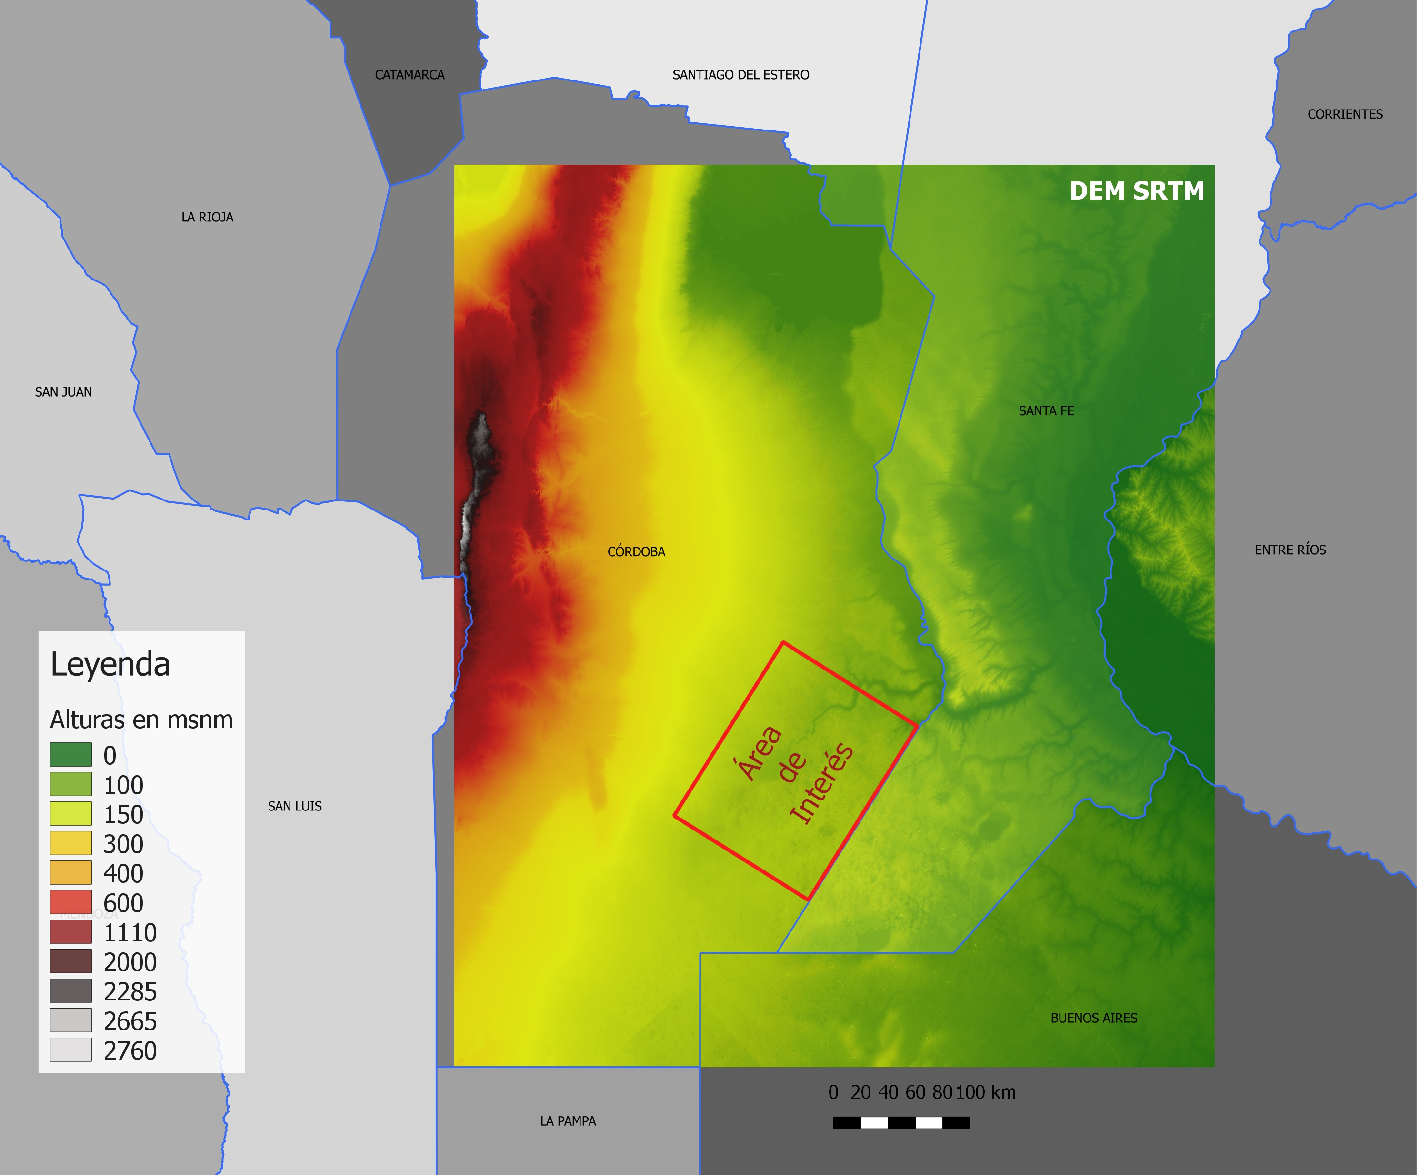
\includegraphics[width=0.85\textwidth]{imagenes/SRTMOriginalAndShape4.pdf}
 \caption{El archivo vectorial del área de interés es un rectángulo, tiene cierto grado de inclinación y está contenido completamente dentro del DEM SRTM}
 \label{SRTMAndShape}
\end{figure}

Existen una gran cantidad de modelos hidrodinámicos que estudian las inundaciones de llanuras pertenecientes a cuencas hídricas. Estos modelos generalmente tienen centrado su interés en predecir el hidrograma del río en distintos puntos para eventos seleccionados, considerando a la llanura circundante más bien como una zona de alimentación de agua al río. De esta forma la inundación está considerada a través del desborde del río y el proceso que se simula es esencialmente escurrimiento superficial en la llanura y en el canal propio del río. Como ejemplo de estos modelos podemos citar entre otros: Mike-11, ONDA, HEC-RAS y LISFLOOD-FP (Bates \textit{et al.} 2011). Estos modelos tienen distintos grados de sofisticación en lo referente a los esquemas de ecuaciones que resuelven, pero como señalan Bates \textit{et al.} (2011), dado que la topografía tiene un peso determinante en la simulación, el uso de esquemas complejos no aseguran un mayor grado de predicción. En tal sentido, es preferible usar esquemas simples que se ajusten al requerimiento de predicción deseado por el usuario y que integren adecuadamente los datos de entrada. Estas características son reunidas por el modelo LISFLOOD-FP, el cual ha sido tomado como base para nuestro modelado.

La zona de estudio, tal como se mencionó, es el sur de la provincia de Córdoba limitante con la provincia de Santa Fe, Carignano \textit{et al.} (2014) describen detalladamente el área de estudio desde una visión geomorfológica la cual contiene los siguientes ambientes:

\textbf{Planicie sudoriental con campos de dunas:} El paisaje de la subunidad está dominado por las megadunas parabólicas y longitudinales, cubriendo en forma discontinua una superficie general sumamente horizontal. Éstas alternan con depresiones  pertenecientes a una paleored fluvial muy probablemente desarrollada por el río Popopis. Actualmente dichas depresiones están transformadas en cañadas y lagunas encadenadas con orientación SO-NE. Un segmento preservado de una de las fajas fluviales aparece al noreste de Arias; tiene 11 km de longitud y de 2 a 3,5 km de ancho y está limitado por un campo de dunas disipado, con diferencias altimétricas máximas de 4 m. Respecto al origen de la cañadas del área, Ferpozzi (1988) interpreta que se trata de bajos o depresiones longitudinales heredadas de paleorrelieves eólicos y que en las condiciones morfogenéticas actuales funcionan concentrando el escurrimiento. Iriondo \textit{et al.} (2007), en cambio, deducen un primer origen fluvial para las mencionadas cañadas.
En el resto del área, los interfluvios en general corresponden a extensas áreas planas y prácticamente horizontales o con pendientes poco perceptibles debido a la disipación casi total de las megadunas. Su superficie fue cementada por procesos pedogénicos y epigenéticos (calcreta), dificultando la infiltración del agua de lluvia y favoreciendo la formación de bañados. Dicha superficie se detectó por debajo de las megadunas parabólicas a una profundidad entre 5,5 y 8 m en el área de Canals a partir de datos de resistividad eléctrica (Iriondo \textit{et al.} 2008). Esta superficie poligénica aparece en superficie o muy cerca de ella (cubierta por dunas disipadas o un manto policíclico de arena eólica) en el área ubicada inmediatamente al sur de La Cesira y al este de Laboulaye (sector Leguizamón-Rosales), extendiéndose en el área ocupada por la laguna La Picasa, en el sudoeste de Santa Fe. Las depresiones tienen forma generalmente circular o elíptica con clara orientación SO-NE. Bajo el clima actual se encuentran en general anegadas y afectadas por procesos limnológicos. Algunas hoyas presentan lunetas a sotavento de la depresión. Un área típica del borde del Mar de Arena Pampeano en la provincia aparece entre las localidades de Cavanagh y Arias. En una distancia de 18 km, el extremo sur de esa transecta está caracterizado por megadunas sobre las que se diferencian pequeñas lomas de 2 a 4 m de altura y depresiones en un patrón irregular, el extremo norte está expresado por un plano dominante, con lomas arenosas y depresiones aisladas (Iriondo \textit{et al.} 2011).

Desde el punto de vista hidrológico, la escasa pendiente hace que no existan canales importantes que permitan conducir el escurrimiento superficial sino que éste se realiza en manto sobre grandes áreas y en escalas de tiempo relativamente largas. En el balance hidrológico general predominan los procesos verticales (evapotranspiración e infiltración) por sobre el escurrimiento. Sin embargo, el escurrimiento superficial es importante para determinar la zona anegada que estará sujeta a los flujos verticales de pérdida. Por otra parte, cada laguna funciona como un reservorio limitado de una microcuenca, pero al superarse su capacidad de almacenamiento se produce escurrimiento superficial encadenando unas con otras y generando un área anegada que las contiene (Masuelli \textit{et al.} 2009).

Dadas las características de la zona estudiada, el modelado tiene en cuenta varios detalles. El hecho de que el terreno sea tan extremadamente plano hace que el DEM que se usa deba estar muy pulido, reduciendo el nivel de ruido de los metros a los centímetros para que el agua no encuentre obstáculo espurios para drenar (Masuelli \textit{et al.} 2009). El no poseer canales importantes hace que el escurrimiento sobre la planicie y la existencia de pequeños bajos conduzca a que éstos se conviertan en zonas anegadas, cuando en los otros modelos este proceso era funcional para obtener la carga del río, el que con su desborde determina dichas zonas. La importancia de los procesos verticales hace que se los deba incluir en el modelo, con la complicación de que estos procesos tienen escalas espaciales y temporales muy distintas.


%***********************************************************************************************




\section{Relevamiento de DEMs para usos hidrológicos}


Entre los sistemas satelitales que ofrecen datos topográficos, se encuentran plataformas cuya información está disponible de manera gratuita, de fácil acceso y con una disponibilidad a nivel global. Entre estos, está el sistema radar SRTM, y el sistema ASTER GDEM (Advanced Spaceborne Thermal Emission and Reflection Radiometer, Global Digital Elevation Model), que se destacan por su alta resolución espacial y disponibilidad global. Si bien, ambos sistemas presentan rangos de precisiones conocidas, son muchos los autores que señalan que ésta dependerá finalmente de las condiciones locales presentes en el área de estudio (Kiamehr \textit{et al.} 2005; Schumann \textit{et al.} 2008; Li \textit{et al.} 2009).

\subsection{Misión SRTM}

Los datos SRTM fueron obtenidos a partir de imágenes de radar tomadas a bordo del Transbordador Espacial Endeavour durante una misión de 11 días de duración que se realizó en Febrero de 2000. El proyecto SRTM es un esfuerzo colaborativo entre la National Aeronautics Space Administration (NASA), la agencia de Inteligencia Geoespacial y el departamento de defensa de los Estados Unidos (NGA), el Centro Aeroespacial Alemán (DLR) y la Agencia Espacial Italiana (ASI). 

El Laboratorio de Propulsión a Reacción de la NASA (Jet Propulsion Laboratory JPL) coordinó la misión y el centro de datos del Servicio Geológico de los Estados Unidos (United States Geological Survey USGS) EROS tiene la responsabilidad de almacenar, distribuir y archivar los productos SRTM finales.

La misión de radar topográfico de NASA a bordo del Shuttle ha provisto datos de elevación digital (DEMs) para un poco más que el 80\% del globo terráqueo. El objetivo fue tomar cada segmento de la tierra al menos dos veces desde diferentes ángulos, uno con pasada ascendente, y otro con pasada descendente, para poder capturar áreas con sombras, debido a la ingeniería del radar. Una descripción más detallada se da en la sección \ref{SRTMeHydroSHEDS}.


\subsection{ASTER GDEM}

La primera versión del ASTER Global Digital Elevation Map (GDEM), publicado en junio de 2009, se ha generado utilizando pares de imágenes estéreo recogidas por el instrumento ASTER a bordo del satélite Terra. La cobertura de ASTER GDEM se extiende desde los 83 grados de latitud norte hasta 83 grados de latitud sur, que abarca el 99 por ciento de la superficie terrestre de la Tierra.

GDEM V2 es una versión mejorada de la primera versión, añade 260.000 pares estéreo adicionales, mejorando la cobertura y reduciendo la ocurrencia de artefactos. El algoritmo de producción refinada proporciona una mejor resolución espacial, una mayor precisión horizontal y vertical, y una mejor cobertura y detección de cuerpos de agua. El ASTER GDEM V2 mantiene el formato GeoTIFF y la misma estructura de grilla y mosaico que la versión V1, con resolución de 1 x 1 grado (lo que equivale a 30 x 30 metros en el ecuador).

La versión 2 muestra mejoras significativas respecto a la versión anterior (como por ejemplo reducción de ruido y resolución vertical). Sin embargo, se aconseja a los usuarios que los datos contienen anomalías y artefactos que impedirán la eficacia para su uso en ciertas aplicaciones (Tachikawa \textit{et al.} 2011).

\subsection{Comparación con SRTM}

Moreno de las Heras \textit{et al.} (2012) realizó un estudio comparando SRTM V4 con ASTER GDEM1 para la determinación de descriptores hidrogeológicos y geomorfológicos y concluyó que SRTM V4 es más confiable que ASTER GDEM1, particularmente en áreas donde ASTER GDEM1 muestra artefactos de elevación (no correspondientes a la superficie terrestre).

Muchos de estos estudios fueron orientados específicamente al uso hidrológico, obteniendo buenos resultados de SRTM en comparación con ASTER GDEM (Forkuor \textit{et al.} 2012).

Algunos estudios usando análisis de área inundada demostraron que GDEM2 tiene mejor calidad que GDEM1 y similar a SRTM y a Topo-DEM, además la precisión vertical de GDEM2 es mucho menor que la de GDEM1, debido a efectos de ondulación (Tachikawa \textit{et al.} 2011).

Otros estudios demostraron que se observa que el DEM SRTM presenta mejores resultados de ajuste con los datos de terreno que ASTER, tanto en términos globales como en cada una de las tipologías de superficie. Por otra parte ambas plataformas presentaron efectos de subestimación o sobreestimación con respecto a puntos de control, los que también estuvieron diferenciados según la tipología de la superficie, siendo positivos (sobrestimación) en zonas de llanura y negativos (subestimación) en cordones. En todos los casos fueron más preponderantes en el sensor ASTER, excepto para las zonas de pradera en llanura (Rozas Vasquez D \textit{et al.} 2009).

El reciente acceso a datos de la banda X del SRTM, con mejor resolución que la banda C, propicia el análisis y validación del mismo. En este caso Díaz \textit{et al.} (2010) evalúan los SRTM C/X y Aster GDEM y su relación con errores planialtimétricos respecto a datos pancromáticos ortorectificados Quickbird (es el satélite comercial con mayor resolución de los disponibles hasta la fecha, ofreciendo imágenes con un tamaño de píxel a partir de 60 cm), concluyendo que el SRTM /X es el más exacto en la zona analizada (El Bolsón, Río Negro). 

En otro trabajo de Burgos (2012) se presentaron comparaciones, ajuste altimétrico y validación de cinco DEM: SRTM en sus versiones v2.1, SRTM30 y SRTM-v4.1 en banda C; SRTM en banda X y ASTER-GDEM. Estos dos últimos con 30 m de resolución y de 90 m los primeros. El objetivo del estudio, es cuantificar el error vertical de cada DEM, y
establecer cuál es el más apropiado, para la aplicación de un modelo hidrodinámico del tramo inferior del río Tunuyán en la provincia de Mendoza y se concluye que SRTM-v4.1 presenta el mayor grado de precisión. 

\section{SRTM e HydroSHEDS}
\label{SRTMeHydroSHEDS}

Los datos de elevación digital SRTM, producidos por NASA originalmente, son un gran avance en la cartografía digital del mundo, y proporcionan un importante avance en la accesibilidad a los datos de elevación de alta calidad para una gran parte de las regiones tropicales y otras zonas del mundo en desarrollo.

A continuación se describe la especificación de las diferentes versiones del DEM SRTM, su evolución y la serie de procesamientos realizados hasta la obtención de HydroSHEDS: un DEM adecuado hidrológicamente.



\subsection{Formato y Disponibilidad}

Este dato es actualmente distribuido libremente por el Servicio Geológico de los Estados Unidos (USGS) y está disponible para ser descargado desde el sitio EarthExplorer del USGS en la sección Digital Elevation-SRTM (https://earthexplorer.usgs.gov/). El SRTM está disponible como dato DEM de 3 arco segundos de resolución (aproximadamente 90m) en el Ecuador, y son provistos en mosaicos de 5 x 5 grados. Todos son producidos a partir de un conjunto de datos continuos para permitir un fácil mosaiqueado. Están disponibles tanto en formato ArcInfo ASCII como en GeoTiff para facilitar su uso en una variedad de procesamiento de imágenes y aplicaciones GIS. Farr \textit{et al.} (2007) proveen una descripción detallada de la misión SRTM.

Las franjas SRTM se extienden desde los 30 grados con respecto al nadir hasta los 58 grados a una altitud de 233 kilómetros, comprendiendo un ancho de 225 kilómetros. Durante el vuelo, el instrumento estuvo activo en todo momento y se tomaron alrededor de 1000 franjas individuales, dentro de los 10 de duración de la misión. El largo de las franjas adquiridas iban desde unos pocos cientos hasta varios miles de kilómetros.

Todos los valores de elevación son enteros binarios con representación de signo y magnitud, correctamente justificados, de 2 bytes. El bit de signo es el más significativo. Valores negativos no son complementados.

Estos valores permiten un rango entre ± 32767 metros, sin embargo en la práctica, la elevación del terreno no deben exceder los +9000 metros o los -12000 metros. Valores nulos son representados por datos con todos los bits seteados en 1, es decir -32767.
Aunque Jarvis \textit{et al.} (2008) hicieron desarrollos para corregir los valores sin datos, aun existen estos píxeles erróneos dentro de la imagen.

Los datos se encuentran en proyección geográfica (Lat/Long), con datum horizontal WGS84 y datum vertical EGM96.

\subsection{Evolución y versiones de SRTM}

Este dato es el resultado de una serie de procesamientos para corrección de agujeros en la imagen. Se siguió el método descripto por Reuter \textit{et al.} (2007). La primera etapa de procesamiento incluye la importación y la fusión de imágenes de un grado de largo en superficies continuas en formato ArcGRID. El segundo proceso se llena agujeros pequeños de forma iterativa y limpia la superficie para reducir huecos y picos. La tercera etapa interpola a través de los huecos utilizando una variedad de métodos. El método utilizado se basa en el tamaño del hueco, y en la forma del relieve que la rodea.

\subsubsection{Datos de elevación SRTM - Versión 1 (Datos sin terminar SRTM-1 y SRTM-3)}

Los datos SRTM crudos han sido procesados por el JPL. Como resultado se obtuvo un conjunto de datos que puede contener numerosos huecos y otros puntos espúreos como anomalías en valores demasiado altos (picos) o demasiado bajos (pozos). Debido a que las superficies de agua producen muy baja retrodispersión del radar, los cuerpos de agua generalmente no están bien definidos y aparecen con bastante ruido, así como las lineas de la costa. Se encuentran disponibles datos con resolución de 1 arcosegundo (SRTM-1) con tamaño de celda aproximado de 30 metros en el ecuador y con resolución de 3 arcosegundos (SRTM-3) con resolución aproximada de 90 metros en el ecuador. Para más detalles ver NASA/JPL (2005).


\subsubsection{Datos de elevación SRTM - Versión 2 (Datos terminados DTED-1 y DTED-3)}
\label{SRTMDefincion}


Después de que JPL completó el procesamiento crudo de SRTM-1 y SRTM-3, NGA realizó verificaciones para asegurar la calidad y luego llevó a cabo varios pasos adicionales para cumplir con los datos estándares requeridos del formato de los Datos Digitales de Elevación de Terreno (Digital Terrain Elevation Data (DTED®)) (NASA 2003). Picos y pozos en los datos fueron detectados y anulados. Pequeñas porciones de valores nulos fueron completados por interpolación de píxeles vecinos. Grandes extensiones de valores nulos, en cambio, conservaron tales valores. El océano fue asignado con una elevación de cero metros. Lagos de 600 metros o más de extensión fueron planchados se les asignó un valor de altura constante. Ríos de más de 183 metros de ancho fueron delineados y decreciendo monótonamente en altura. Las islas fueron tenidas en cuenta si el eje principal superaba los 300 metros o si el relieve era superior a 15 metros. Todas las etapas de acabado se llevaron a cabo en la resolución original de 1 arcosegundo. Más detalles en NASA/JPL (2005).

\subsubsection{Red fluvial vectorizado mundial ArcWorld}
\label{ArcWorldLabel}

El conjunto de datos ArcWorld (ESRI 1992) incluye un mapa vectorial mundial de las masas de agua superficial a una resolución de 1:3 millones. Como parte de su esquema de clasificación, distingue ríos lineales en naturales (permanentes e intermitentes) o artificiales (canales) y proporciona aproximadamente 7000 polígonos de cuerpos de agua abiertos grandes (incluyendo ríos y lagos). Aunque digitalizado a una escala más general, ArcWorld parece incluir algunas correcciones y actualizaciones en comparación con DCW (Digital Chart of the World) y proporciona un enfoque coherente sobre los principales ríos y lagos del mundo.

\subsubsection{Base de datos global de humedales y lagos (Global Lakes and Wetlands Database - GLWD)}
\label{GLWDLabel}
La Base de Datos Global de Lagos y Humedales (Lehner y Döll 2004) combina una diversidad de mapas de humedales y lagos existentes a nivel global (a escala 1:1 a 1:3 millones de resolución) en una cobertura consistente. Provee polígonos de costa de aproximadamente 250.000 lagos y embalses en todo el mundo, incluyendo sus áreas de superficie y otros atributos. En cuanto a los lagos y embalses, GLWD se basa en gran medida en DCW y ArcWorld sino que también incluye varias actualizaciones y correcciones de datos.

\subsubsection{Mapa Digital del Mundo (DCW) red global vectorizada de ríos.}
\label{DCWLabel}

La Carta Digital del Mundo (ESRI 1993) es un mapa vectorial mundial con una resolución de 1:1 millón que incluye una capa de accidentes hidrográficos como ríos y lagos. DCW (también conocido como VMAP-0) es considerado generalmente para proveer los datos de la red mundial de ríos más completos y consistentes disponibles en la actualidad. Se basa en el DMA de Estados Unidos (ahora NGA) Operational Navigation Charts (ONC) cuya información data de la década del 70 a los 90's (Birkett y Mason 1995). La precisión de la posición de DCW varía considerablemente entre las regiones, y no hay distinción entre los ríos naturales y canales artificiales.

\section{Adecuación Hidrológica}


\subsection{HydroSHEDS}
\label{HydroSHEDSDef}

HydroSHEDS (\underline{\textbf{Hydro}}logical data and maps based on \underline{\textbf{SH}}uttle \underline{\textbf{E}}levation \underline{\textbf{D}}erivatives at multiple \underline{\textbf{S}}cales) proporciona información hidrográfica en un formato coherente y global para aplicaciones a escala regional y global. HydroSHEDS ofrece una serie de conjuntos de datos georreferenciados (vector y raster), incluidas las redes de transmisión, los límites de las cuencas hidrográficas, las direcciones de drenaje, y las capas de datos auxiliares tales como acumulaciones de flujo, las distancias y la información de topología del río.

HydroSHEDS se obtiene a partir de los datos de elevación de la Shuttle Radar Topography Mission (SRTM) con una resolución de 3 arcosegundos en el ecuador. Los datos SRTM originales han sido hidrológicamente acondicionados utilizando una secuencia de procedimientos automatizados. Se han aplicado los métodos existentes de mejora de datos y algoritmos desarrollados recientemente, incluyendo el llenado de huecos, el filtrado y las técnicas de ampliación de la escala. Se hicieron correcciones manuales cuando fue necesario. Las evaluaciones preliminares indican que la calidad de la exactitud de HydroSHEDS supera con creces la de los mapas de cuencas hidrográficas y mundiales existentes.

El objetivo de desarrollar HydroSHEDS fue generar capas de datos clave para respaldar los análisis regionales y globales de las cuencas hidrográficas, la modelización hidrológica y planificación de la conservación de agua dulce con una calidad, resolución y alcance que anteriormente no se podían alcanzar. Las resoluciones disponibles varían desde 3 segundos de arco (aprox. 90 metros en el ecuador) hasta 5 minutos (aprox 10 Km. en el ecuador) con una extensión casi global sin igual (Lehner \textit{et al.} 2006).

El objetivo del desarrollo de HydroSHEDS fue generar capas de datos clave para respaldar los análisis de cuencas hidrográficas regionales y mundiales, y la planificación de la conservación de agua dulce con una calidad, resolución y alcance que anteriormente no se podían alcanzar. Las resoluciones disponibles varían desde 3 segundos de arco (aproximadamente 90 metros en el ecuador) hasta 5 minutos (aproximadamente 10 km en el ecuador) con una extensión casi global sin igual.


HydroSHEDS ha sido desarrollado por el Programa de Ciencia de la Conservación del Fondo Mundial para la Naturaleza (WWF - World Wildlife Fund), en colaboración con el US Geological Survey (USGS), el Centro Internacional de Agricultura Tropical (CIAT), The Nature Conservancy (TNC), y el Centro para el Medio Ambiente sistemas de Investigación (CESR) de la Universidad de Kassel, Alemania. Los fondos principales para este proyecto fueron proporcionado a WWF por Johnson Diversey, Inc.

\subsubsection{Correcciones}


%\subsubsubsection{Corrección de huecos}

Como primer procesamiento de HydroSHEDS se realizó una serie de pasos para obtener un modelo de elevación para el cual se hayan corregido datos faltantes o llenado de huecos. 

Los datos iniciales de base para el resultado final son los productos SRTM-3 y DTED-1. A partir de estos productos se realizó una combinación de ambos para el inicio del procesos de corrección de huecos.

\textbf{Combinación de SRTM-3 sin terminar y datos DTED-1 terminados.}

Después de realizar una serie de pruebas locales, se decidió aplicar una combinación de datos SRTM-3 y DTED-1. Para cada píxel se usó el valor mínimo de cualquiera de los DEM, ya sea en SRTM-3 o en DTED-1 para generar un modelo de elevación inicial HydroSHEDS elevación. El requerimiento mínimo conserva la menor de las dos superficies en los datos de elevación combinados, los cuales se consideran deseable para la identificación posterior de direcciones de drenaje.

Luego se fueron aplicando distintos algoritmos secuencialmente, con la finalidad de obtener un producto de mejor calidad en donde no existan huecos. Entre estos algoritmos se encuentran:

\begin{itemize}
	\item Identificación de Líneas costeras de mares y océanos
	\item Cambio en resolución de datos: Para evitar solapamientos en bordes del mosaiqueado.
	\item Algoritmo CIAT
	\item Algoritmo HydroSHEDS
	\item Combinación de los algoritmo mencionados
\end{itemize}

%Se obtiene como resultado el producto HydroSHEDS DEM con resolución de 3 segundos (90 mts).

\textbf{Identificación de depresiones}

Típicamente un DEM presenta una gran cantidad de piletas o depresiones. Estos son conjuntos de píxeles completamente rodeados por otros con mayores valores de altura. En muchos casos estas piletas o depresiones son consideradas espúreas. Estas depresiones espurias son problemas críticos en aplicaciones hidrológicas ya que interrumpen el flujo continuo a través de la superficie DEM. Es por eso que, son típicamente removidas del DEM antes derivar una red fluvial.

La decisión de depresiones naturales o espúreas fue determinada a partir de un análisis en GIS hecho de forma manual. Las depresiones con más de 10 metros de profundidad y más de 10 kilómetros cuadrados de superficie fueron destacadas como potenciales piletas naturales. Luego fueron revisadas visualmente y comparadas con información del DCW, ArcWorld, GLWD para determinar su validez como piletas. El proceso de identificación de piletas manual es subjetiva, y en muchos casos la definición de las depresiones naturales es difícil y ambigua.


\subsubsection{Procesos de adecuación hidrológica aplicados a HydroSHEDS}

Además de los sumideros, los DEM originales muestran una serie de otras características, objetos y anomalías que pueden causar problemas o errores significativos en aplicaciones hidrológicas.

La característica más significativa es probablemente el hecho de que los valores de elevación de SRTM, siendo un producto derivado de radar, se ven influidos por la cubierta vegetal. En las zonas de bajo relieve, estas pequeñas desviaciones de la verdadera altura de la superficie pueden causar errores significativos en la definición de cursos de los ríos y direcciones de flujo.


Con el fin de mejorar el rendimiento de un DEM para aplicaciones hidrológicas, existe una serie de procesos y procedimientos GIS que se aplican de forma procedimental. Sin embargo, debido a las características individuales de los diferentes DEM y, a escala global, debido a las variaciones regionales en el tipo de errores, no existe un método que aborde todos los problemas posibles. Para HydroSHEDS, una secuencia de procedimientos de acondicionamiento hidrológico fueron implementado, ya sea una adaptación de la funcionalidad estándar de GIS, nuevo desarrollo, o personalizado. El enfoque general fue llegar a un compromiso entre: forzar al DEM para producir correcta topología de red fluvial, particularmente para los ríos más largos, preservando al mismo tiempo la mayor información SRTM original como sea posible. Notar que en cualquier caso el proceso de acondicionamiento altera los datos de elevación originales y puede inutilizarlos para otras aplicaciones.

Uno de los productos intermedios de SRTM es SWBD (SRTM Water Body Data) en el cual fueron identificados oceanos, lagos y ríos.

Los siguientes procedimientos de acondicionamiento hidrológicos se han aplicado a los datos de elevación HydroSHEDS:


\begin{itemize}
	\item \textbf{Profundización de la superficie de aguas abiertas:} Todos los ríos y lagos, identificados en SWBD fueron cavados en 10 metros con el fin de forzar el flujo derivado de mantenerse dentro de estos objetos. Así como los vacíos sin datos en los datos de elevación SRTM originales pueden indicar superficies de agua, todas las áreas de no datos y vacío se redujeron en 10 metros también. El umbral de 10 metros fue elegido como el que representa un efecto suficientemente fuerte en áreas planas (donde la identificación de los cauces de los ríos y lagos es particularmente difícil), mientras que produce solo insignificantes cambios en áreas con pendientes más pronunciadas (donde la existencia de no datos son probablemente causados por la sombra de radar en lugar de aguas abiertas).
	
	\item \textbf{El deshierbe de las zonas costeras:} En el modelo de elevación obtenido por radar, los manglares o cinturones de vegetación costeros pueden ser interpretados como un bajo pero continuo terraplén que bloquea cualquier flujo directo hacia el océano. En el modelo de la red fluvial obtenida, estas barreras pueden provocar significativos efectos de remansos. Para reducir este efecto, la zona costera, es decir, un buffer de ancho 0,02 grados (aproximadamente 2 km en el ecuador) a lo largo de la costa del océano fueron desmalezados mediante la reducción de 5 metros cada tres celulas al azar. Este cambio sutil, en combinación con los siguientes filtros, obliga ocasionales rupturas o pasos de agua en los diques costeros ligeramente elevados.
	
	\item \textbf{Demarcación de flujos de agua:} El más importante proceso de adecuación en la generación de HydroSHEDS ha sido el llamado procedimiento de "Stream Burning", que es la demarcación de flujos de agua. La demarcación de flujos de agua es un proceso que se utiliza a menudo para establecer el curso de los ríos conocidos en la superficie. Los valores de altura a lo largo de los ríos, como se describió por ejemplo, en una capa vectorial existente, son reducidos a un cierto valor, por lo que demarca gargantas profundas en la elevación de la superficie. La demarcación puede ser extendida para incluir un buffer alrededor de las líneas de los ríos con el fin de dar moldear una transición más suave entre la superficie original y la garganta. Para HydroSHEDS, sólo los grandes ríos y lagos fueron demarcados en la superficie de elevación con el fin de evitar alteraciones excesivas de la superficie SRTM. Se utilizaron todos los ríos permanentes e intermitentes y lagos de ArcWorld (Sección \ref{ArcWorldLabel}), así como todos los ríos y lagos de GLWD (Sección \ref{GLWDLabel}), mientras que los de resolución mayor pero no clasificados de DCW se omitieron. Dado que la exactitud de los mapas globales existentes es desconocida, se hicieron ensayos para minimizar el impacto de estos conjuntos de datos en los datos de SRTM. Después de múltiples pruebas, la profundidad de la demarcación de los ríos se fijó a 12 metros, con un buffer de 0.005 grados (aproximadamente 500 metros en el ecuador) alrededor de los cursos de ríos. La profundidad de demarcación se redujo, de manera escalonada, de 12 metros en la hondonada a 2 metros en el borde de la linea de separación. Lagos fueron demarcados con una profundidad de 14 metros y una distancia de separación de 0,0025 grados. El ajuste de parámetros se orientó a notable refuerzo de los principales ríos de zonas planas, donde de otro modo la correcta delimitación de los ríos es difícil. En las regiones escarpadas, las pequeñas profundidades demarcadas resultan más bien en cambios insignificantes de la superficie de elevación, por lo tanto, los datos de SRTM mantienen la información dominante para derivar direcciones de drenaje.	
	
	\item \textbf{Filtrado:} A continuación, se filtró toda la superficie elevada aplicando un análisis de vecinos direccional de 3x3. Los valores de elevación de todas las posibles trayectorias de flujo ángulo rectos y obtusos en una ventana de 3x3 fueron promediados y se les asignó el valor mínimo a la celda central. Este filtro tiene como objetivo eliminar los restantes picos y pozos, preservando y haciendo cumplir los cursos fluviales lineales y el fondo de los valles. En particular, los píxeles individuales que puedan bloquear una vía de flujo continuo son eliminados.
	\item \textbf{Moldeo de cursos valle} Luego, los valles fueron expuestos a través de un análisis del terreno de píxeles cercanos, y fueron profundizados en 3 metros. Los valles fueron identificados por medio de un filtro de mediana de 5x5 combinado con un algoritmo de afinamiento de grilla para detectar características lineales. Este procedimiento de moldeado de valles ha sido desarrollado específicamente para mejorar las delineaciones de los ríos en tierras bajas tropicales removiendo pequeños obstáculos en valles poco profundos. Debido a la pequeña profundización de 3 metros, no se producen cambios significativos en las zonas con relieve más fuerte.
	\item \textbf{Rellenado de piletones}
	En un proceso estándar, todos los piletones espurios en la superficie fueron llenados. Piletones naturales fueron removidos con el fin de excluirlos de la eliminación	
	\item \textbf{Escarbado a través de barreras:} Después de llenar las depresiones, un mapa del río fue generado a partir de los datos de elevación ya procesados. Los principales cursos de ríos, definidos como ríos con un área de cuenca aguas arriba de más de 1000 celdas (aproximadamente 8 km\textsuperscript{2} en el ecuador), fueron plasmados. Los principales ríos, fueron proyectados en el modelo de elevación HydroSHEDS inicial, y todas los ascensos en elevaciones río abajo fueron identificadas. Estos aumentos en la elevación de la superficie original, los cuales obviamente han sido removidos a través de la aplicación de filtros o llenado de depresiones en el proceso de adecuación, pueden representar presas, puentes, muros de contención de cualquier tipo, o gargantas estrechas que bloquean la vía de flujo. En muchos de estos casos, el efecto de llenado de depresiones (es decir, la elevación y el aplanamiento implícito de la zona embalsada) puede no ser deseable la corrección. Para minimizar este efecto, se realizó una segunda iteración del proceso de adecuación: primero, todas las elevaciones crecientes a lo largo de los principales cursos de agua fueron nivelados en los datos iniciales de elevación mediante la reducción adecuada de sus alturas respectivas, luego cavando a través de las barreras. Después de este proceso, todos los demás procesamientos de adecuación fueron repetidos.
	
	\item \textbf{Correcciones Manuales:} La red de ríos derivada fue comparada visualmente con los ríos que se pueden encontrar en otras fuentes de datos con DCW (Sección \ref{DCWLabel}) o ArcWorld (Sección \ref{ArcWorldLabel}). 
	
\end{itemize}


\textbf{Evaluaciones de Calidad de HydroSHEDS}

Lehner \textit{et al.} (2006) también exhiben algunas comparaciones con conjuntos de datos hidrográficos globales y pudieron demostrar que:

\begin{itemize}
	\item En general, HydroSHEDS muestra significativamente mejor precisión que HYDRO1k debido a que HydroSHEDS está basado en un modelo de elevación digital superior.
	\item En general, HydroSHEDS muestra significativamente mejor precisión que ArcWorld (Sección \ref{ArcWorldLabel}) (incluso en áreas con algunas dificultades), es por esto que ArcWorld ha sido incorporado en el proceso de adecuación de HydroSHEDS.
	\item En general, HydroSHEDS muestra significativamente mejor precisión que DCW. Sin embargo, la precisión de ambos conjuntos de datos varía dependiendo de la zona. En algunas regiones en donde HydroSHEDS es susceptible a errores, como en planicies inundables con vegetación, la calidad de DCW puede ser superior.	
\end{itemize}

%***********************************************************************************************




\subsection{Una aplicación a la llanura Bonaerense}
\label{trabajoSergioAntecedente}

Otro antecedente de adecuación del DEM para usos hidrológicos es el trabajo realizado por Masuelli \textit{et al.} (2009). Dicho trabajo fue realizado con el DEM SRTM como base y los procesamiento aplicados fueron realizados de manera manual. Presentaba 3 inconvenientes principales a resolver:

\begin{itemize}
	\item \textbf{Cortinas de árboles:} El DEM del SRTM que se baja por Internet tiene esencialmente la información en un estado crudo por cuanto la altura que muestra para cada píxel tiene que ver con la primera superficie reflectante, es decir por ejemplo que está dando cuenta del tope de la foresta y no del suelo en si mismo (Miliaresis \textit{et al.} 2009). Para nuestra aplicación en hidrología, puede darse la paradoja de que los cursos naturales de drenaje, al poseer generalmente monte en sus inmediaciones, tengan en el DEM una altura mayor que su entorno y por lo tanto, para el DEM no procesado, significar un obstáculo en vez de una vía de escurrimiento.
	\item \textbf{Datos espúreos:} Además es reconocido por el USGS que estos datos tienen algunas fallas, como ser datos extremadamente altos o extremadamente bajos, especialmente en zonas que involucran cuerpos de agua pues su nivel de retrodispersión es muy bajo y así su procesamiento es generalmente muy ruidoso y por lo tanto el DEM obtenido es generalmente muy ruidoso (Lehner \textit{et al.} 2006). Es claro que los datos espurios que tiene pueden determinar la total imposibilidad para un uso específico mientras que para otra aplicación pueden resultar éstos irrelevantes.
	\item \textbf{Bandeado:} Para zonas muy planas está presente un ruido de baja frecuencia de 1 metro de amplitud que es notable en zonas de llanura en dirección NO-SE aproximadamente. El origen de estas franjas se debe a que las imágenes usadas para obtener este DEM son de modo ScanSAR (Masuelli \textit{et al.} 2009). El uso directo de este DEM para modelos hidrológicos en zonas de llanuras puede ser muy problemático. Por cuestiones de estabilidad numérica para pendientes inferiores a 1:100 y para celdas de 100m se necesitan precisiones verticales del orden de algunos centímetros. La metodología planteada es para implementar los siguientes objetivos: Filtrar el ruido de baja amplitud y frecuencia media; filtrar las arboledas y corregir la topografía aledaña a las lagunas.	
\end{itemize}


En dicho trabajo, que fue investigado como antedecente y que se toma como base del presente trabajo, estos problemas fueron resueltas siguiendo la secuencia de pasos expuestos en la figura \ref{metodologiaSergio}:

\begin{figure}[!htb]
   \centering      
   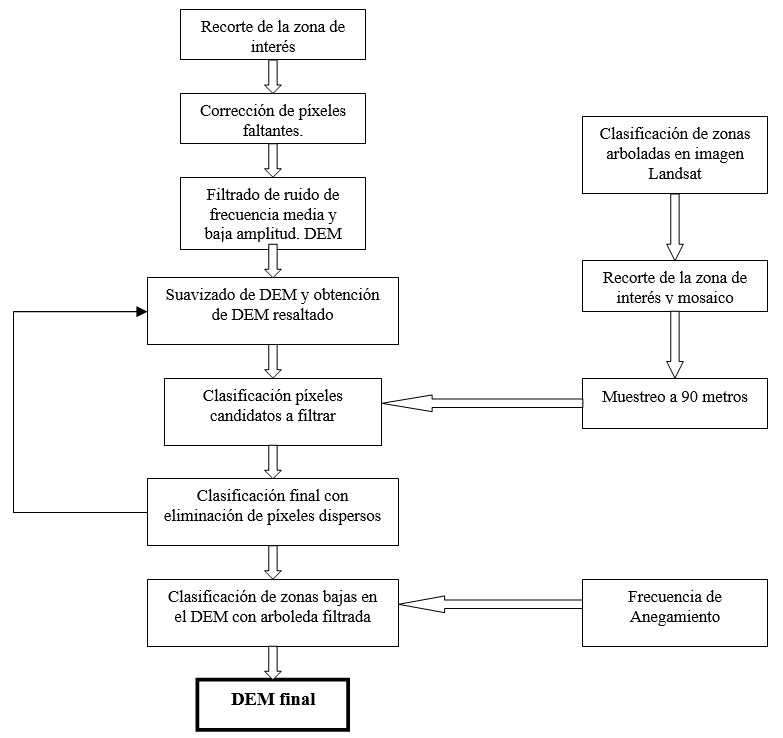
\includegraphics[width=0.85\textwidth]{imagenes/metodologiaSergio.jpg}
 \caption{Diagrama de flujo de los procesos para la obtención del DEM adecuado (Masuelli \textit{et al.} 2009}.
 \label{metodologiaSergio}
\end{figure}

\subsubsection{Corrección de píxeles faltantes}

Los píxeles con datos faltantes en el DEM de entrada se completaron con los valores de los vecinos más próximos.

\subsubsection{Filtrado de ruido de frecuencia media y baja amplitud}

Se midieron sobre la imagen las frecuencias en vertical y en horizontal. Luego, sobre la imagen transformada de Fourier se buscaron las regiones correspondientes a la frecuencia medida y sus armónicas y se las eliminó. Antitransformando se obtiene la imagen filtrada.

\subsubsection{Filtrado de la arboleda}

\begin{itemize}
	\item \textbf{Clasificación de zonas arboladas en imagen Landsat:} Se realizó una clasificación supervisada en imágenes Landsat mediante el método del paralelepípedo de zonas con firmas espectrales similares a bosque.
	\item \textbf{Recorte de la zona de interés y mosaico.}
	\item \textbf{Muestreo a 90 metros:} Luego, esta clasificación fue submuestreada a píxeles de 90 metros de lado. 
	\item \textbf{Énfasis de rasgos sobresalientes en DEM:}	
	\begin{itemize}
		\item \textbf{Filtro cuadrático:} Se obtuvo a partir de la imagen original subdividiendo la imagen original en cuadrados de 10 píxeles de lado, calculando el valor medio sobre cada uno y luego interpolando cuadráticamente en ambas direcciones para cada punto interior del mismo. 
		\item \textbf{Imagen resaltada:} Se obtuvo a partir de la diferencia entre la imagen original y la imagen filtrada cuadráticamente.
	\end{itemize}
	\item \textbf{Clasificación de arboledas:} Para clasificar los píxeles candidatos a corresponder a zonas arboladas se determinó en el DEM resaltado aquellos que correspondieran a árboles en la clasificación del Landsat y con alturas mayores a 4,5m. Luego en forma iterativa se hizo crecer la clasificación a los píxeles contiguos con alturas mayores a 2m. Finalmente, se eliminaron píxeles dispersos.
	\item \textbf{DEM Enfatizado corregido:} Una vez identificadas las arboledas, estos valores son directamente llevados a cero en el DEM enfatizado.	
	\item \textbf{DEM con arboledas corregidas:} El DEM final sin arboledas resulta de la recuperación del DEM por medio de la suma del DEM con filtro cuadrático y el enfatizado sin arboledas detectadas.	
\end{itemize}

\subsubsection{Corrección para zonas bajas}

Se excavó directamente usando la clasificación de frecuencia de anegamiento sobre el DEM a partir de un valor de frecuencia de anegamiento realizada por Vázquez \textit{et al.} (2007) en base a una larga serie histórica de imágenes Landsat del área de estudio (200 imágenes). El criterio elegido fue restar 10cm al DEM por cada 10 \% de esta frecuencia, a partir del valor de 30 \%.


\subsubsection{Filtrado de alta frecuencia}

Luego de las correcciones anteriores, persiste en el DEM el ruido de alta frecuencia que complica su utilización para modelos hidrológicos. Téngase presente que su resolución en altura (no su error) es de un metro y que para la región extremadamente plana en que se está tratando de usar y teniendo en cuenta el espaciamiento entre puntos de grilla de 90 metros de lado, el terreno se presenta muy fragmentado de modo que prácticamente el agua sólo podría fluir, en el mejor de los casos, en trayectos cortos de muy pocos píxeles.

Por lo tanto, para que el agua fluya, la discretización en altura debe ser del orden de algunos cm. Para lograr esto, se le aplicó al DEM un filtro cuadrático de nueve puntos en las direcciones vertical, horizontal y las diagonales principales. El efecto es que suavizan las alturas entre los píxeles vecinos pero respetando las alturas mínimas y máximas locales, lo que en un filtro de media común los valores de los píxeles se verían severamente afectados.


\chapter{Procesamiento del DEM}
\label{chap:procDEM}

En este capítulo se describe el desarrollo de los procesamientos aplicados para obtención de un DEM adecuado hidrológicamente y la metodología para la evaluación de los resultados.


Por lo desarrollado en el capítulo anterior el DEM candidato a usarse en modelado hidrológico sobre el área de interés (Este de la provincia de Córdoba) tendría que ser el HydroSHEDS.

Sin embargo, en la figura \ref{HSHEDSPaleta} pueden observarse claramente 2 defectos importantes: bandeado de baja amplitud y cortinas de árboles. Ambos defectos son corregidos por Masuelli \textit{et al.} (2009), tal como ha sido presentado en la sección \ref{trabajoSergioAntecedente}, y cuyo impacto negativo para realizar simulaciones sobre llanuras ha sido demostrado en dicho trabajo.


\begin{figure}[!htb]
   \centering      
   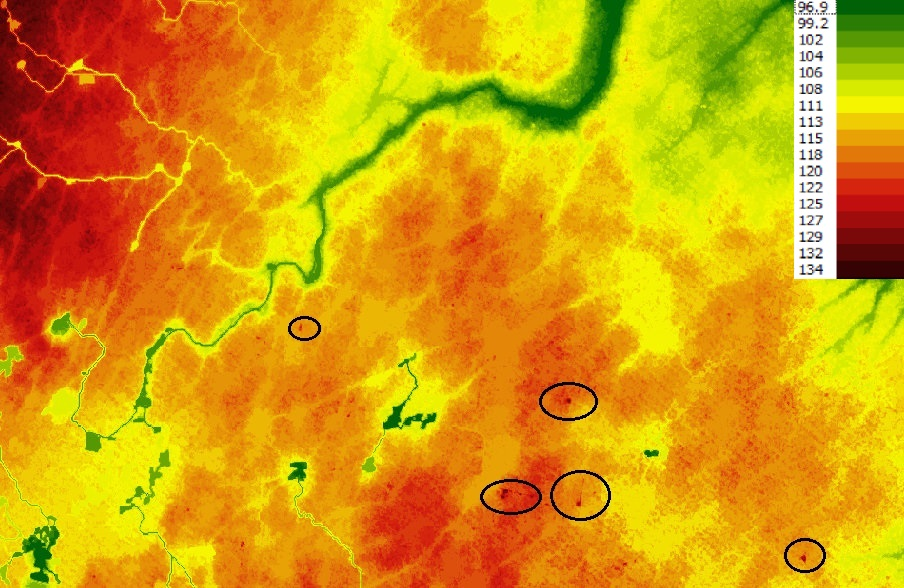
\includegraphics[width=0.85\textwidth]{imagenes/HSHEDSPaleta.jpg}
 \caption{DEM HydroSHEDS en paleta de colores en donde se puede observar el bandeado y las cortinas de árboles localizadas con elipses.}
 \label{HSHEDSPaleta}
\end{figure}


En vista de este problema el presente trabajo consiste en obtener un DEM corregido a partir de la información de SRTM e HydroSHEDS, aplicando las distintas correcciones sobre uno u otro DEM según se considere más conveniente.

\section{Primeras Pruebas}


Inicialmente se abordaron los problemas de bandeado y cortinas de árboles al DEM HydroSHEDS, en cada caso de corrección se encontraron algunos comportamientos no esperados que se describen a continuación:

\subsection{Aplicación de corrección de bandeado a HydroSHEDS}
\label{aplicacionBandeado}

Como vimos en la figura \ref{HSHEDSPaleta} HydroSHEDS presenta el problema de bandedado, por lo que se aplicó la corrección utilizando el método de transformada de Fourier. El resultado no fue satisfactorio como podemos observar en las siguientes figuras:

\begin{figure}[!htb]
   \begin{minipage}{0.48\textwidth}
			\centering
			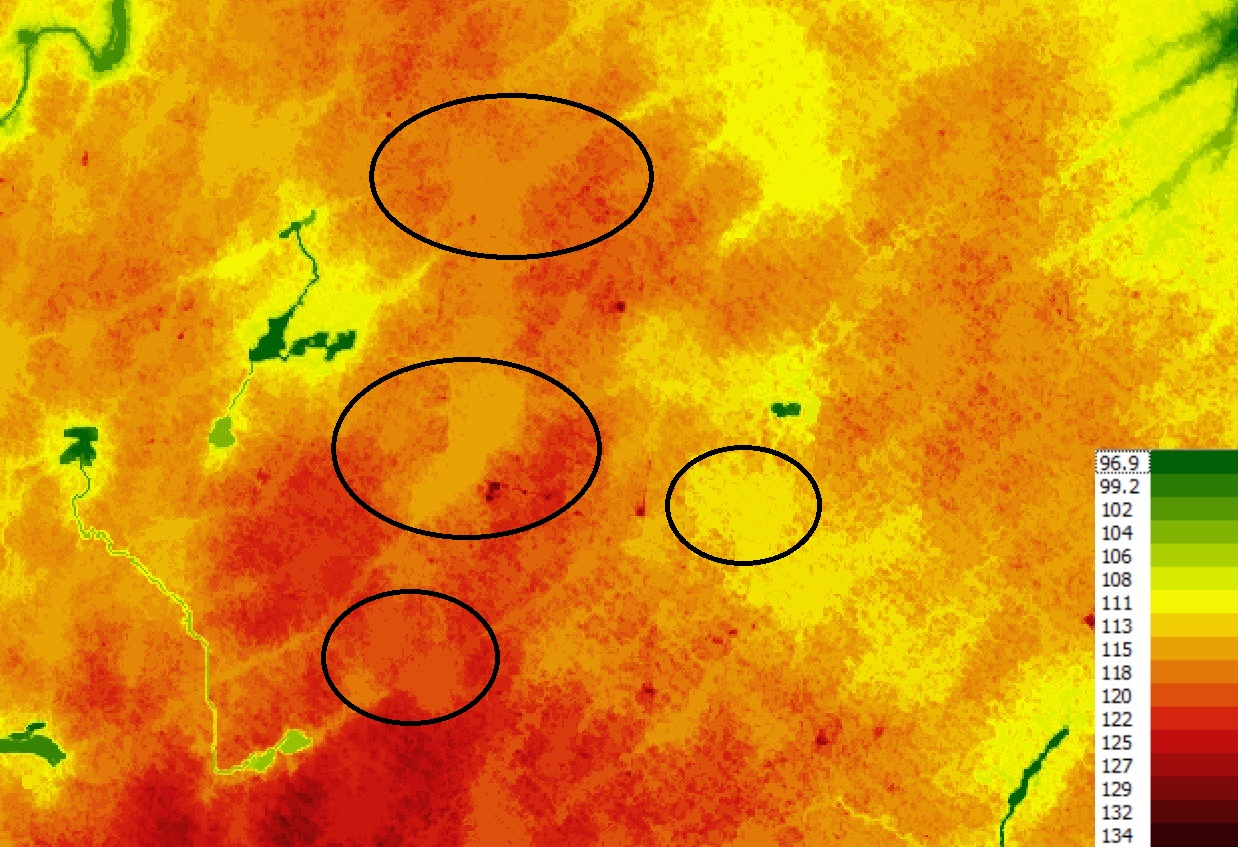
\includegraphics[width=1.0\linewidth]{imagenes/HydroSHEDSBandeadoZoom.jpg}
			\caption{DEM HydroSHEDS con paleta de colores adecuada para resaltar el bandeado en áreas sin lagunas (denotadas con elipses).}
			\label{HydroSHEDSBandeadoZoom}
   \end{minipage}\hfill
   \begin {minipage}{0.48\textwidth}
			\centering
			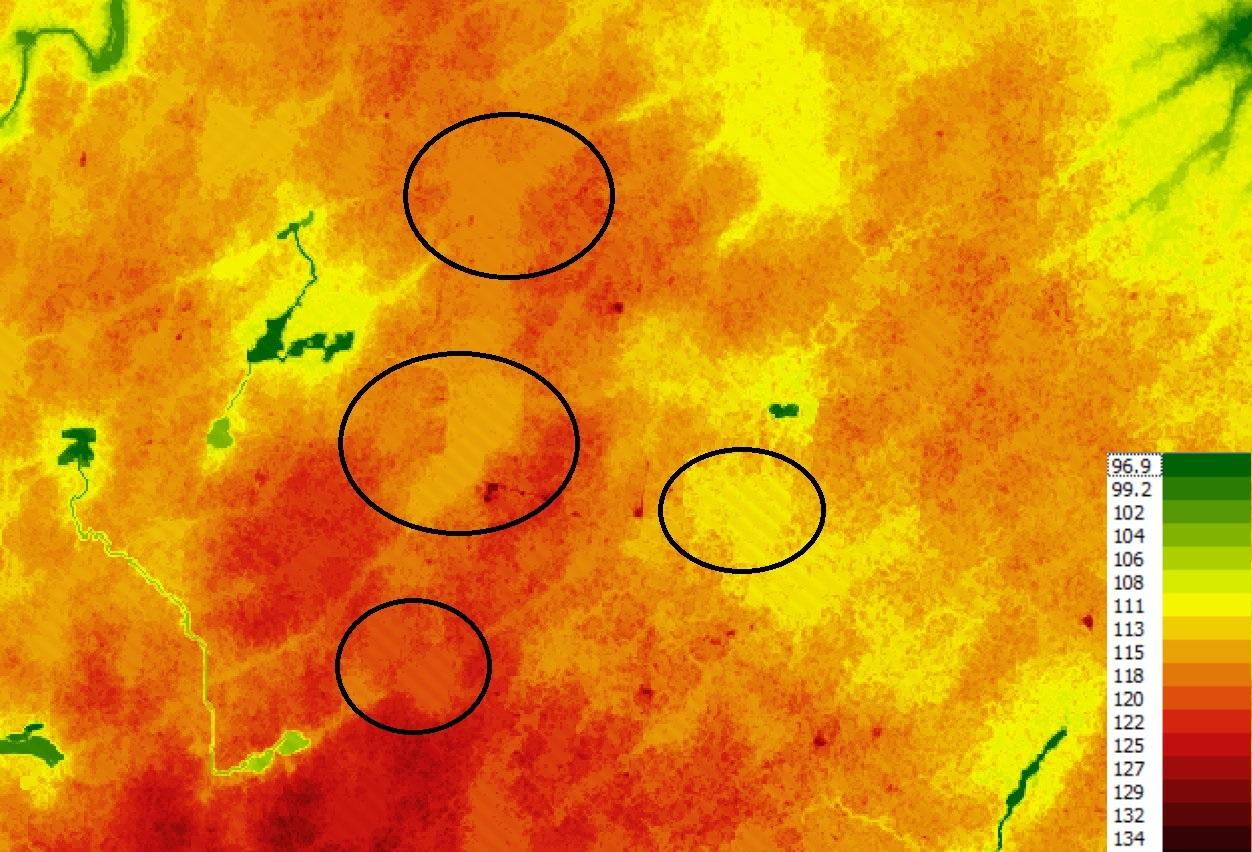
\includegraphics[width=1.0\linewidth]{imagenes/HydroSHEDSBandeadoZoomFourier.jpg}
			\caption{DEM HydroSHEDS en donde podemos distinguir que el bandeado se trasladó del área sin lagunas a las lagunas.}
			\label{HydroSHEDSBandeadoZoomFourier}
   \end{minipage}
\end{figure}

Podemos observar en la figura \ref{HydroSHEDSBandeadoZoom}, un zoom de la figura \ref{HSHEDSPaleta} para distinguir más de cerca el bandeado. A la derecha (figura \ref{HydroSHEDSBandeadoZoomFourier}) observamos la aplicación de la corrección de Fourier en la misma zona que aparece en la figura de la izquierda. Se distingue claramente que el bandeado se trasladó de las áreas sin lagunas a las lagunas. Esto es un efecto no deseado en el uso del DEM de manera hidrológica.



\subsection{Aplicación de corrección de cortinas de árboles a HydroSHEDS}

De igual manera se aplicó la corrección de cortinas de árboles al DEM HydroSHEDS siguiendo el procedimiento de Masuelli \textit{et al.} (2009) proveyendo también resultados no satisfactorios (Figuras \ref{HydroSHEDSTreesZoom} y \ref{HydroSHEDSTreesZoomCorrected}).


\begin{figure}[!htb]
   \begin{minipage}{0.48\textwidth}
			\centering
			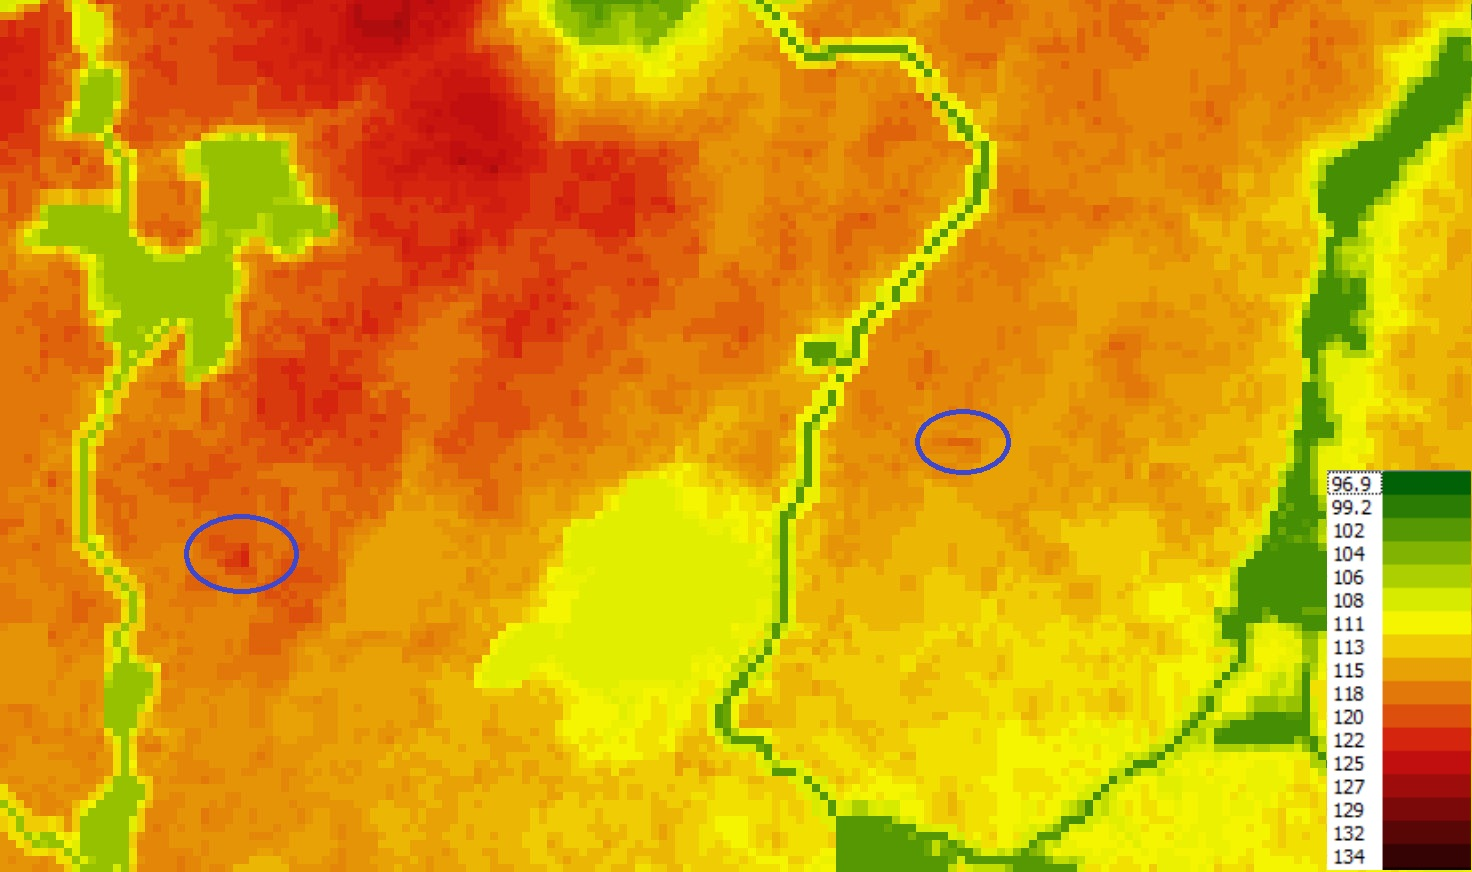
\includegraphics[width=1.0\linewidth]{imagenes/HydroSHEDSTreesZoom.jpg}
			\caption{DEM HydroSHEDS sin haber aplicado la corrección de cortinas de árboles. Observamos destacado en azul la presencia de cortinas de árboles no deseadas y objetivo de la corrección.}
			\label{HydroSHEDSTreesZoom}
   \end{minipage}\hfill
   \begin {minipage}{0.48\textwidth}
			\centering
			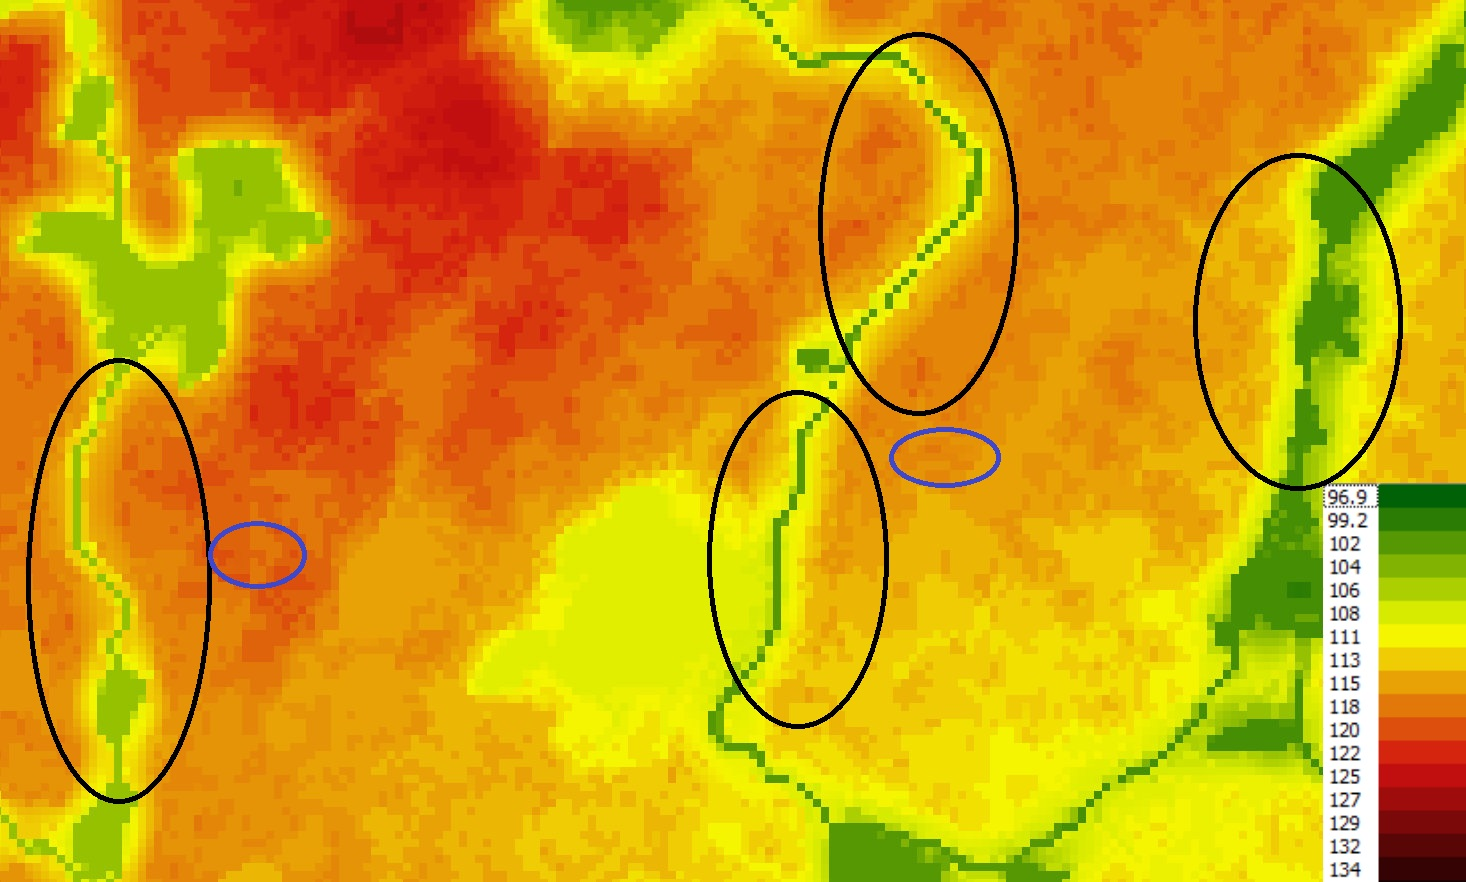
\includegraphics[width=1.0\linewidth]{imagenes/HydroSHEDSTreesZoomCorrected.jpg}
			\caption{DEM HydroSHEDS en donde podemos distinguir los errores no deseados en lo que respecta a los bordes de las cañadas, destacados con elipses negras. Además con azul observamos que las cortinas de árboles fueron corregidas.}
			\label{HydroSHEDSTreesZoomCorrected}
   \end{minipage}
\end{figure}

En este caso, observamos que la aplicación de la corrección a cortinas de árboles resuelve el problema de las cortinas de árboles, pero provee resultados no deseados en lo que respecta a los bordes de cañadas como podemos observar en las zonas destacas en la figura \ref{HydroSHEDSTreesZoomCorrected} en comparación con la figura \ref{HydroSHEDSTreesZoom}. Se puede observar que se generan alturas en los bordes de las cañadas, y esto podría implicar que al momento de usarlo con fines hidrológicos, el agua fuera de la cañada no desemboque en la misma. 



\section{Propuesta a implementar}

Por lo mencionado anteriormente se ve que no es factible el uso de HydroSHEDS aplicando solo las correcciones antes mencionadas. De igual manera es notable las mejoras que provee HydroSHEDS en cuanto a lagunas y cañadas respecto de SRTM. Es por eso que en este trabajo se combina lo mejor de ambos DEM, con los procesamientos necesarios de correcciones y de extracción de información según corresponda.

A partir de esto se toma como metodología la utilizada en el trabajo de preprocesamiento del DEM (Masuelli \textit{et al.} 2009) realizado como parte del antecedente del modelo hidrológico y descripto en la sección \ref{trabajoSergioAntecedente}. Este trabajo explica y describe la secuencia de pasos realizados para llegar a un DEM mejorado para usos hidrológicos a partir de un DEM SRTM. Con el objetivo del uso de modelos hidrológicos en diferentes áreas de estudio, los procesos aplicados en el trabajo de base fueron estudiados, implementados en python y automatizados. Además se agregaron a esta implementación y automatización procesamientos que fueron realizados sobre el DEM HydroSHEDS y luego combinados con los procesos realizados al DEM SRTM.


En resumen se detallan ventajas y desventajas de cada DEM:

\begin{itemize}
	\item \textbf{SRTM:} La corrección del bandeado aplicando Fourier genera resultados satisfactorios. Además aplicar el filtro de suavizado cuadrático no genera problemas en zona de cañadas como si ocurre para HydroSHEDS.
	\item \textbf{HydroSHEDS:} Se supuso que aplicar la corrección del bandeado por el método de Fourier, haría factible el uso de este DEM, pero esta corrección introduce errores en zonas de lagunas o cañadas en donde se aplicaron otros metodos de mejoras. De manera similar, en el proceso de detección de árboles, al aplicar el filtro cuadrático se observaron valores muy altos en zonas de bordes de cañadas. Por otra parte, se considera que HydroSHEDS provee un socavado de cañadas y lagunas muy bien logrado.	
\end{itemize}

Como resultado del análisis de ambos DEM se determinó que proveían diferentes ventajas y una combinación entre ellos proporcionaría mejores resultados. (Tabla: \ref{tablaCombinacion}).

\begin{table}[H]
   \centering      
   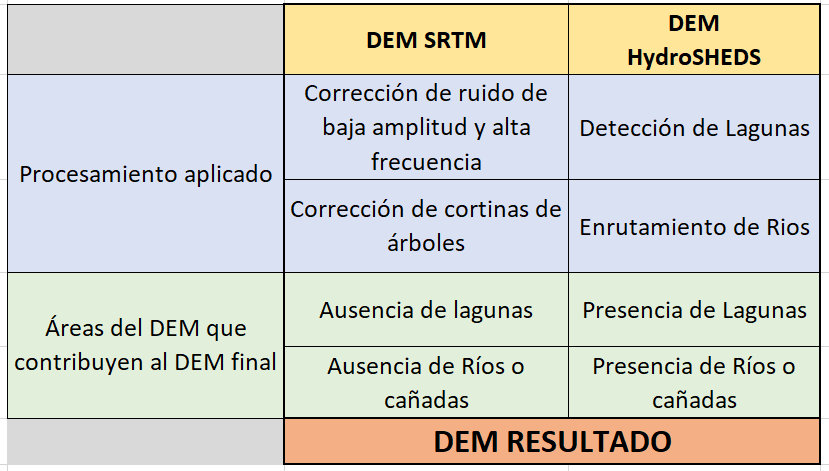
\includegraphics[width=0.6\textwidth]{imagenes/tablaCombinacion.jpg}
 \caption{Procesos aplicados a cada DEM de entrada y contribución al DEM Resultado de este trabajo.}
 \label{tablaCombinacion}
\end{table}

Teniendo como base el trabajo descripto en la sección \ref{trabajoSergioAntecedente}, en este trabajo se desarrollaron procesos para resolver las características mencionadas existentes en el DEM SRTM. A partir de esta base se determinó cuales de estos procesos se implementarían, se refinaron, en algunos casos se mejoraron, se hicieron múltiples pruebas y se automatizó casi en su totalidad el proceso de los DEMs.

El proyecto de software desarrollado puede ser encontrado de manera libre en GitHub, en donde se puede encontrar la documentación adecuada para su correcta ejecución: 

\hyperref[https://github.com/CGuerreroCordova/DEMpreProcPy]{https://github.com/CGuerreroCordova/DEMpreProcPy}

\section{Desarrollo}

\subsection{Automatización del procesamiento:} Además de describir detalladamente los procesamientos aplicados al DEM para la correcta ejecución del simulador hidrológico, se provee la aplicación desarrollada en Python, que permite fácilmente procesar un DEM de llanura para cualquier área de estudio elegida.

Asimismo, para llegar a obtener tal combinación de ambos DEMs se realizó una secuencia de operaciones entre raster las cuales son descriptas a continuación. Este procesamiento respeta el siguiente diagrama de flujo (Figura. \ref{FlowCompleto}):

\begin{figure}[!htb]
   \centering      
   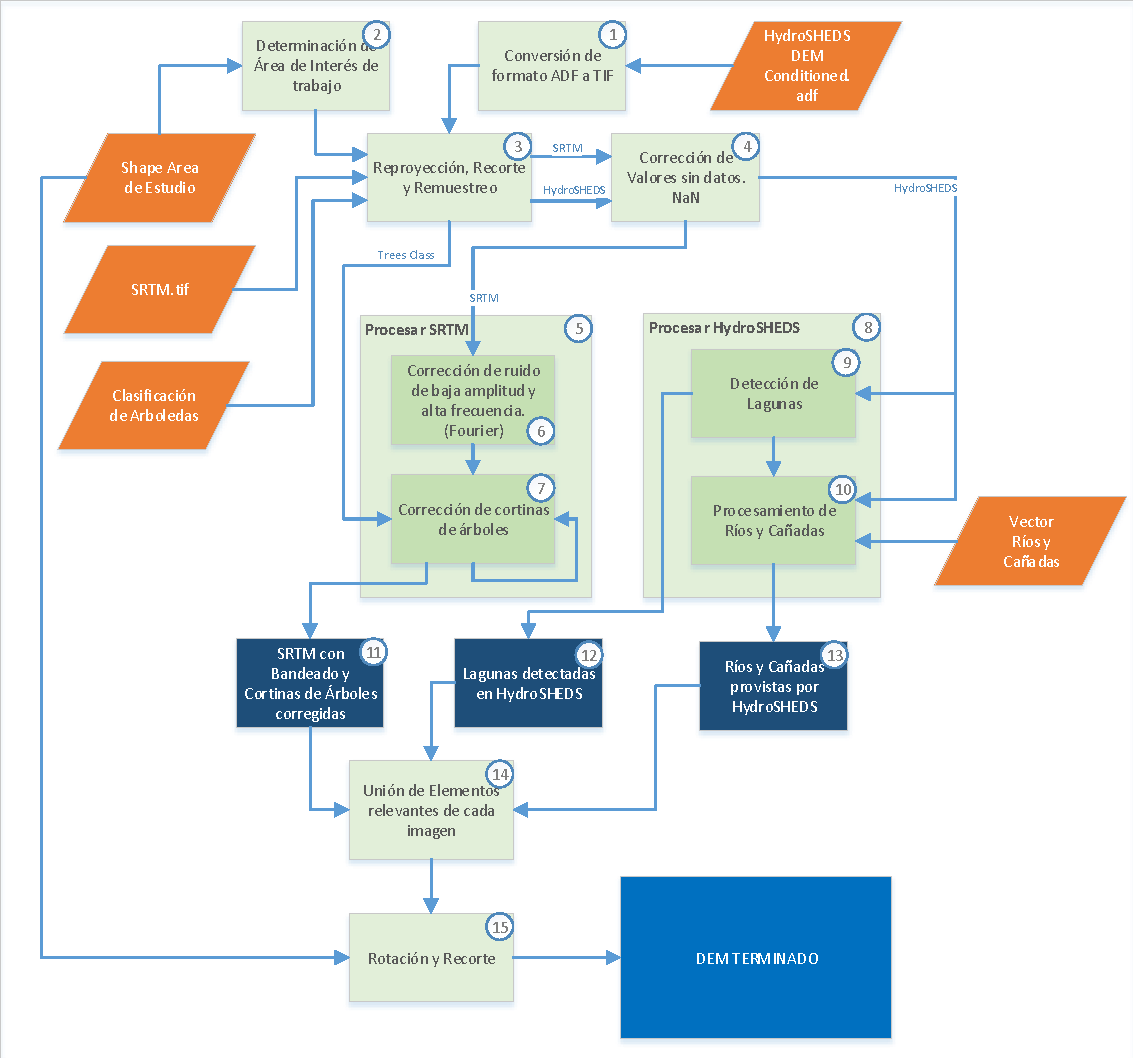
\includegraphics[width=1.0\textwidth]{imagenes/FlowChartsCompleto.pdf}
 \caption{Diagrama de flujo del procesamiento realizado el DEM para adecuación para usos hidrológicos.}
 \label{FlowCompleto}
\end{figure}


\begin{itemize}
	\item En color anaranjado se representan los datos de entrada necesarios para el procesamiento.
	\item En color verde claro se representan las funciones realizadas sobre los datos de entrada, mientras que en color verde un poco más oscuro se destacan subfunciones de las anteriores mencionadas, esto se destaca de esta manera debido a las claras diferencias de procesamiento, para una mejor comprensión. Estas operaciones además, son expandidas y es descripto posteriormente su funcionamiento interno. 
	\item En color azul oscuro se muestran los datos principales de salida, mientras que en azul más claro y al final, el producto de salida, resultado del procesamiento completo.
\end{itemize}

A continuación se describen brevemente los procesamientos realizados siguiendo la numeración de la figura \ref{FlowCompleto}. Una descripción más detallada se encuentra en las secciones posteriores.

\begin{enumerate}
	\item El DEM HydroSHEDS viene en formato adf (Application Definition File). Se convierte a formato tiff como primer paso de su procesamiento.
	\item A partir del shape del área de estudio que se asume es rectangular, se determina el área de estudio con la cual se trabajará casi en la totalidad del trabajo, esto es un área que sea paralela con respecto al ecuador y que contenga todo el área de estudio de entrada. Esto se realiza para no realizar una rotación con interpolaciones de valores de píxeles antes de cualquier procesamiento.
	\item El DEM HydroSHEDS ya en formato tiff, el DEM SRTM, y la clasificación de arboledas son reproyectadas, recortadas y remuestradas utilizando el archivo shape del área de interés procesado previamente. Esto se hace para tener una correspondencia entre los píxeles a procesar.
	\item Se corrigen los valores sin valor (NaN) de estos elementos.
	\item El DEM SRTM es procesado por separado del DEM HydroSHEDS.
	\item Se aplica a SRTM la corrección de ruido de baja amplitud y alta frecuencia.
	\item Luego de aplicada la corrección usando la transformada de Fourier se aplica a SRTM la corrección de cortinas de árboles.
	\item El DEM HydroSHEDS es procesado por separado del DEM SRTM.
	\item Se aplica a HydroSHEDS el algoritmo de detección de lagunas.
	\item Se rasteriza el vector de ríos y cañadas y teniendo como base HydroSHEDS se aplica el algoritmo de enrutamiento de ríos y cañadas.
	\item DEM SRTM corregido
	\item Se extraen de HydroSHEDS los valores que corresponden con lagunas detectadas
	\item Se extraen de HydroSHEDS los valores que corresponden con ríos y cañadas luego de procesados.
	\item Los elementos mencionados anteriormente se combinan en uno solo.
	\item Se aplica la rotación correspondiente con el shape original y se recorta.	
\end{enumerate}

\subsection{Clasificación de Arboledas}
\label{clasificacionArboledas}

Para poder disponer de uno de los datos de entrada necesarios para este trabajo se realizó una clasificación supervisada de las arboledas existentes en el área. Esta clasíficación se realizó de modo manual, debido a que su automatización extendería demasiado el alcance de este trabajo.

Los pasos realizados para lograr tal clasificación son descriptos a continuación.

\subsubsection{Datos de Entrada necesarios para la clasificación de arboledas}


\textbf{Imágenes Opticas Landsat}
\label{imagenesLandsat}

Para la clasificacion se escogen imágenes Landsat que contienen el área de estudio. Se busca en el sitio EarthExplorer perteneciente al USGS de los Estados Unidos (https://earthexplorer.usgs.gov/) el path y el row correspondiente. En este caso es el path: 228, row: 83 Fig. \ref{footprintLandsat}. Se realiza el pedido del producto OLI/TIRS HigherLevel ya que provee productos de reflectancia de superficie. Los productos de reflectancia de superficie proporcionan una estimación de la reflectancia espectral de la superficie, como si hubieran sido medidos a nivel del suelo en ausencia de dispersión atmosférica o absorción. \cite{OLITIRS} 

\begin{figure}[!htb]
   \centering      
   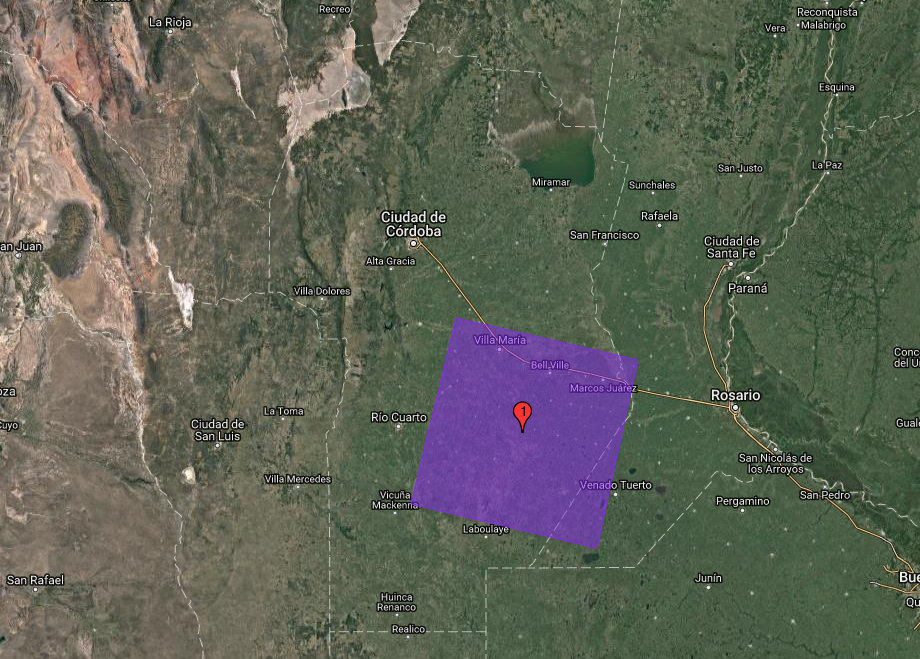
\includegraphics[width=0.85\textwidth]{imagenes/FootLandsat228_83.jpg}
 \caption{Huella del path y row de las imágenes Landsat 8 elegidas para la clasificación}
 \label{footprintLandsat}
\end{figure}

Se buscaron imágenes de diferentes épocas del año, para que la clasificación sea más representativa. Las imágenes utilizadas para esta clasificación corresponden a las fechas:

\begin{itemize}	
	\item 23 de Agosto de 2016
	\item 13 de Diciembre de 2016
	\item 20 de Abril de 2017
\end{itemize}

\textbf{Datos de Referencia}

Se cuenta con datos de verdad disponibles correspondientes a cultivos de la zona (Figura \ref{DatosDeVerdadCultivos}). Estos datos son polígonos en formato shape cuyos atributos contienen a que tipo de cultivo pertenece cada polígono.

\begin{figure}[!htb]
   \centering      
   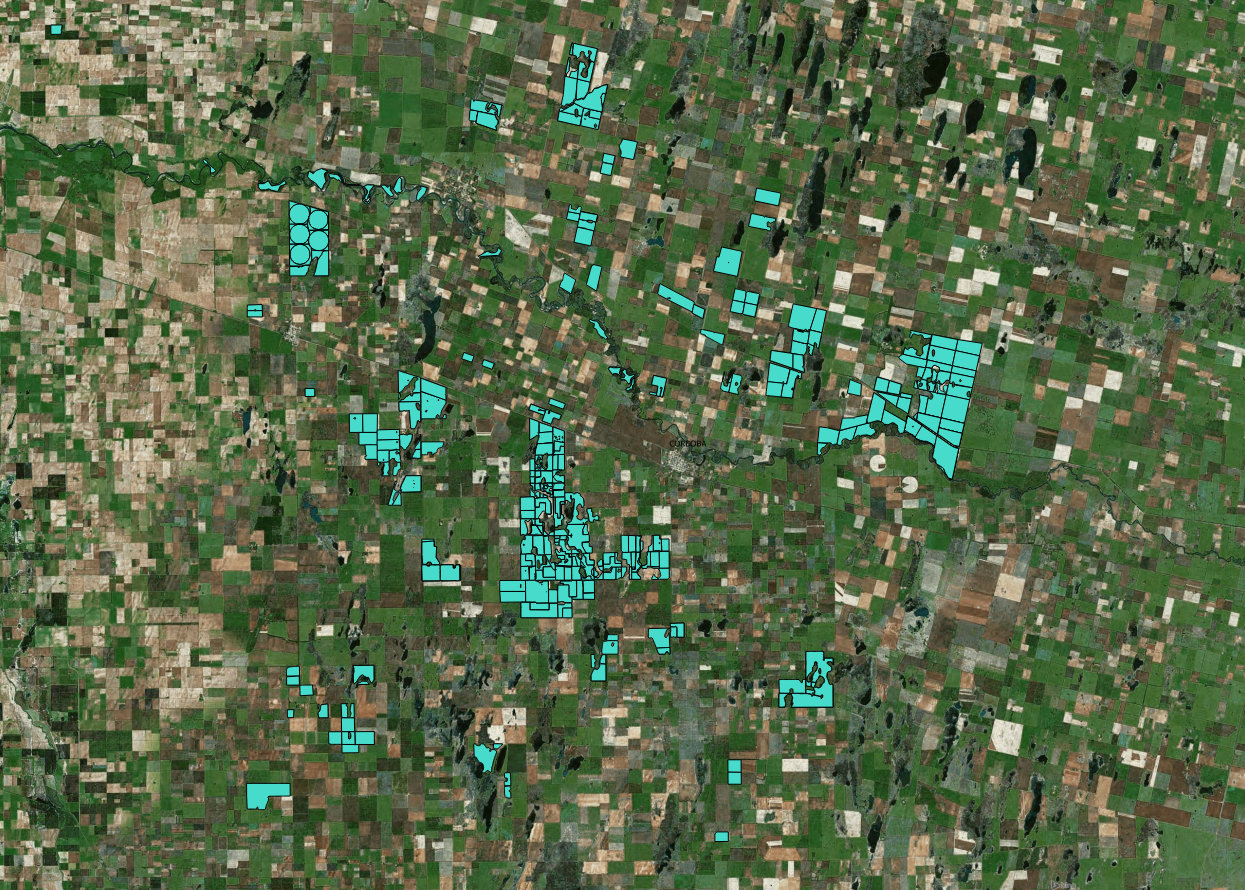
\includegraphics[width=0.85\textwidth]{imagenes/DatosDeVerdadCultivos.jpg}
 \caption{Datos de Verdad de Cultivos sobre imagen satelital perteneciente a Bing Aerial}
 \label{DatosDeVerdadCultivos}
\end{figure}

Además, utilizando la herramienta de información geográfica QGIS se crearon polígonos correspondientes a árboles, Figura \ref{ShapeArboles}. Esta tarea fue realizada cargando el complemento de mapas libre Bing que tiene alta resolución de imagen superponiéndolo con una de las bandas de las imágenes Landsat antes mencionadas. También fueron identificados ríos y lechos de río.

\begin{figure}[!htb]
   \centering      
   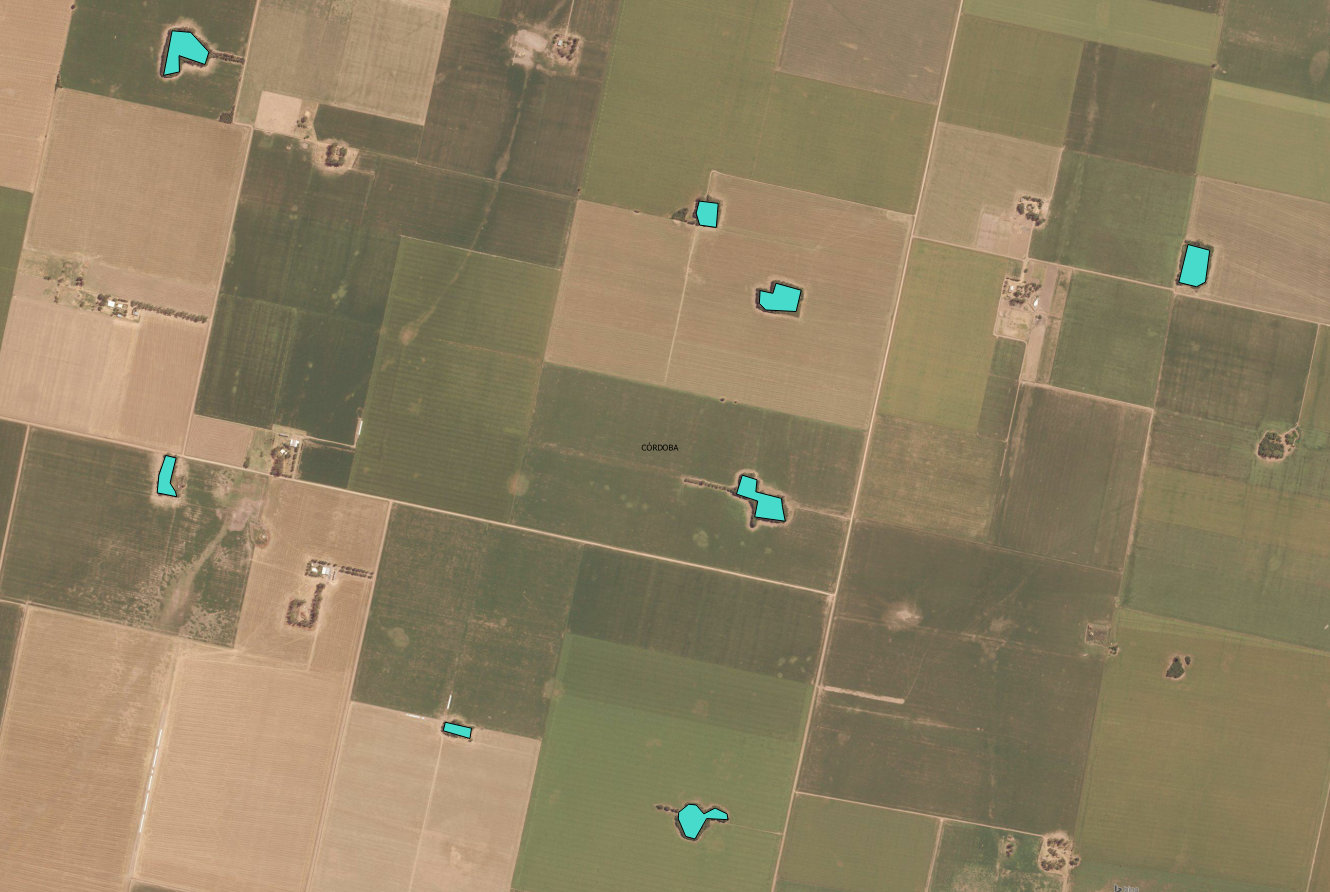
\includegraphics[width=0.85\textwidth]{imagenes/ShapesArboles.jpg}
 \caption{Identificación de arboledas en área de estudio}
 \label{ShapeArboles}
\end{figure}

\subsubsection{Creación del stack de imágenes}

Con estos datos a disposición se creo un stack de las bandas 2, 3, 4, 5 de las imágenes mencionadas en la sección \ref{imagenesLandsat}.

\subsubsection{Clasificación}

El complemento de clasificación de QGIS llamado Dztesaka \cite{dzetsaka} es utilizado para la clasificación. El modelo de clasificación contenido en el complemento y utilizado es Gaussian Mixture Model (Rasmussen 2000). El complemento Dzetsaka utiliza aleatoriamente la mitad de los datos de verdad para entrenamiento del modelo y la otra mitad para clasificación de la imagen.


\subsection{Datos de Entrada}

\begin{itemize}
\item Archivo SRTM en formato .tif descargado del sitio USGS
\item Archivo HydroSHEDS en formato .adf descargado del sitio USGS
\item Archivo en formato shape (.shp). Este debe ser rectangular para poder llegar a una rasterización correcta de la imagen. Puede tener cierto angulo de inclinación, debe ser conocido.
\item Clasificación de Arboledas. Debe ser una imagen tif cuyos valores de píxeles deben ser 1 (presencia de árboles) o 0 (ausencia de árboles).
\item Vector de Ríos y Cañadas: Debe estar recortado para la zona que cubre el área de estudio y que es paralela horizontalmente con los paralelos geográficos.
\end{itemize}


\subsubsection{DEM SRTM en formato TIF}

DEM SRTM en formato TIF. Este dato de entrada fue descripto de manera detallada en la sección \ref{SRTMDefincion}, puede descargarse de manera gratuita del sitio WEB del Servicio Geológico de Estados Unidos (USGS) del siguiente link  \hyperref[http://srtm.csi.cgiar.org/SELECTION/inputCoord.asp]{``http://srtm.csi.cgiar.org/SELECTION/inputCoord.asp"}.


\subsubsection{DEM HydroSHEDS Conditioned en formato ADF}


DEM en formato ADF acondicionado para usos hidrológicos. Este dato de entrada fue descripto de manera detallada en la sección \ref{HydroSHEDSDef}, puede descargarse de manera gratuita del sitio WEB del USGS, por medio del siguiente enlace  \hyperref[http://hydrosheds.cr.usgs.gov/dataavail.php]{``http://hydrosheds.cr.usgs.gov/dataavail.php"}. Cada uno de los mosaicos de este tipo de DEM se corresponden geográficamente con los DEM SRTM.


ADF es un formato de datos de trama interno utilizado por productos de ESRI como ArcGIS, ArcView y ArcInfo Workstation. Almacena datos espaciales como una cuadrícula binario y es uno de varios archivos ADF que en conjunto constituyen la red total. Se utiliza para representar objetos espaciales geográficas o de otro tipo, tales como mapas y las características del mapa.

A partir de este dato de entrada se obtendrán las regiones del área de estudio correspondientes a lagunas y cañadas.

\begin{figure}[!htb]
   \centering      
   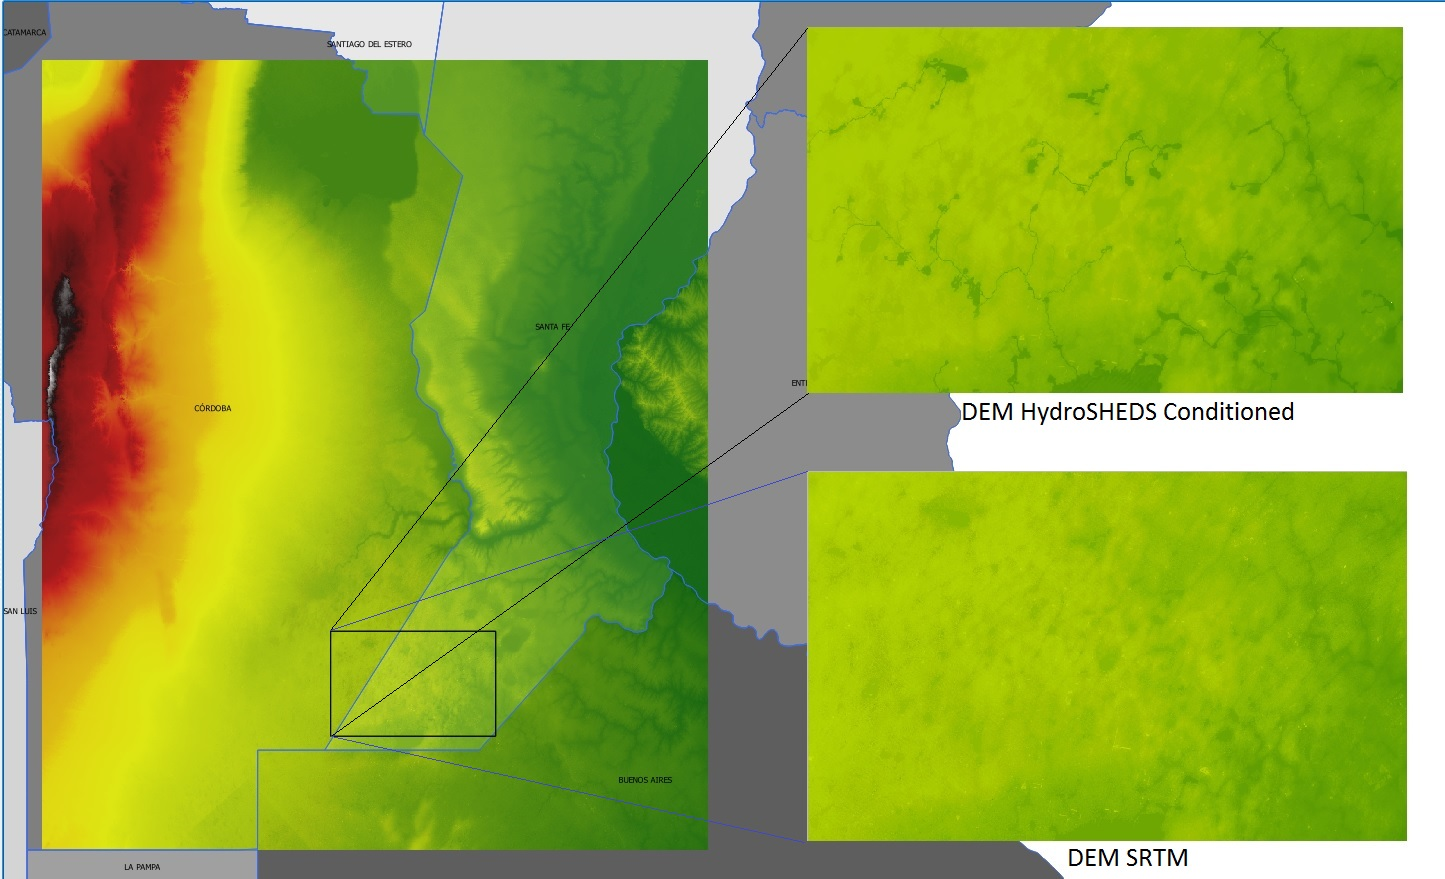
\includegraphics[width=1.0\textwidth]{imagenes/ComparacionHydroSHEDSSRTM.jpg}
 \caption{Para la misma zona, una comparación visual entre el DEM HydroSHEDS Conditioned y el DEM SRTM. El DEM HydroSHEDS provee mejor definición de cañadas.}
 \label{HydroSHEDSSRTM}
\end{figure}


\subsubsection{Archivo en formato Shape de Área de Estudio}

Teniendo en cuenta que se pretende realizar el procesamiento del DEM para una determinada zona de interés, se debe proveer un elemento que indique cual es esta zona de interes. Ésta debe proveerse por medio de un archivo shape (SHP, Shapefile). Debe ser de forma rectangular. En caso de tener cierta rotación con respecto a los paralelos, se debe conocer esta rotación así como proveerla. 

En la figura \ref{HydroSHEDSSRTM} se puede observar el DEM SRTM correspondiente a un mosaico que cubre gran parte de la provincia de Córdoba y conteniendo el shape del área de estudio. Todo el trabajo fue desarrollado utilizando el área de estudio expuesta en la figura.




\subsubsection{Clasificación de Arboledas}

El usuario puede proveer su propia clasificación realizada con la metodología que prefiera proveyendo como dato de entrada una máscara de las arboledas identificadas. Para este trabajo se utilizó la clasificación de arboledas descripta en la sección \ref{clasificacionArboledas}


\subsubsection{Ríos y Cañadas}
\label{vectorRiosArea}

Es importante proveer una imagen de máscara de ríos y cañadas debido a que es necesaria para extraer esta información de manera automática del DEM provisto por HydroSHEDS. HydroSHEDS provee buena información de datos de altura para estas áreas. Contando con una buena máscara se identificarán con facilidad y se podrá combinar luego con el DEM SRTM.

Los datos de ríos y cañadas de la zona también son provistos por el sitio de HydroSHEDS y pueden ser descargados libremente de \cite{hydroShedsSite}. Fue descargado el producto correspondiente a Sudamérica. Estos datos son provistos en formato vectorial de líneas. A esta capa vectorial se le aplicó un recorte de un rectángulo horizontal que contiene en su totalidad al área de estudio (Figura \ref{areaestudiorios}).


\begin{figure}[!htb]
   \centering      
   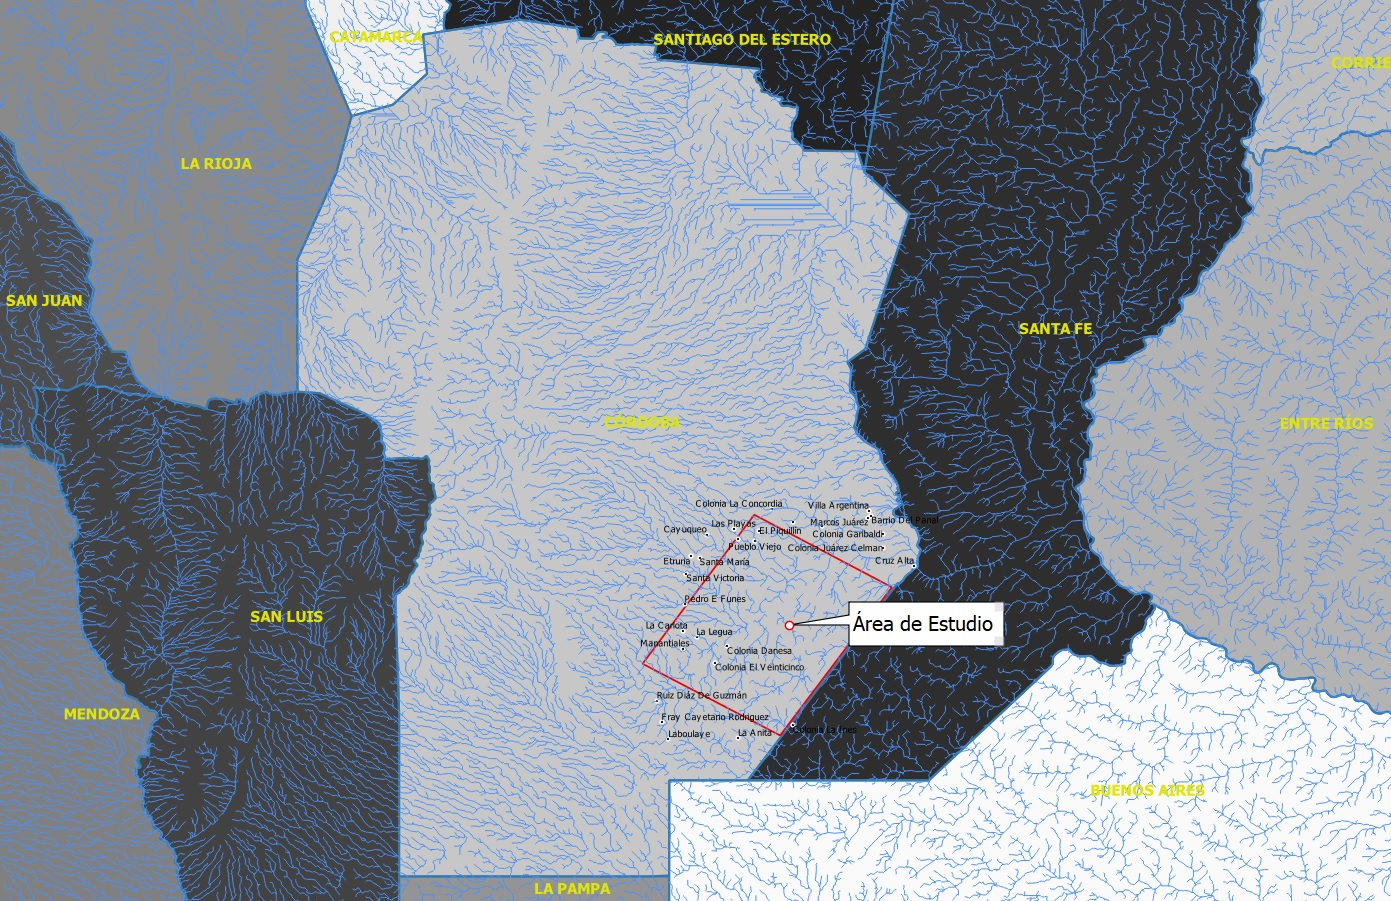
\includegraphics[width=1.0\textwidth]{imagenes/areaestudiorios.jpg}
 \caption{Recorte del área de estudio aplicada a capa vectorial de rios.}
 \label{areaestudiorios}
\end{figure}

\subsection{Procesamiento y operaciones a SRTM y HydroSHEDS}


\subsubsection{Reproyección}

Se realizó una reproyección de la imagen al Marco de Referencia Geodésico Nacional POSGAR 94. Esto es conveniente hacer porque es el sistema de proyección oficial de Argentina.

\subsubsection{Recorte y Remuestreo}

Una vez que la imagen fue reproyectada y con el archivo shape rectangular del área de estudio a disposición, ee puede proceder a realizar el recorte del área de estudio. Se debe recordar que el área abarcada por el archivo de polígono se debe encontrar dentro del área comprendida por el DEM en formato tif. Figura \ref{SRTMAndShape}.

Algo a tener en cuenta es que los píxeles contenidos no abarcan áreas cuadradas, esto se debe a que cada píxel comprende 3 arco-segundos en coordenadas de latitud-longitud. Teniendo en cuenta las latitudes en las cuales se trabaja, el lado vertical de cada píxel es mayor que los horizontales. Este efecto es logrado al hacer una proyección del DEM sobre el terreno, por lo que fue necesario realizar un remuestreo de los píxeles contenidos en la imagen.

Por medio de la herramienta $gdal\_warp$ comprendida en $gdal$ se puede realizar:

\begin{itemize}
\item Recorte de área de un archivo tif usando un archivo shape contenido dentro del tif.
\item Especificación en el tamaño de cada píxel, de esta forma se realiza un remuestreo de la imagen utilizando el método del vecino más cercano. El tamaño es establecido en 90 metros de lado.
\item El tipo de dato es convertido a flotante de 32 bits.
\end{itemize}

Como resultado se obtiene una imagen en formato tif rectangular perpendicular al norte. En el caso en que el shape que se provee como dato de entrada tenga algún grado de inclinación, la imagen recortada puede tener huecos en los bordes para completar el cuadrado que contiene al área definida por el shape. Estos "`huecos"' son considerados por gdal como valores NaN a los cuales les asigna el menor valor posible (-32768).

Se debe tener en cuenta que la imagen por si misma puede traer píxeles con valores NaN, por errores propios de la imagen provista por USGS.

\subsubsection{Corrección de píxeles sin datos. (valores NaN)}

La librería GDAL de python, con la cual se realizan la mayoría de los procesamientos, asigna el menor valor posible, según de que tipo sean, cuando encuentra un valor NaN.
Si bien es bastante claro que siempre es necesaria la corrección de los valores NaN en píxeles dentro de la imagen, esta corrección se hace más notable antes de realizar una rotación de la imagen, esto se debe a que en la rotación se realiza una interpolación con píxeles vecinos y valores extremadamente bajos, lo cual puede dar lugar a la introducción de errores.

Para determinar el valor que obtendrá el píxel a corregir solo se deben tener en cuenta los vecinos cuyos valores sean positivos, teniendo en cuenta la naturaleza de los valores del DEM, se asume que valores negativos son valores no deseados. De esta manera se corregirán los valores de píxeles con valores NaN dentro del área de estudio o en los bordes de la misma.


\subsection{Procesamiento a SRTM}

\subsubsection{Corrección de ruido de baja amplitud y alta frecuencia. (Fourier)}
\label{correccionfourier}



El DEM SRTM provisto por USGS trae un bandeado inherente (Figura \ref{SinFourier}), similar al que se observa para el DEM de Hydroshed mostrado en la figura \ref{HSHEDSPaleta}, el cual debe ser corregido si se quiere utilizar con fines hidrológicos. Es importante tener en cuenta que el DEM al cual se le debe corregir tal bandeado puede haber sido rotado, por lo tanto la orientación del bandeado puede variar y por consecuencia los valores a corregir en la transformada de Fourier, dependiendo la rotación aplicada y el tamaño de la imagen.

\begin{figure}[!htb]
   \centering      
   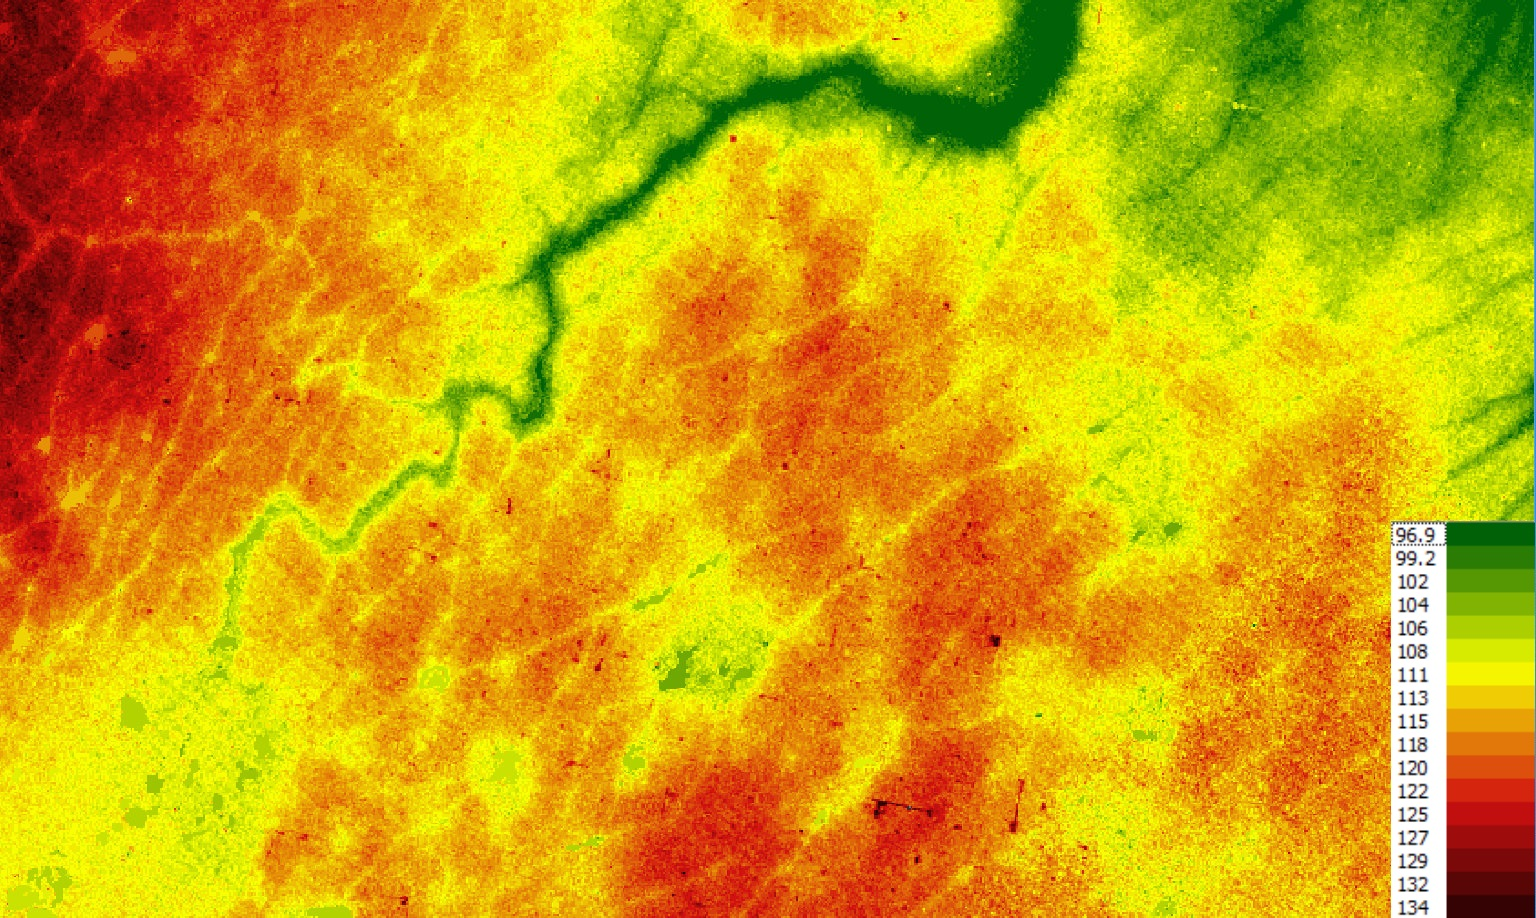
\includegraphics[width=0.85\textwidth]{imagenes/SRTMSinFourier.jpg}
 \caption{Sección de DEM SRTM con bandeado inherente. Se aplicó una paleta de colores en donde se pueda destacar el bandeado.}
 \label{SinFourier}
\end{figure}


Es por eso que es deseable que la corrección de tal bandeado usando la transformada de Fourier detecte de manera automática las frecuencias de Fourier a corregir. La secuencia de pasos que fue desarrollada para llevar a cabo tal corrección respeta el siguiente diagrama de flujo (figura \ref{DiagramaFourier} y es descripta a continuación:


\begin{figure}[!htb]
   \centering      
   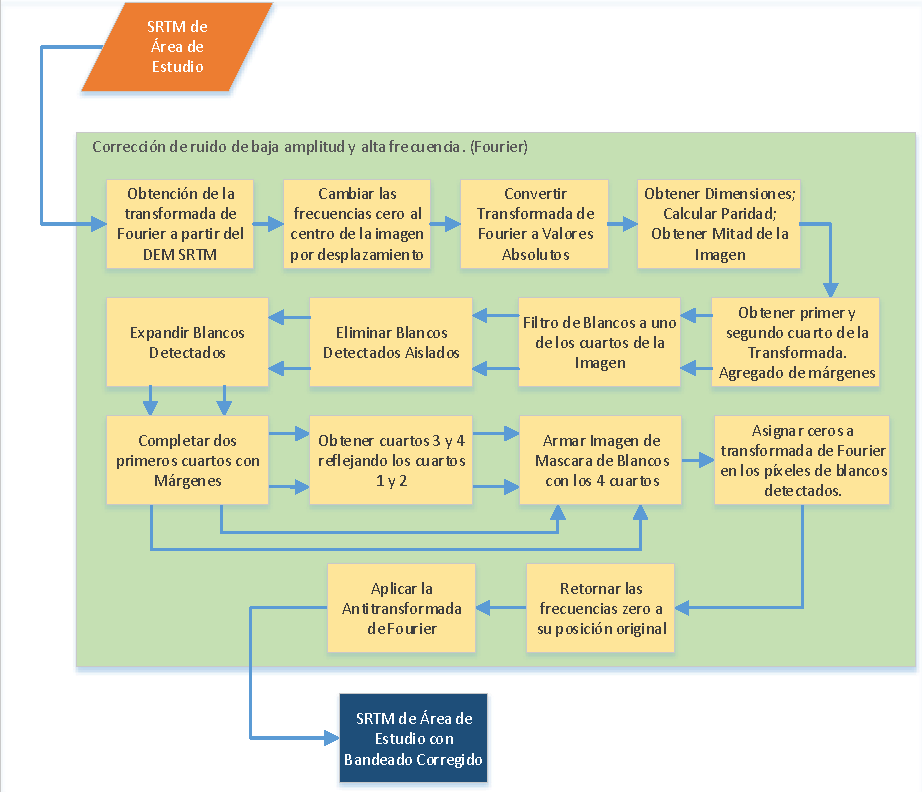
\includegraphics[width=0.85\textwidth]{imagenes/DiagramaFourier.pdf}
 \caption{Diagrama de flujo de ejecución de pasos para llevar a cabo la corrección de bandeado usando la transformada de Fourier.}
 \label{DiagramaFourier}
\end{figure}


\textbf{Obtención de la transformada de Fourier a partir del DEM SRTM}

Como primer paso se debe obtener la transformada de Fourier de la imagen a corregir (González \textit{et al.} 1993). Esto se hace de manera muy simple con funciones incluidas en librerías matemáticas, se obtiene como resultado la imagen que podemos observar en la figura \ref{FourierNoCentrada}:

\begin{figure}[!htb]
   \centering      
   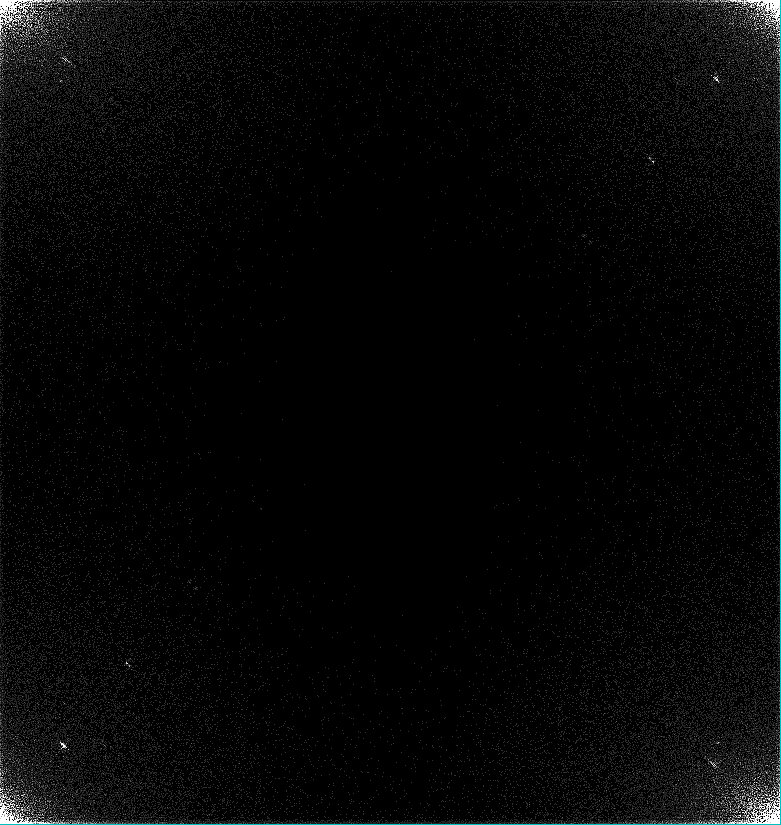
\includegraphics[width=0.45\textwidth]{imagenes/FourierNoCentrada.jpg}
 \caption{Espectro de frecuencias de Fourier en dos dimensiones.}
 \label{FourierNoCentrada}
\end{figure}


\textbf{Cambiar las frecuencias cero al centro de la imagen por desplazamiento}

La transformada de Fourier representa el espectro centrado de frecuencia de Fourier (Figura \ref{FourierTransform}). Si hacemos zoom sobre esta imagen de frecuencias centrada podemos observar más claramente los blancos que deben ser corregidos (figura \ref{ZoomFourierTransformBlancos}).

\begin{figure}[!htb]
   \centering      
   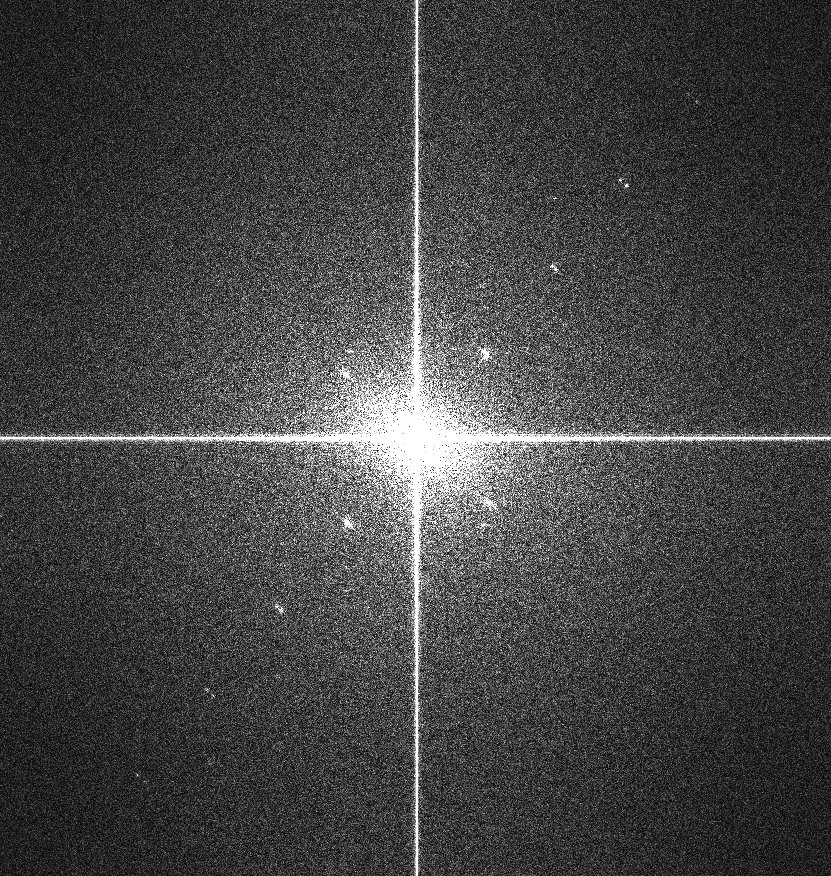
\includegraphics[width=0.45\textwidth]{imagenes/FourierTransform.jpg}
 \caption{Espectro de frecuencias de Fourier centrada.}
 \label{FourierTransform}
\end{figure}

\begin{figure}[!htb]
   \centering      
   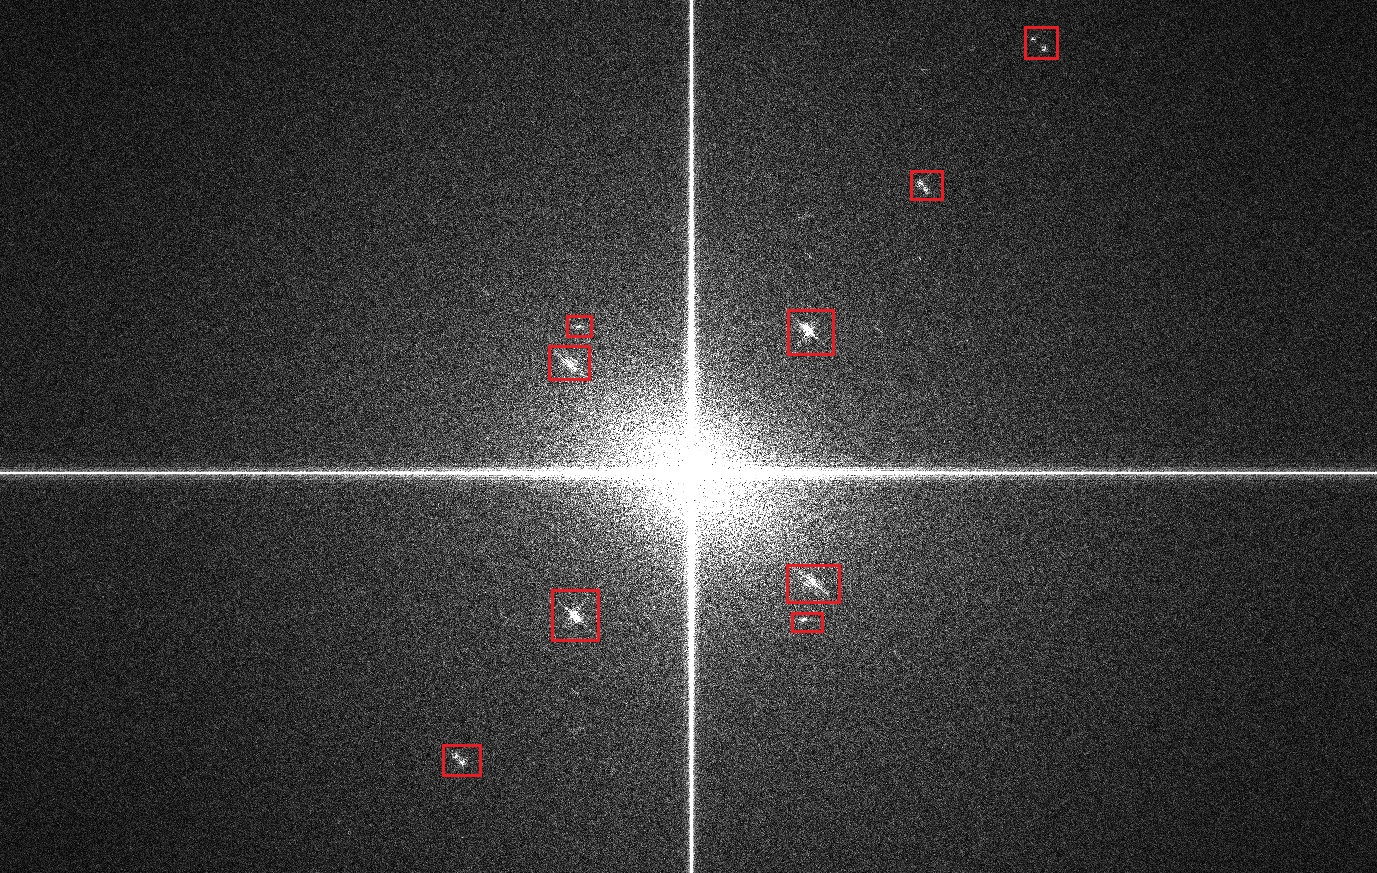
\includegraphics[width=0.85\textwidth]{imagenes/ZoomFourierTransformBlancos.jpg}
 \caption{Zoom sobre la imagen del espectro de frecuencias de Fourier centrada en donde se pueden observar, destacados con un rectángulo rojo, los blancos que se deben corregir.}
 \label{ZoomFourierTransformBlancos}
\end{figure}

\textbf{Convertir Transformada de Fourier a Valores Absolutos}

Teniendo en cuenta que la imagen de transformada de Fourier esta compuesta por números complejos, será más simple obtener el valor absoluto de este numero complejo para simplificar el procesamiento. Por lo tanto se aplica esta operación sobre la imagen de frecuencias.

\textbf{Extracción de los cuartos}

El próximo paso consiste en detectar de manera automática los blancos a corregir en la imagen de frecuencias.



La cruz central de la imagen que representa debe ser excluida de la detección de blancos a corregir ya que ofrece valores tanto o más altos que los blancos buscados. Si dividimos la imagen por la mitad, tanto horizontal como verticalmente obtenemos cuatro cuartos determinados por esta cruz central y los numeramos como se puede ver en la figura \ref{CuartosFourier} 

\begin{figure}[!htb]
   \centering      
   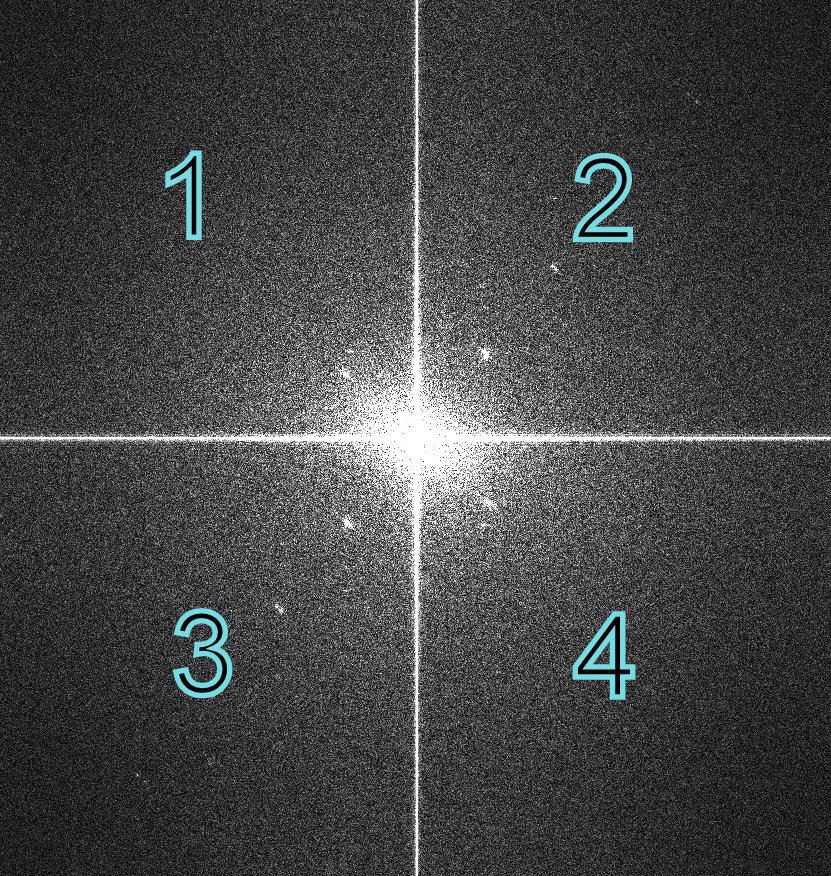
\includegraphics[width=0.85\textwidth]{imagenes/CuartosFourier.jpg}
 \caption{Enumeración de los cuartos en los que dividimos la imagen de frecuencias de Fourier para su procesamiento.}
 \label{CuartosFourier}
\end{figure}

Podemos observar que el primer cuarto es simétrico con respecto al cuarto, espejado diagonalmente, es decir horizontal y verticalmente, así como el segundo se corresponde con el tercero, espejado también por la diagonal.

Con esta información, se realiza la detección de blancos para los dos primeros cuadrantes por separado para luego espejarlos y obtener los cuadrantes tres y cuatro. Se debe destacar que, dada la independencia en la detección de blancos para los dos primeros cuartos, se pudo aplicar paralelismo al procesamiento, lo que logra una mayor eficiencia en la ejecución.

Para esto se realizan recortes de estos dos primeros cuadrantes dejando fuera también los valores que corresponden con las líneas centrales (que poseen altos valores también) por lo que se adopta un margen de 10 píxeles para excluir las líneas centrales (Figuras \ref{firstQuarter} y \ref{secondQuarter}).

\begin{figure}[!htb]
   \begin{minipage}{0.48\textwidth}
			\centering
			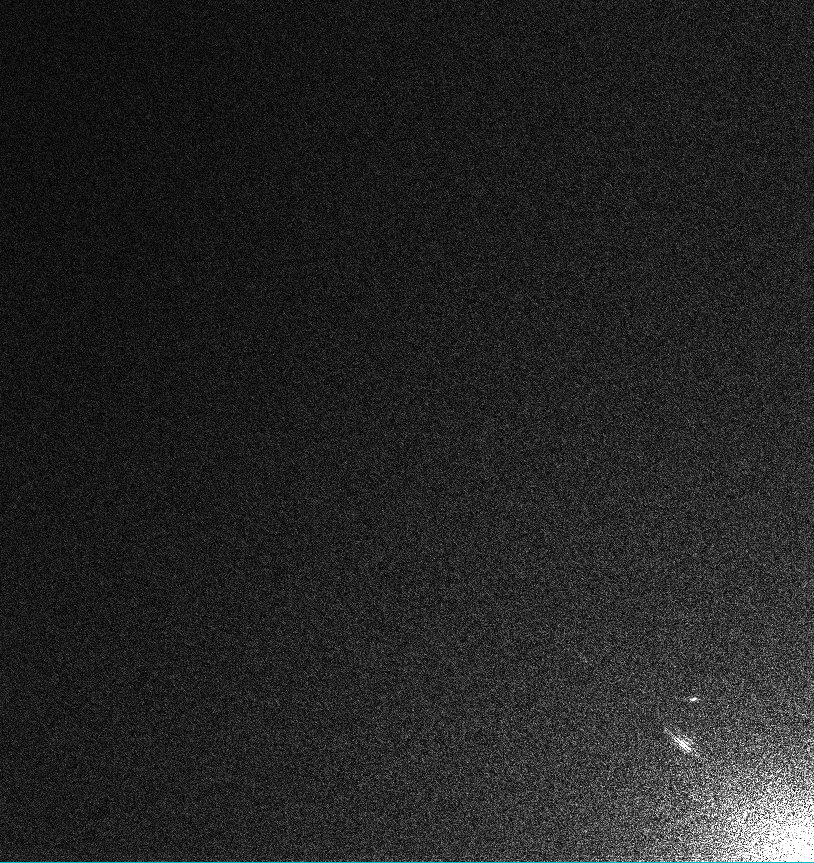
\includegraphics[width=1.0\linewidth]{imagenes/fstQuarterFourier.jpg}
			\caption{Primer cuarto extraído de la imagen de frecuencias de Fourier.}
			\label{firstQuarter}
   \end{minipage}\hfill
   \begin {minipage}{0.48\textwidth}
			\centering
			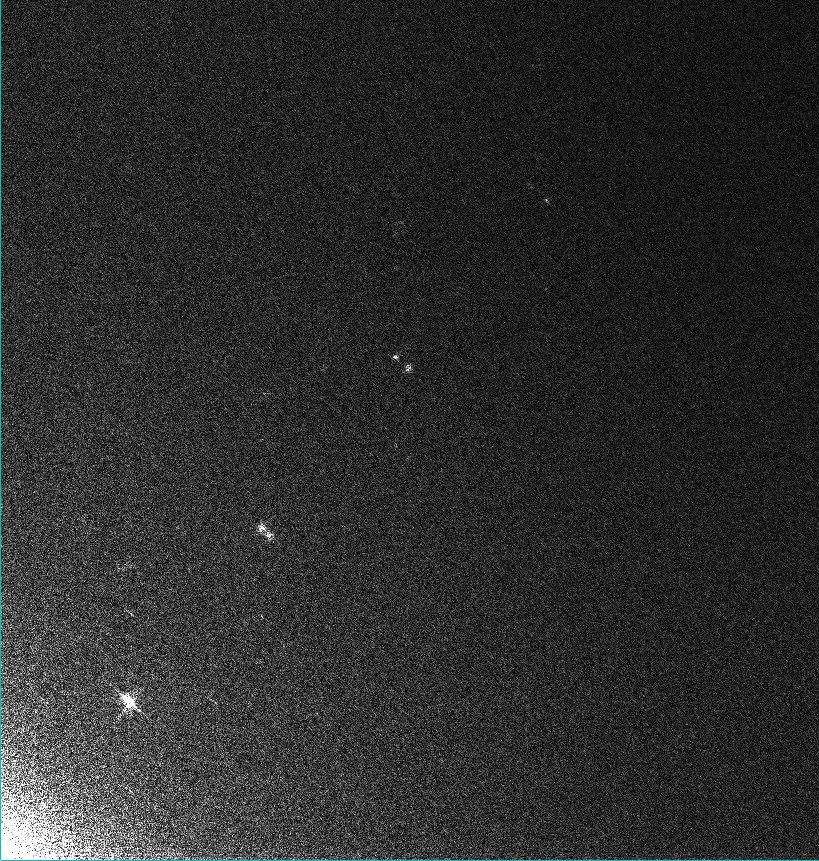
\includegraphics[width=1.0\linewidth]{imagenes/sndQuarterFourier.jpg}
			\caption{Segundo cuarto extraído de la imagen de frecuencias de Fourier.}
			\label{secondQuarter}
   \end{minipage}
\end{figure}

Es importante tener en cuenta la paridad de las dimensiones de la imagen (cantidad de píxeles horizontales y verticales), ya que es necesario al momento de recortar y luego rearmar la imagen. En el caso que sea cantidad par se divide por la mitad y cada parte obtiene la mitad de los píxeles, en el caso de que sea impar también se divide por la mitad, se toma la parte entera de píxeles de la división y se tiene en cuenta que la cantidad es impar para agregar luego una linea de píxeles extra.

Es por eso que este proceso tiene varias partes:

\begin{itemize}
	\item Obtención dimensiones de la imagen.
	\item Cálculo de paridad de la dimensión.
	\item Obtención de la mitad de la imagen.
	\item Determinación de primer y segundo cuarto.
	\item Agregado de márgenes a los cuartos.
\end{itemize}

\textbf{Algoritmo de detección de blancos}
Una vez obtenidas las áreas correspondientes a los dos primeros cuartos, se aplica el algoritmo de detección de blancos para cada una de ellas.

\textbf{Filtro de Blancos:} El filtro consta de una ventana de vecinos móviles de 55x55, en este caso sería una ventana "`hueca"' ya que son omitidos los píxeles cercanos al núcleo hasta una distancia de 5 píxeles de lado. Figura \ref{filtroBlancosFourier}

\begin{figure}[!htb]
   \centering      
   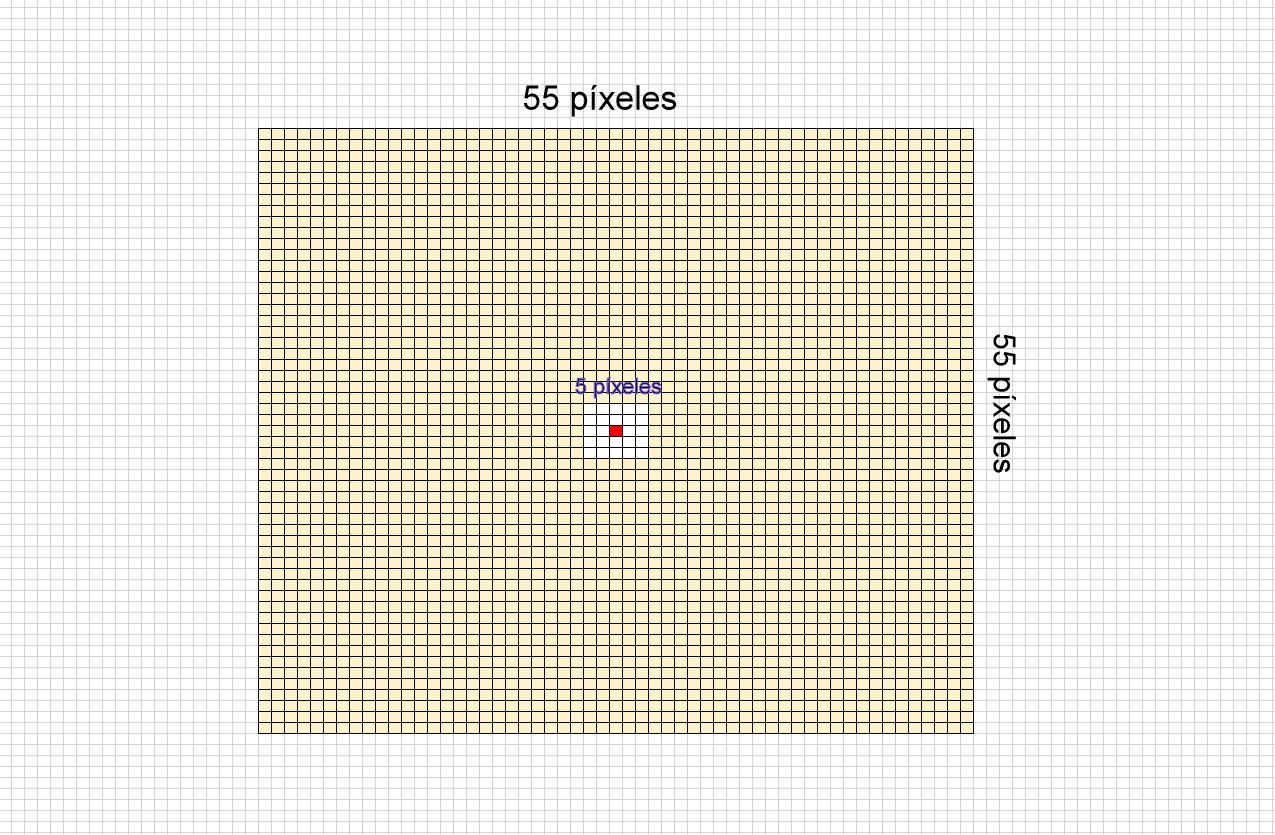
\includegraphics[width=0.85\textwidth]{imagenes/filtroBlancosFourier.jpg}
 \caption{Esquema de ventana de filtro de blancos de 55x55 con un hueco de 5x5.}
 \label{filtroBlancosFourier}
\end{figure}

Analizando manualmente los valores de los píxeles de tales blancos (Figura \ref{ZoomFourierTransformBlancos}) se pudo determinar que, tienen valores que exceden hasta cuatro veces más que el valor de sus \textbf{vecinos} (vecinos adyacentes dentro en un radio de distancia de veinte píxeles). 

\subsubsubsection{Condición de pertenencia a la máscara - Filtro: } El filtro aplicado es un kernel de 50x50 excluyendo a los 5x5 vecinos más cercanos al centro del kernel. Se calcula el valor medio de todo el conjunto de vecinos. Se incluirá a la máscara de resultado a los píxeles del centro de la ventana si su valor es por lo menos \textbf{cuatro veces más grande} que la media de los vecinos dentro de la ventana de 50x50.

En función de este análisis se desarrolló el filtro y el algoritmo que lo ejecuta. Este algoritmo consta de tres partes fundamentales:

\textbf{Iteraciones sobre la imagen con el filtro definido:}

En cada iteración de aplicación del filtro dos resultados son retornados y actualizados para la próxima iteración:

\begin{itemize}
\item La máscara con los píxeles que cumplen la condición del filtro. Esta máscara es sumada a la máscara calculada en el paso anterior, o a la inicial (todos ceros) en caso que sea la primera iteración, por lo cual se irán acumulando los blancos detectados. De esta manera la cantidad de blancos detectados va creciendo en cada iteración.
\item La imagen de entrada del filtro en donde los píxeles que fueron detectados como blancos se les asignó el valor cero.  Esto se hace porque si fue agregado a la máscara, implica que es un valor alto y, al asignarle el valor cero, no interferirá en el calculo de valores medios para iteraciones posteriores.
\end{itemize}

Se realizaron pruebas con diversos valores de cantidad de iteraciones. En algunos casos se necesitaron hasta 5 iteraciones para detectar todos los blancos presentes, mientras que en las últimas pruebas alcanzó con 2 iteraciones, de igual manera este valor se dejó establecido en 5 para estar más seguro de la detección completa.

Como salida luego de las iteraciones definidas se obtiene una imagen con ceros donde no se detectaron blancos, y unos donde se satisface la condición de la máscara.


\textbf{Eliminar Blancos Detectados Aislados} Debido a que los blancos a detectar suelen ser un conjunto de puntos agrupados, es probable que, ademas de los blancos detectados, se detecten puntos sueltos que satisfagan la condición del filtro, pero que no correspondan a valores que se deben corregir en la transformada de Fourier. Estos son falsos positivos por lo que se definió una función para la eliminación de estos puntos aislados. Básicamente, si un píxel perteneciente a la máscara tiene todos sus vecinos dentro de una ventana de 13x13 con valores cero, dicho píxel debe ser quitado de la máscara. 

% Esquema con el filtro que se usa.

\textbf{Expandir Blancos Detectados:} Una vez obtenida la máscara, se aplica un filtro de dilatación de 13x13 sobre los píxeles detectados ((González \textit{et al.} 1993)), para así garantizar la cobertura del conjunto de vecinos que determinan un blanco en la imagen de la transformada de Fourier. Con este filtro se logra expandir al área de las áreas de la imagen con valor 1.

Luego de la detección de blancos, eliminación de puntos aislados y el filtro de dilatación se obtiene una máscara de blancos para los cuartos aplicada como se puede observar en las figuras \ref{firstQuarterMask} y \ref{firstQuarterMask}


\begin{figure}[!htb]
   \begin{minipage}{0.48\textwidth}
			\centering
			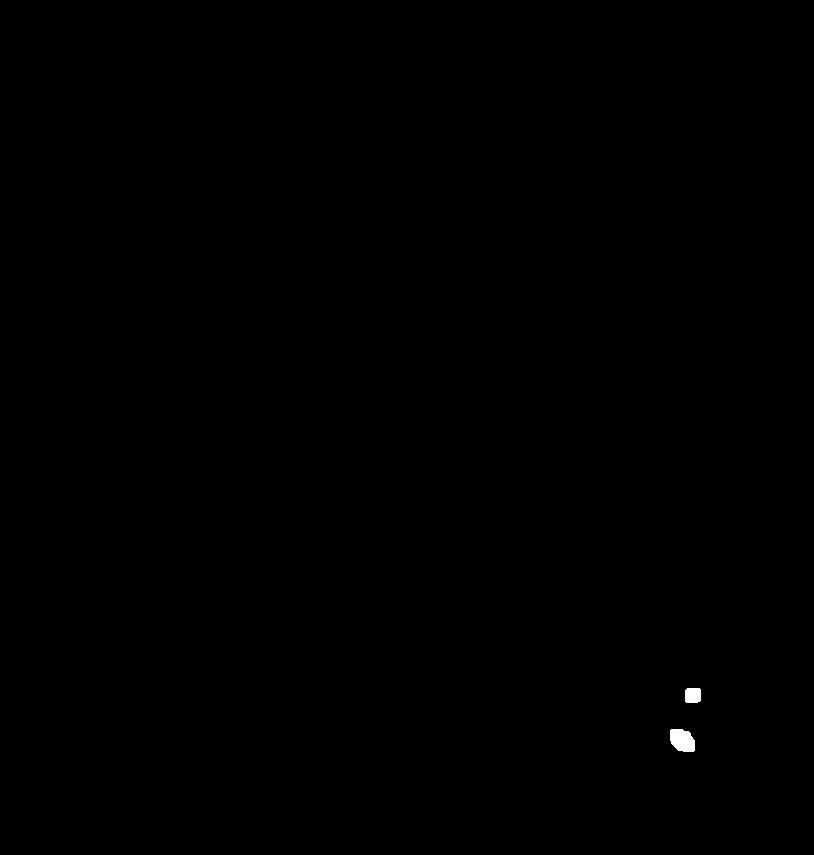
\includegraphics[width=1.0\linewidth]{imagenes/fstQuarterFourierMask.jpg}
			\caption{Blancos detectados en primer cuarto con eliminación de puntos aislados y filtro de dilatación de 13x13.}
			\label{firstQuarterMask}
   \end{minipage}\hfill
   \begin {minipage}{0.48\textwidth}
			\centering
			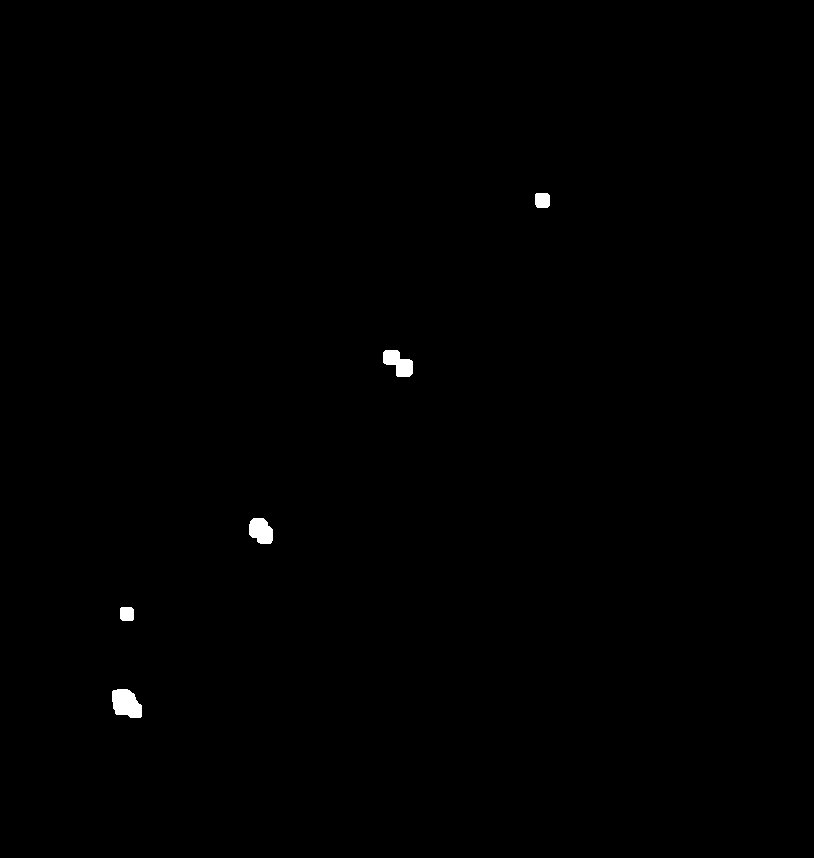
\includegraphics[width=1.0\linewidth]{imagenes/sndQuarterFourierMask.jpg}
			\caption{Blancos detectados en primer cuarto con eliminación de puntos aislados y filtro de dilatación de 13x13.}
			\label{firstQuarterMask}
   \end{minipage}
\end{figure}



\textbf{Paralelización de detección de blancos en cuadrantes}

Teniendo en cuenta el nivel de procesamiento de este filtro debido a:

\begin{itemize}
	\item Una ventana del kernel de 50x50 por cada píxel de la imagen.
	\item Cálculo de la media de los píxeles de esta ventana, por cada píxel y por la cantidad de vecinos mencionada.
	\item De 2 a 5 iteraciones de paso del filtro por cada cuarto.
\end{itemize}	

y teniendo en cuenta además que la detección de blancos en los cuadrantes uno y dos es independiente, se pensó conveniente paralelizar computacionalmente la ejecución de estas partes del código. Por lo tanto se ejecutan al mismo tiempo la detección de blancos en el cuarto uno como la detección de blancos en el cuarto dos. Esto requiere más trabajo del procesador, pero hace más eficiente la ejecución del algoritmo.


\subsubsubsection{Obtención de los cuadrantes 3 y 4, y armado de la imagen completa}

El algoritmo mencionado anteriormente es aplicado a los cuadrantes 1 y 2. Y se obtiene como resultado, las máscaras 1 y 2. Recordemos que a estos cuadrantes se les han recortado las franjas correspondientes con los bordes que limitan con las mitades de la imagen, tanto horizontal como verticalmente.

\textbf{Agregado de márgenes:} Es por eso que antes de realizar el espejado diagonalmente para obtener los cuadrantes 3 y 4 se deben completar estas franjas, en particular con valores 0, ya que en estas partes de la imagen no se encuentran blancos que indiquen correcciones.

\textbf{Obtención de cuartos 3 y 4 reflejando los cuartos 1 y 2:} Una vez obtenidos los cuadrantes 1 y 2 completos con los márgenes se puede realizar el espejado horizontal y vertical de ambos cuartos para obtener los opuestos diagonalmente. Figuras \ref{thirdQuarterMask} y \ref{fourthQuarterMask}.

\begin{figure}[!htb]
   \begin{minipage}{0.48\textwidth}
			\centering
			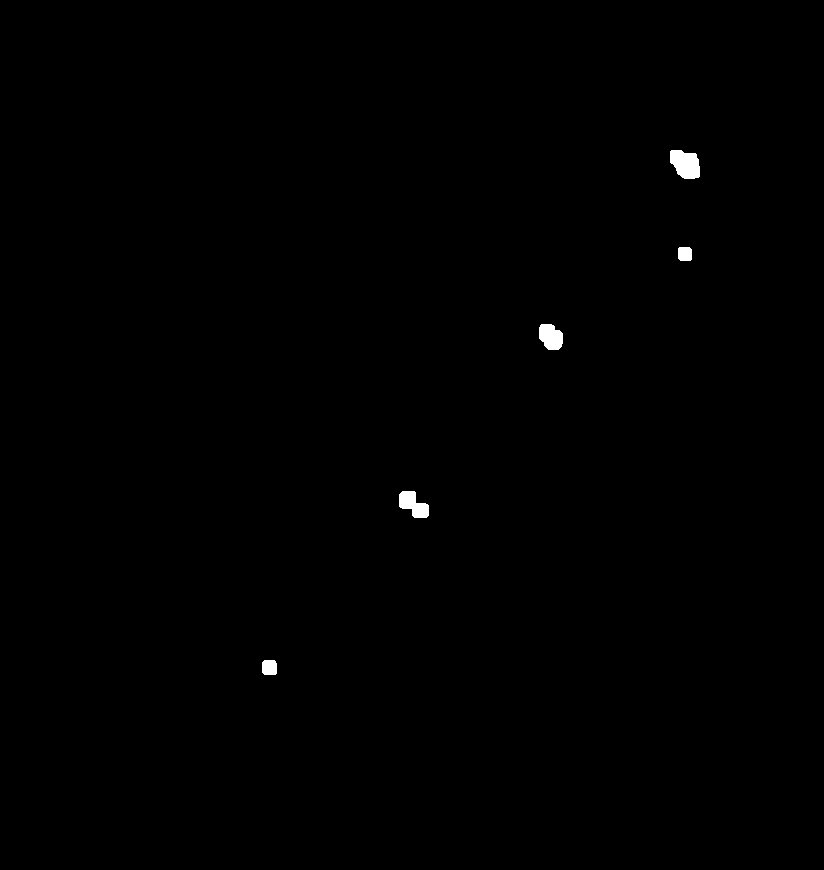
\includegraphics[width=1.0\linewidth]{imagenes/trdQuarterFourierMask.jpg}
			\caption{Tercer cuarto de máscara obtenido a partir de espejar diagonalmente la máscara del segundo cuarto.}
			\label{thirdQuarterMask}
   \end{minipage}\hfill
   \begin {minipage}{0.48\textwidth}
			\centering
			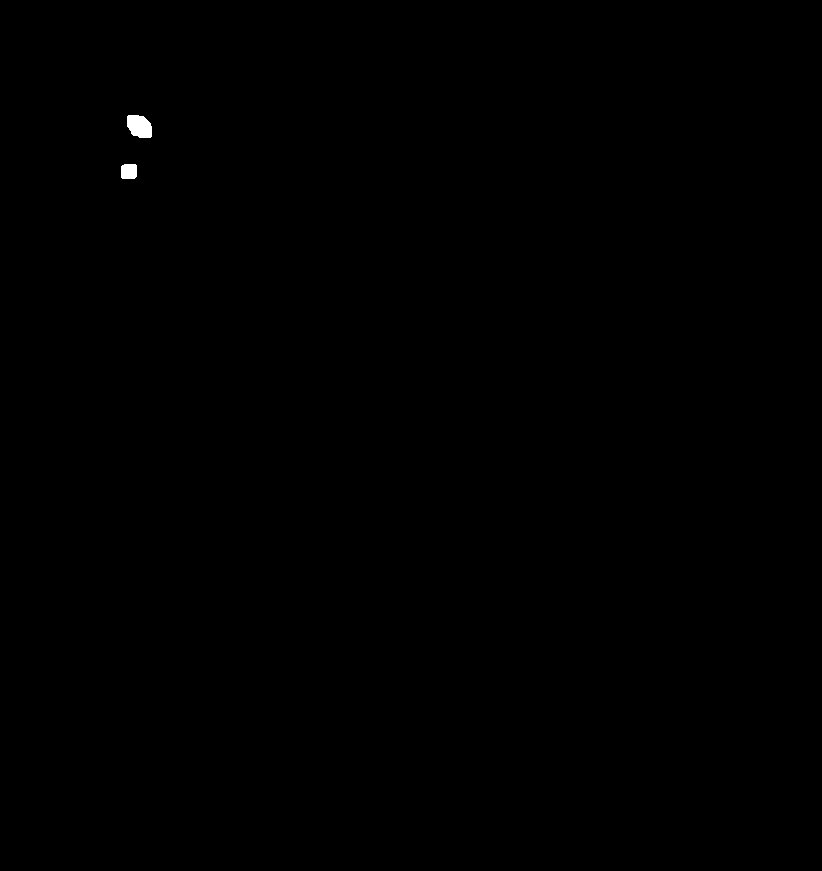
\includegraphics[width=1.0\linewidth]{imagenes/fthQuarterFourierMask.jpg}
			\caption{Cuarto cuarto de máscara obtenido a partir de espejar diagonalmente la máscara del primer cuarto.}
			\label{fourthQuarterMask}
   \end{minipage}
\end{figure}

\textbf{Armado de la imagen con los 4 cuartos:} Una vez obtenidos los 4 cuadrantes, deben ser unidos en una imagen grande, del tamaño de la original. En este caso se debe recordar si tanto filas como columnas eran de cantidad impar. Ya que en ese caso, al armar la imagen de máscara completa se debió completar tal fila o columna faltante al momento de dividir la imagen por la mitad. Se obtiene la imagen que podemos ver en la figura \ref{maskFourierComplete}

\begin{figure}[!htb]
   \centering      
   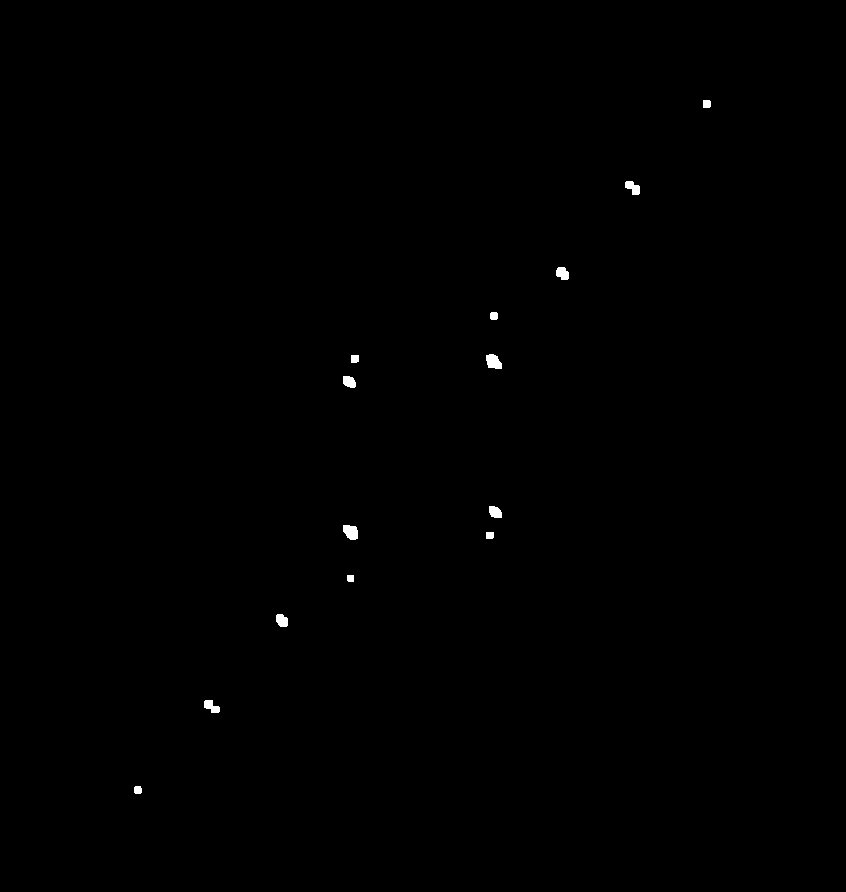
\includegraphics[width=0.5\textwidth]{imagenes/maskFourierComplete.jpg}
 \caption{Máscara de blancos detectados luego de unir los cuatro cuartos.}
 \label{maskFourierComplete}
\end{figure}


\subsubsubsection{Asignar ceros a transformada de Fourier en los píxeles de blancos detectados.}


Una vez que fueron identificados los blancos en la transformada de Fourier que deben ser neutralizados en la imagen, se debe combinar esta información con la de la transformada de Fourier.
Teniendo en cuenta que la máscara disponible tiene valores 1's para los píxeles a neutralizar y 0's para el resto, se necesitará trabajar con el complemento de esta máscara (Figura \ref{maskFourierComplement}). 

\begin{figure}[H]
   \centering      
   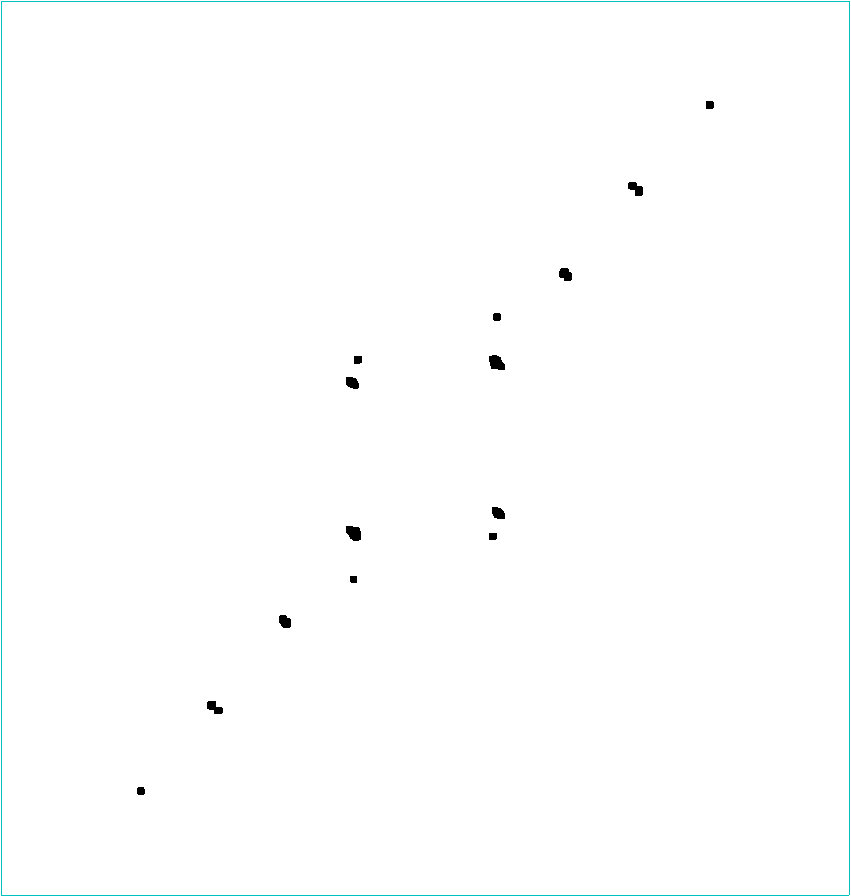
\includegraphics[width=0.5\textwidth]{imagenes/maskFourierComplement.jpg}
 \caption{Complemento de máscara de blancos detectados.}
 \label{maskFourierComplement}
\end{figure}

De esta manera, al aplicar una multiplicación entre la máscara y la imagen de la transformada de Fourier se conservarán todos los valores de la imagen que no son blancos detectados y valores 0 en los blancos detectados. Figura \ref{fourierBlanksCorrected} 

\begin{figure}[H]
   \centering      
   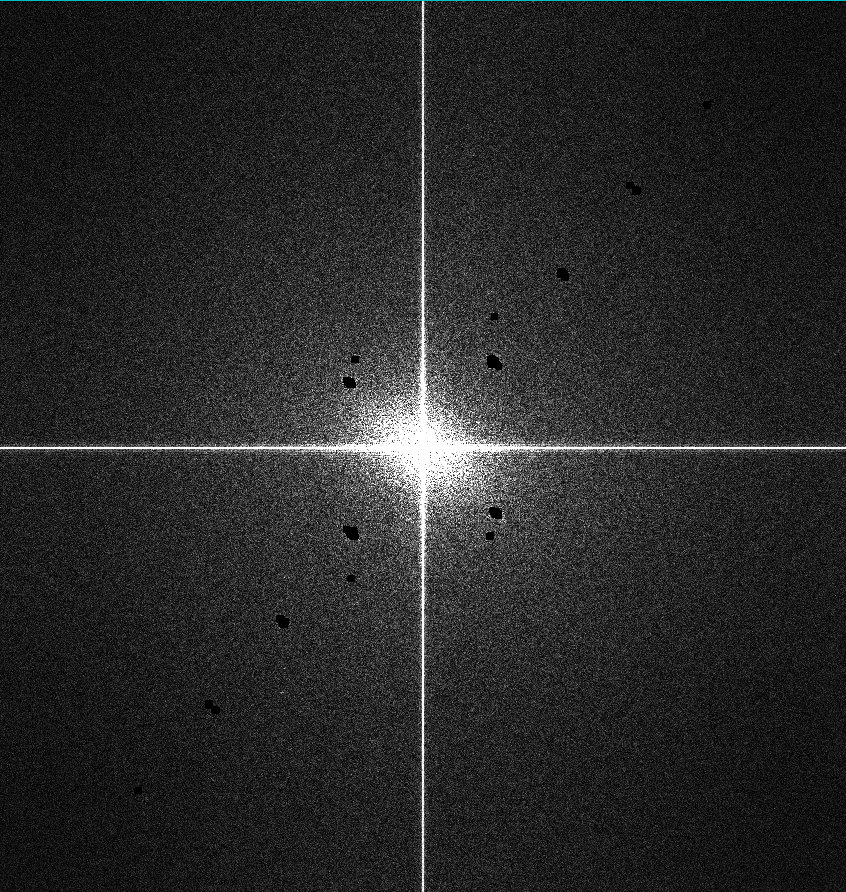
\includegraphics[width=0.5\textwidth]{imagenes/fourierBlanksCorrected.jpg}
 \caption{Imagen de frecuencias de transformada de Fourier con blancos detectados corregidos. Se pueden observas los sectores en negro (valores con cero).}
 \label{fourierBlanksCorrected}
\end{figure}

\subsubsubsection{Retornar las frecuencias cero a su posición original}

Para poder aplicar la antitransformada se debe retornar las frecuencias cero a su posición inicial.

\subsubsubsection{Aplicación de la Antitransformada}



A partir de esta imagen corregida y luego de aplicar la antitransformada a la imagen original, obtendremos que el problema de bandeado fue corregido exitosamente (Figura \ref{SRTMSinFourierCorrected}).

\begin{figure}[H]
   \centering      
   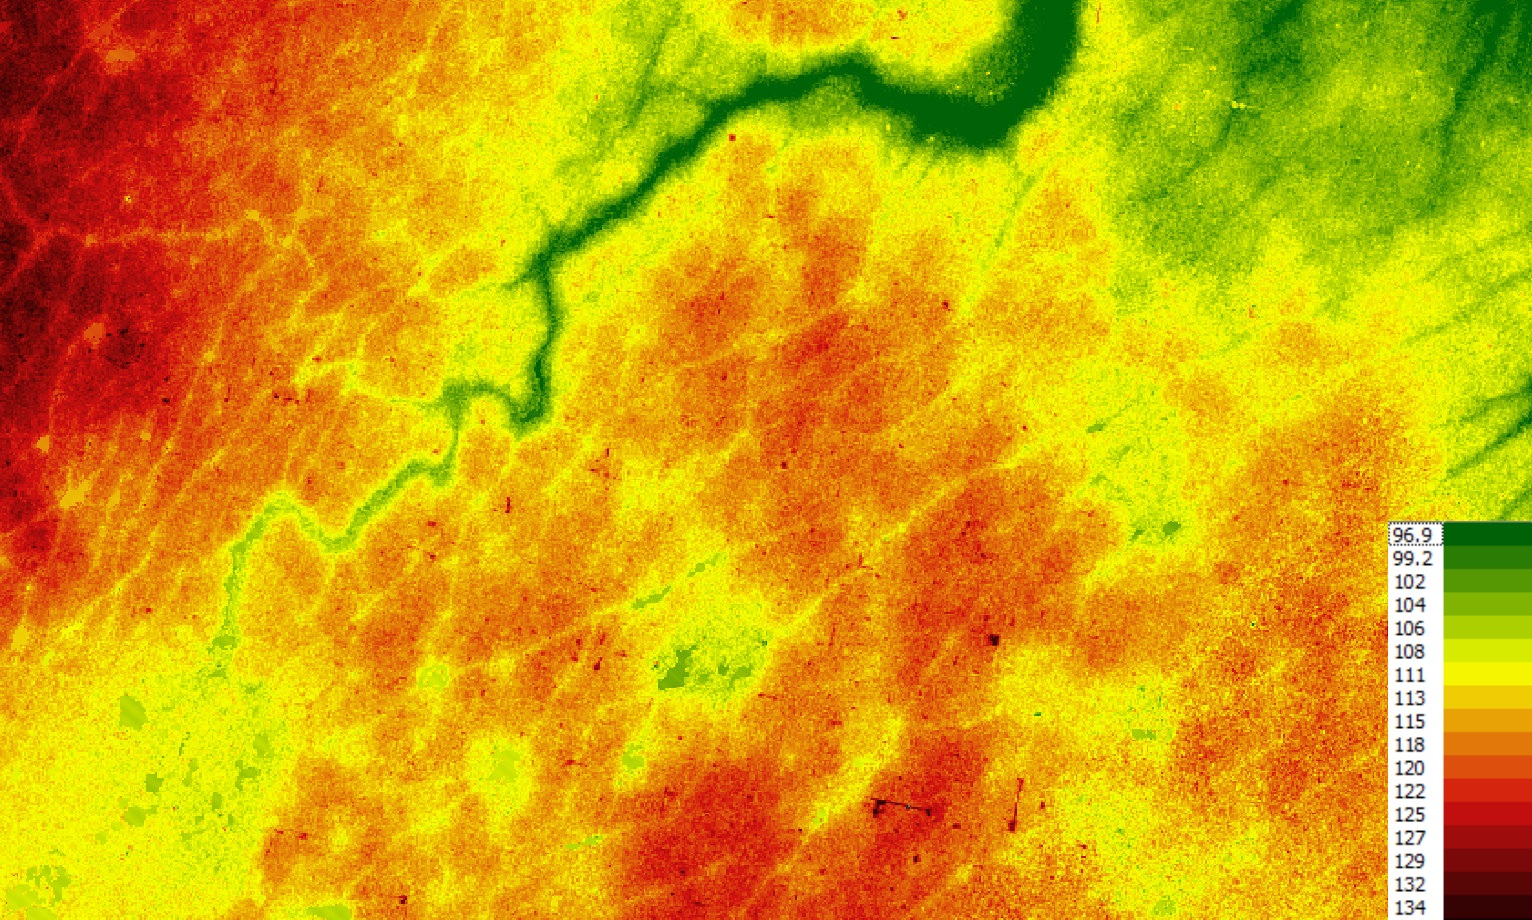
\includegraphics[width=0.85\textwidth]{imagenes/SRTMSinFourierCorrected.jpg}
 \caption{DEM SRTM luego de haber corregido el bandeado utilizando la transformada de Fourier}
 \label{SRTMSinFourierCorrected}
\end{figure}

Comparando esta imagen con la original sin corregir (ver Figura \ref{SinFourier}) podemos distinguir con mayor claridad la ausencia de bandeado.


\subsubsection{Corrección de Cortinas de Árboles}
\label{correccionACortinasDeArboles}

El DEM SRTM presenta la particularidad que en lugares donde existen árboles, registra los valores de altura de estos árboles como si fuera la superficie. Este es un efecto no deseado, dado que para el uso hidrológico que se le pretende dar esto presentaría comportamientos no deseados, ya que el agua debe fluir entre los árboles y no debe representar una barrera como ocurriría en zonas donde no es corregido. Podemos observar como el DEM SRTM original muestra valores más altos en zonas de arboledas (figuras \ref{BingArboledas} y \ref{DEMConArboledas}):

\begin{figure}[!htb]
   \begin{minipage}{0.48\textwidth}
			\centering
			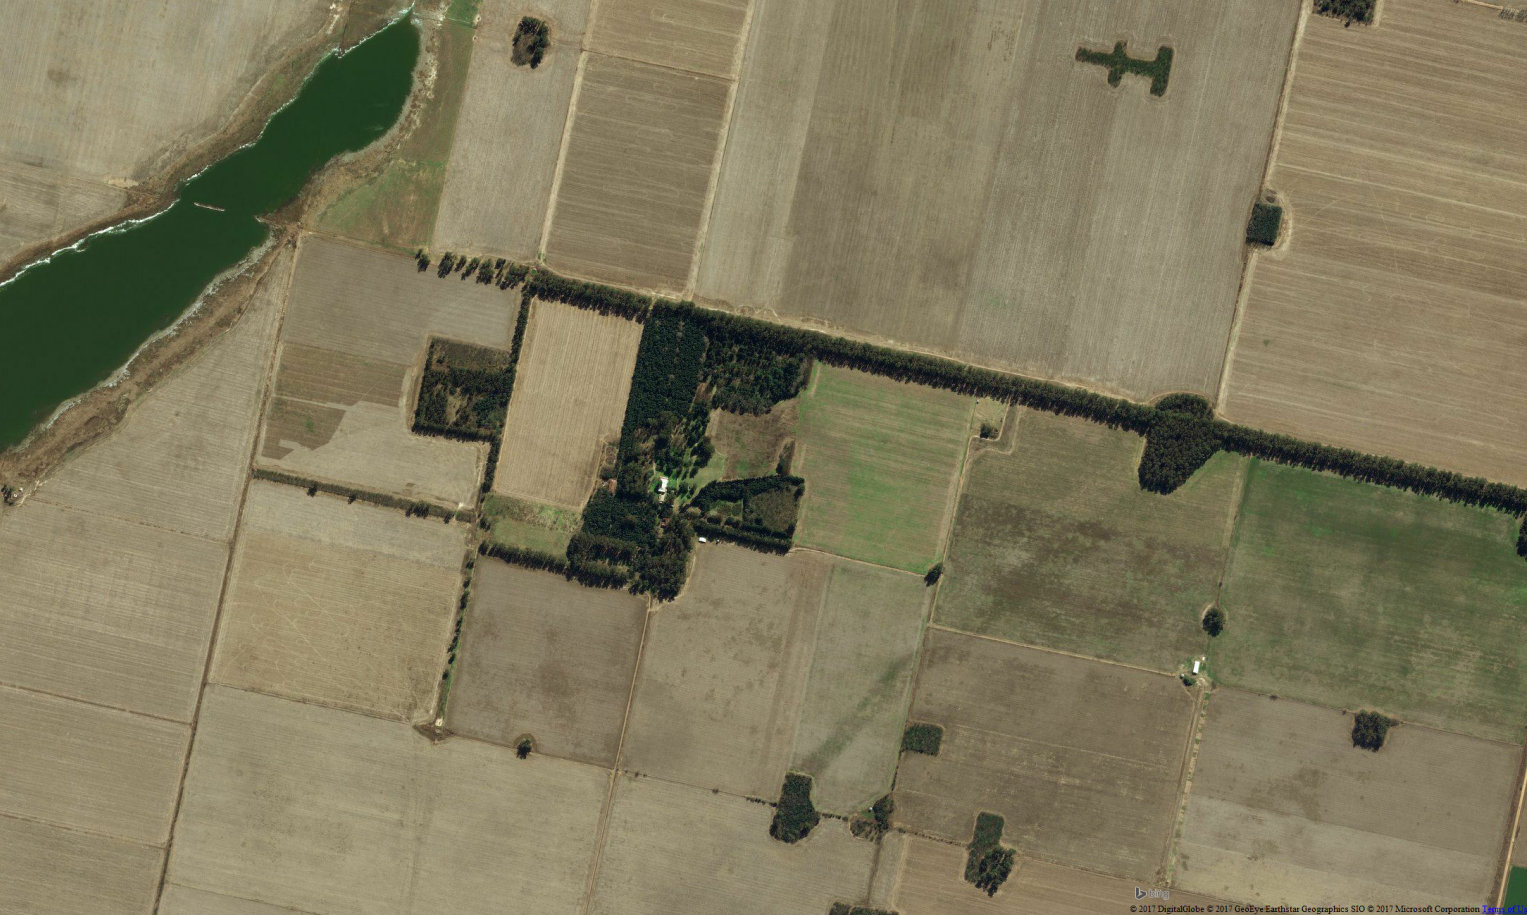
\includegraphics[width=1.0\linewidth]{imagenes/BingArboledas.jpg}
			\caption{Imagen aérea de zona con arboledas.}
			\label{BingArboledas}
   \end{minipage}\hfill
   \begin {minipage}{0.48\textwidth}
			\centering
			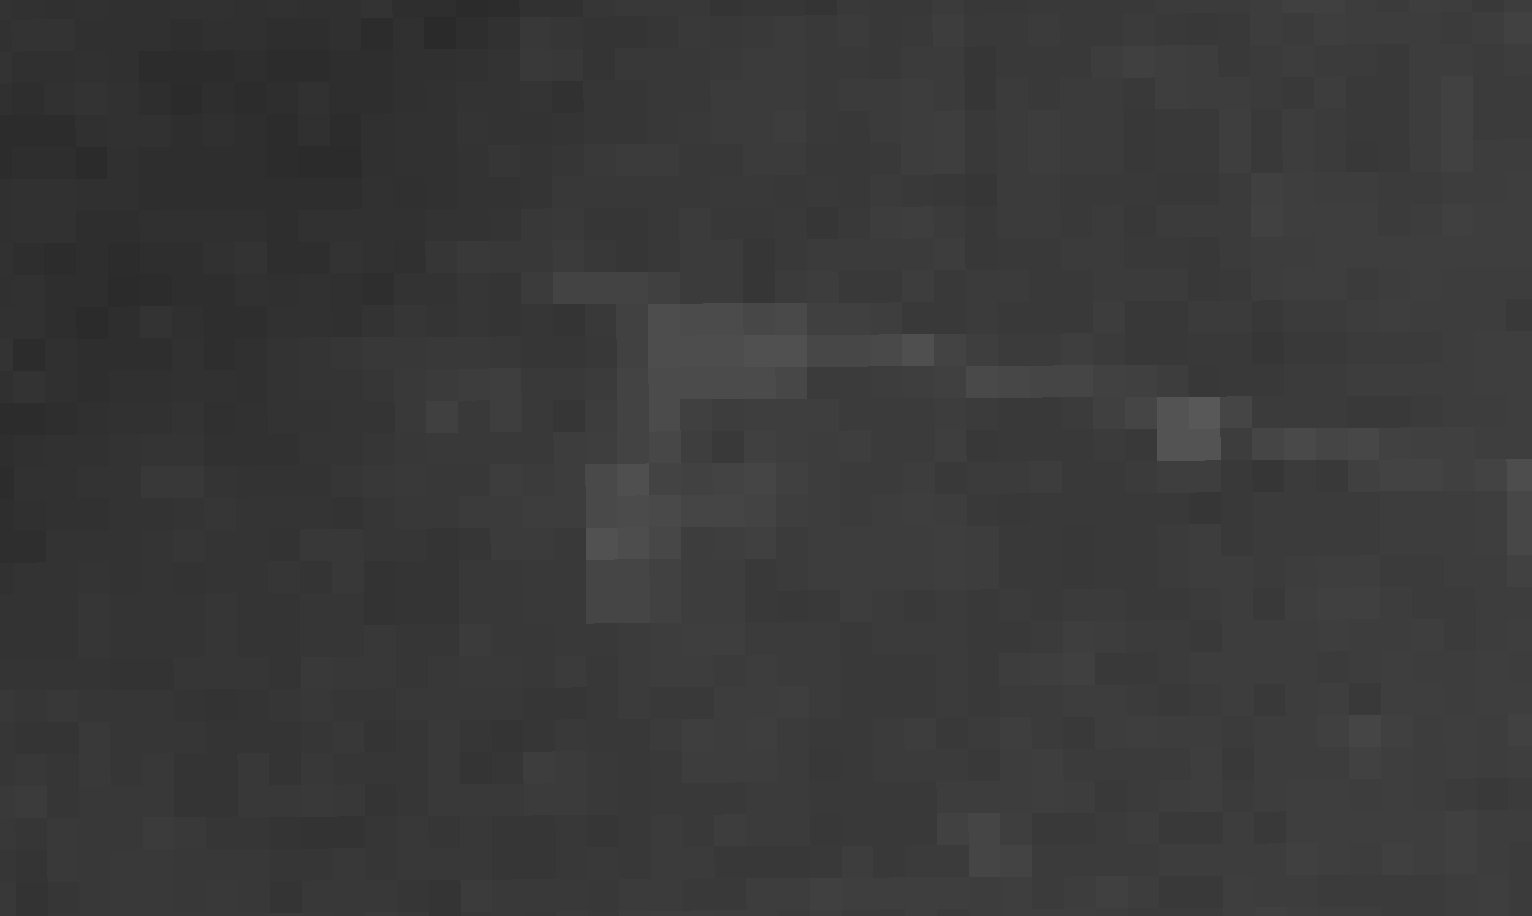
\includegraphics[width=1.0\linewidth]{imagenes/DEMConArboledas.jpg}
			\caption{Área del DEM SRTM que se corresponde con la zona con arboledas}
			\label{DEMConArboledas}
   \end{minipage}
\end{figure}


Es por eso que es necesario poder identificar estos valores no deseados y ajustarlos a los valores reales de altura del suelo. Para poder llevar a cabo esto se debe contar como dato de entrada, ademas del DEM SRTM del área de estudio, una clasificación vegetación obtenida a partir de valores semilla correspondientes a estos conjuntos de árboles.

El DEM SRTM utilizado en este caso es el que ya se encuentra el bandeado corregido por la transformada de Fourier, mencionado en la sección \ref{correccionfourier}.

Una vez que se cuentan con estos datos de entrada se ejecuta una secuencia de pasos que se describen a continuación (Figura \ref{DiagramaArboledas}). 

\begin{figure}[!htb]
   \centering      
   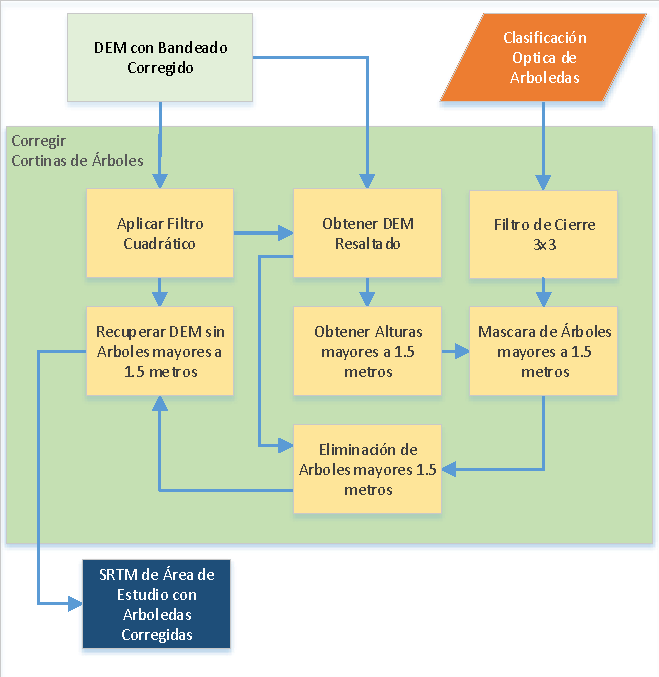
\includegraphics[width=0.55\textwidth]{imagenes/DiagramaArboleda.pdf}
 \caption{Diagrama de flujo de ejecución de pasos para llevar a cabo la corrección de arboledas.}
 \label{DiagramaArboledas}
\end{figure}

Recordemos que esta parte del procesamiento ya se encuentra integrado al programa que procesa completamente el DEM.

\textbf{Aplicación de filtro cuadrático.}

Como primer paso de este proceso se aplica un filtro cuadrático de suavizado de la imagen. El filtro cuadrático que se usa es debido a las características del terreno. Este filtro nos da como resultado un DEM en donde se han planchado todas las irregularidades del terreno y dejando a las ondulaciones más relevantes. A modo de ilustrar el efecto de este filtro sobre el terreno podemos ver la figura \ref{filtroCuadratico}:

\begin{figure}[H]
   \centering      
   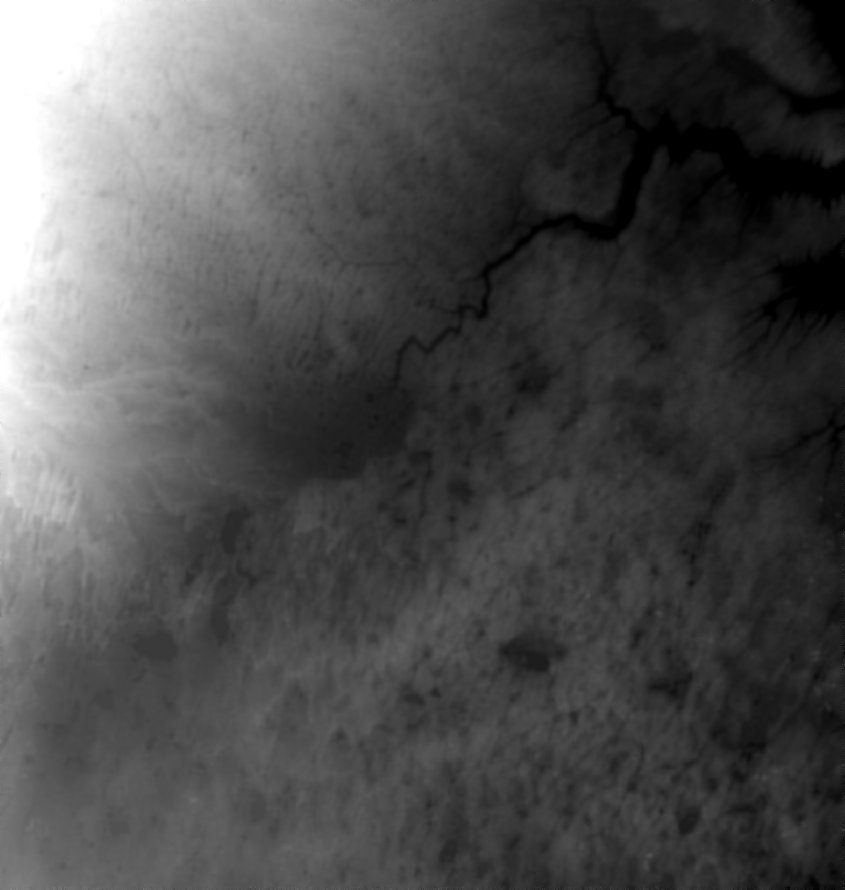
\includegraphics[width=0.5\textwidth]{imagenes/filtroCuadratico.jpg}
 \caption{DEM SRTM luego de haber aplicado el filtro cuadrático}
 \label{filtroCuadratico}
\end{figure}

\textbf{DEM Resaltado}
\label{resta}

A partir de la diferencia entre el DEM SRTM y el suavizado cuadrático obtenido en el paso anterior se puede obtener una imagen que llamaremos "`Resaltado"', Figura \ref{demResaltado}.

\begin{figure}[H]
   \centering      
   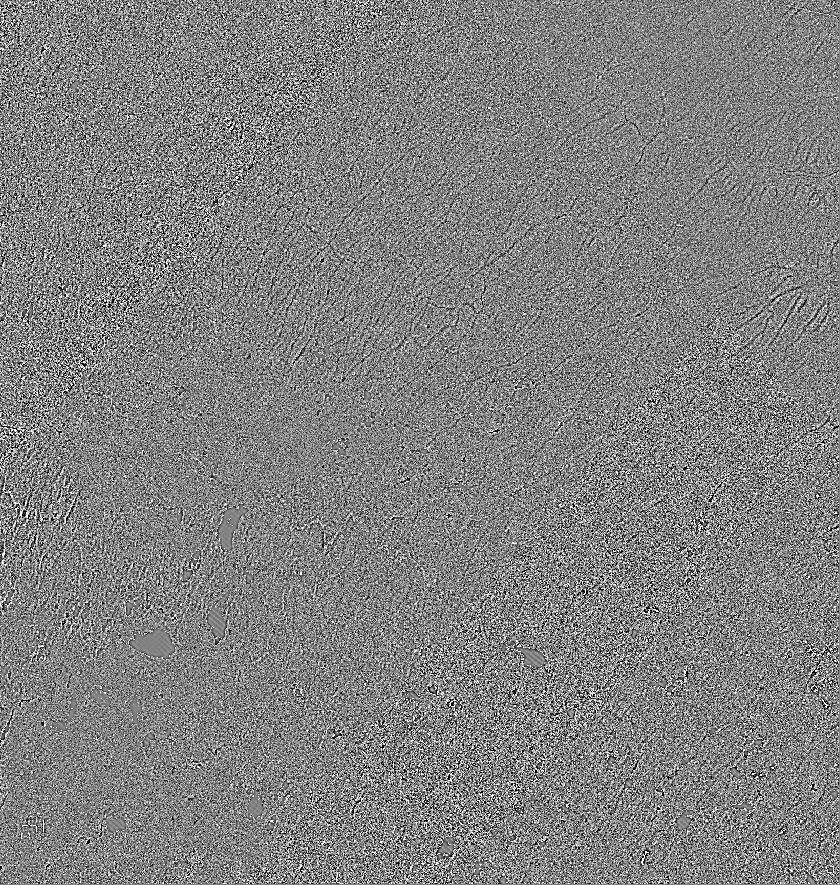
\includegraphics[width=0.5\textwidth]{imagenes/demResaltado.jpg}
 \caption{DEM resaltado, producto de la resta entre el DEM SRTM y el filtro cuadrático.}
 \label{demResaltado}
\end{figure}

Esta imagen representa las alturas que sobresalen abruptamente del suelo.

\textbf{Máscara de valores mayores a 1.5 mts}

Aplicando una condición sobre los valores del DEM Resaltado, podemos obtener una máscara para diferentes alturas, en particular elegimos los valores que superen la altura de 1.5 metros. Figura \ref{maskTrees}

\begin{figure}[H]
   \centering      
   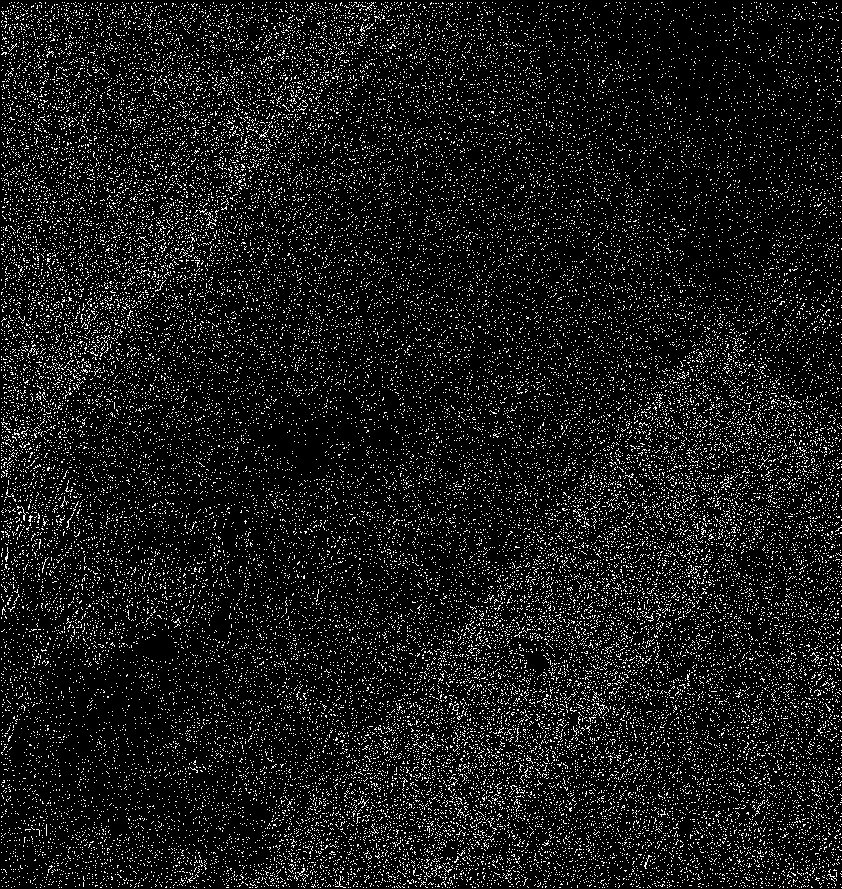
\includegraphics[width=0.5\textwidth]{imagenes/maskTrees.jpg}
 \caption{Máscara de alturas que superan 1.5 metros aplicada al DEM Resaltado.}
 \label{maskTrees}
\end{figure}

\textbf{Máscara de valores mayores a 1.5 mts que son árboles}

Dentro de los valores que superan los 1.5 puede haber alturas que no pertenecen a árboles. Es por eso que es importante poder diferencias las alturas que son árboles o vegetación de las que no lo son. Es acá donde se hace uso de la clasificación de árboles necesaria como dato de entrada, (Sección \ref{clasificacionArboledas}). A esta clasificación se le aplica previamente un filtro de cierre (González \textit{et al.} 1993).
Previamente, se realizó un análisis visual del uso de este filtro evaluando los resultados, se realizaron unas pruebas manuales utilizando un complemento de QGIS y la máscara de arboledas en transparencia, teniendo como fondo la capa de mapas de Bing (Figuras \ref{sinFiltroCierre} y \ref{conFiltroCierre}).

\begin{figure}[H]
   \begin{minipage}{0.48\textwidth}
     \centering
     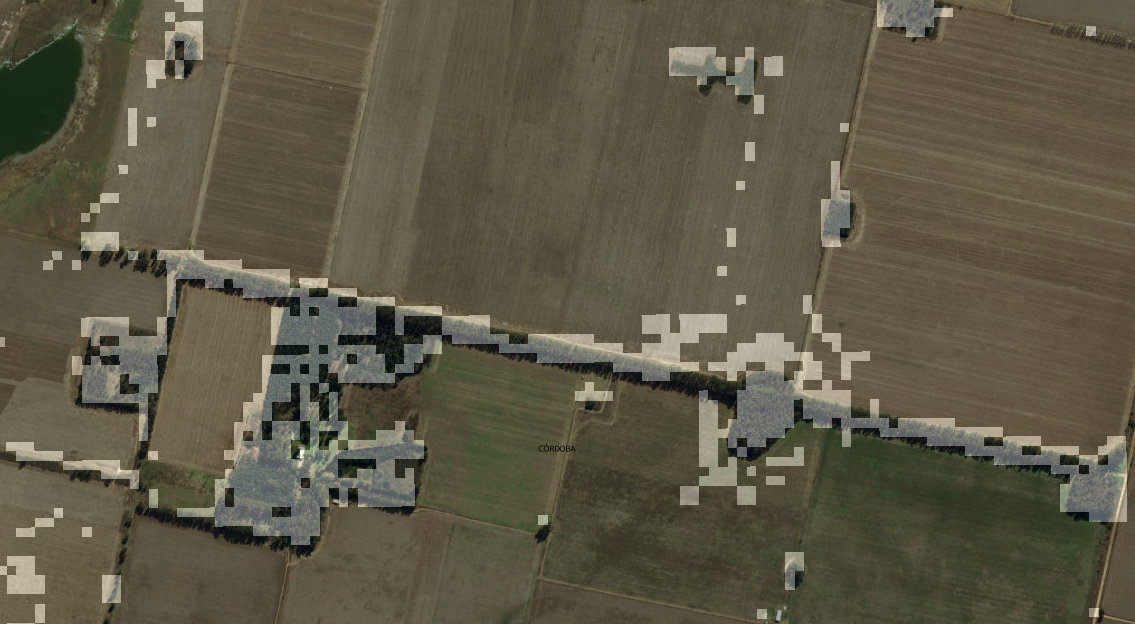
\includegraphics[width=1.0\linewidth]{imagenes/MascaraArbolesSinFiltro}
     \caption{Máscara de arboledas sin filtro de cierre aplicado.}\label{sinFiltroCierre}
   \end{minipage}\hfill
   \begin {minipage}{0.48\textwidth}
     \centering
     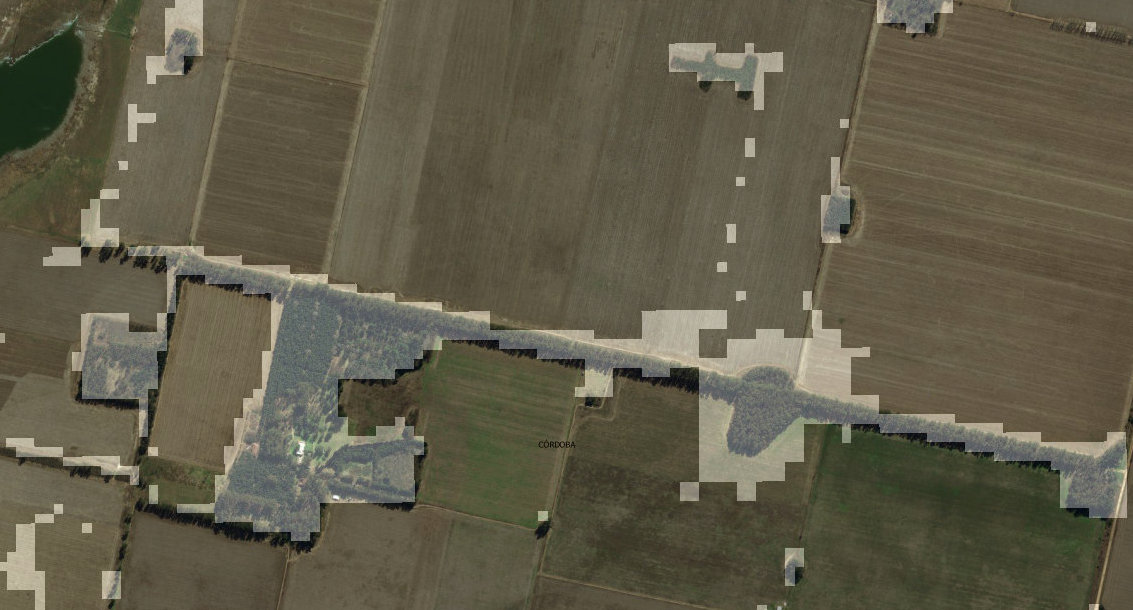
\includegraphics[width=1.0\linewidth]{imagenes/MascaraArbolesConFiltro}
     \caption{Máscara de arboledas con filtro de cierre aplicado.}\label{conFiltroCierre}
   \end{minipage}
\end{figure}

Luego, se necesitan conocer los píxeles que pertenecen a ambas máscaras, alturas mayores a 1.5 mts y arboledas. Esto lo logramos realizando un producto entre ambas imagenes. Teniendo en cuenta que las máscaras tienen valor 1 para valores positivos y 0 en caso negativo de presencia de objeto, la nueva máscara arrojará un valor 1 donde se cumpla la condición en ambas imágenes.

Se obtiene como resultado la siguiente imagen que representa la máscara de árboles mayores a 1.5 metros (Figura \ref{maskTressHeight}).

\begin{figure}[H]
   \centering      
   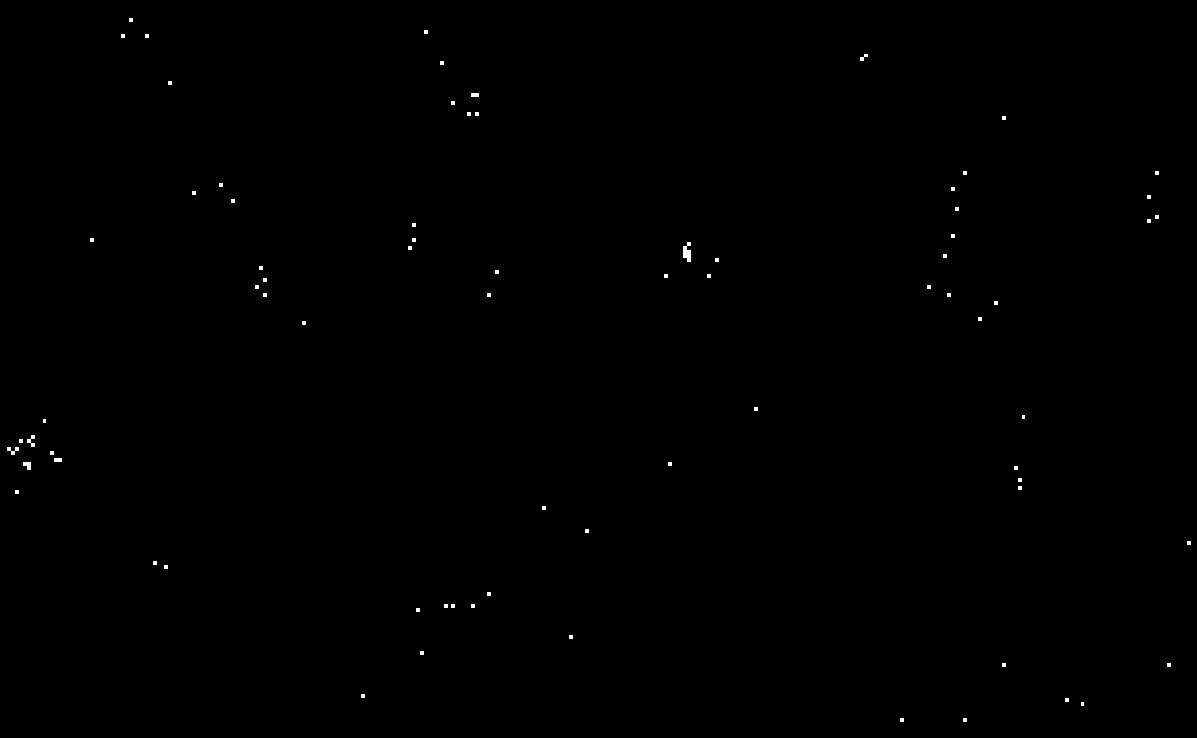
\includegraphics[width=0.95\textwidth]{imagenes/maskTressHeight.jpg}
 \caption{Máscara de alturas que superan 1.5 metros y que son árboles. En puntos blancos se pueden ver los píxeles que cumplen esta condición.}
 \label{maskTressHeight}
\end{figure}

\textbf{Complemento: Máscara de valores menores a 1.5 mts que son árboles}

A partir de la máscara de árboles con valores mayores a 1.5 metros, es posible llevarlos a 0, estas alturas son consideradas no deseadas. Una técnica para esto es obtener el complemento de la máscara de árboles. Esto se logra restarle la máscara de árboles a una imagen completamente compuesta por unos. De esta manera en la nueva máscara, donde había un 1 habrá un 0 y donde había un 0 ahora habrá un 1 (Figura \ref{maskTressHeightCompl}).


\begin{figure}[H]
   \centering      
   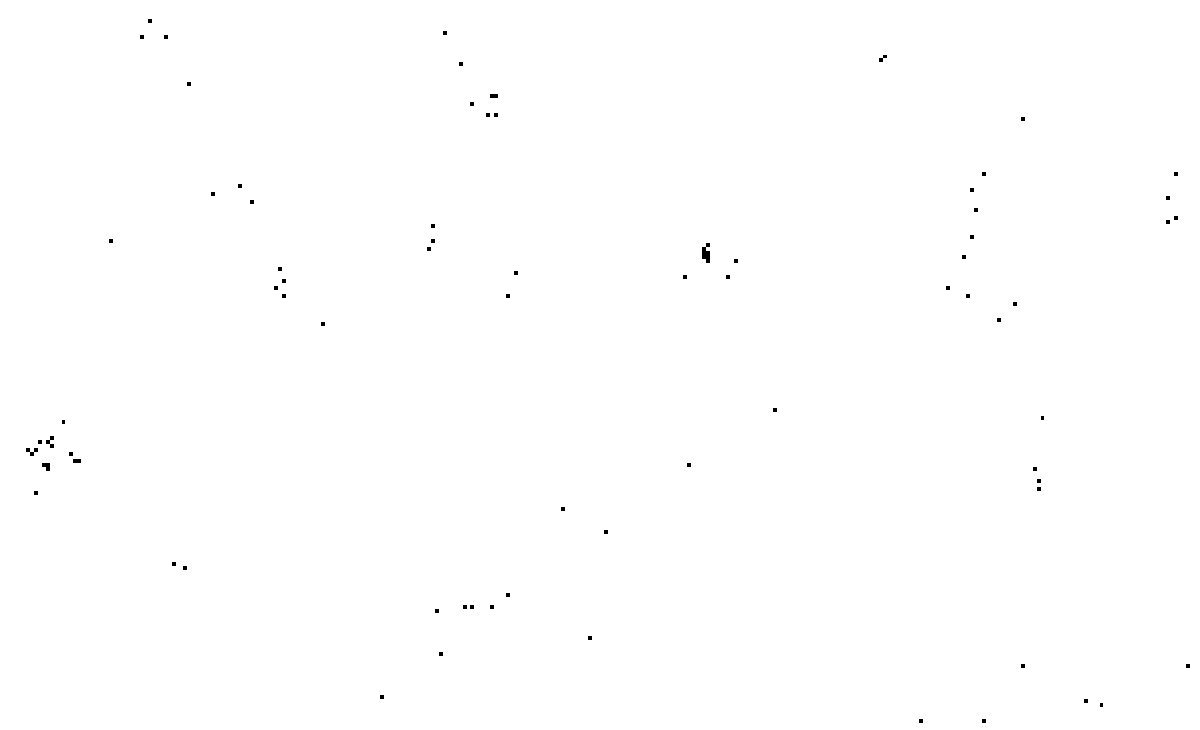
\includegraphics[width=0.85\textwidth]{imagenes/maskTressHeightCompl.jpg}
 \caption{Complemento de máscara de alturas que superan 1.5 metros y que son árboles. En este caso en puntos negros se pueden ver los píxeles que cumplen esta condición.}
 \label{maskTressHeightCompl}
\end{figure}


\textbf{DEM Resaltado sin árboles}

A partir del producto entre el complemento de la máscara de árboles y el DEM Resaltado se obtiene una imagen de alturas resaltadas, sin árboles mayores a 1.5 metros. Esto se debe a que en los lugares donde hay árboles mayores a 1.5 la máscara contiene un valor 0 y en el resto un valor 1. El producto deja todo como está, excepto en los lugares con árboles, donde el valor es llevado a 0. Es difícil distinguir a simple vista donde fueron corregidos estos valores. 

%\begin{figure}[!htb]
   %\centering      
   %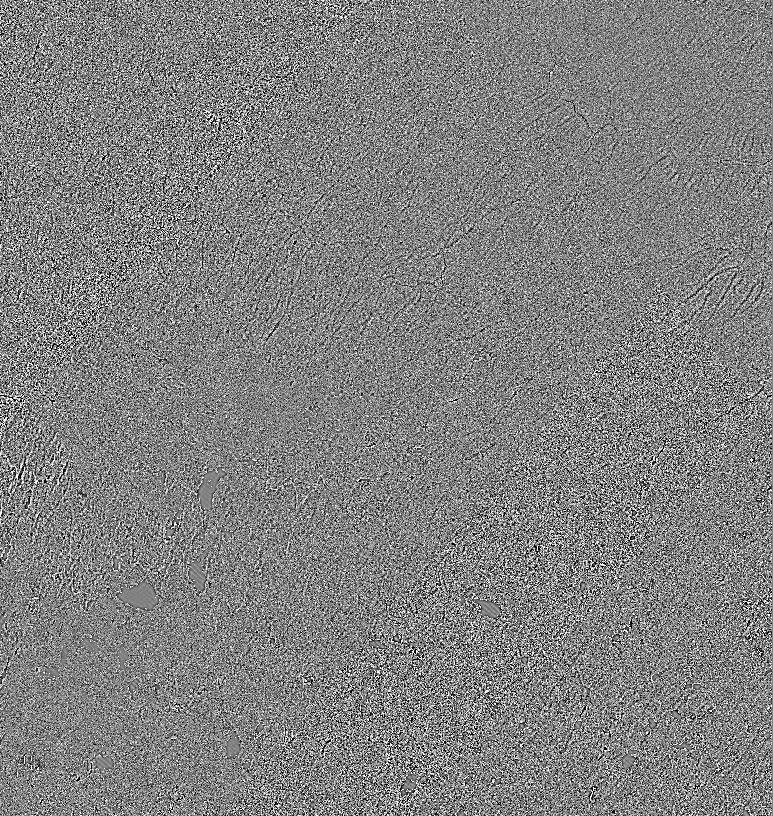
\includegraphics[width=0.7\textwidth]{imagenes/demResaltadoSinArboles.jpg}
 %\caption{DEM Resaltado en donde fueron corregidas los árboles detectados. Es difícil apreciar a simple vista donde fueron corregidos estos valores.}
 %\label{demResaltadoSinArboles}
%\end{figure}

\textbf{SRTM corregido: sin árboles}

Una vez eliminados los árboles de la imagen de alturas resaltadas, se puede reconstruir el DEM SRTM que contiene estas correcciones. Esto se puede llevar a cabo aplicando el proceso inverso al paso \ref{resta}, es decir sumando el DEM Resaltado (ya corregido en el paso anterior) más el DEM Suavizado por el filtro cuadrático.

Se obtiene de esta manera, el DEM SRTM con corrección de cortinas de árboles (Figura \ref{fig:comparacionArboledas}):

\begin{figure}[H]
	\centering
	\subfigure[DEM SRTM sin arboledas corregidas]{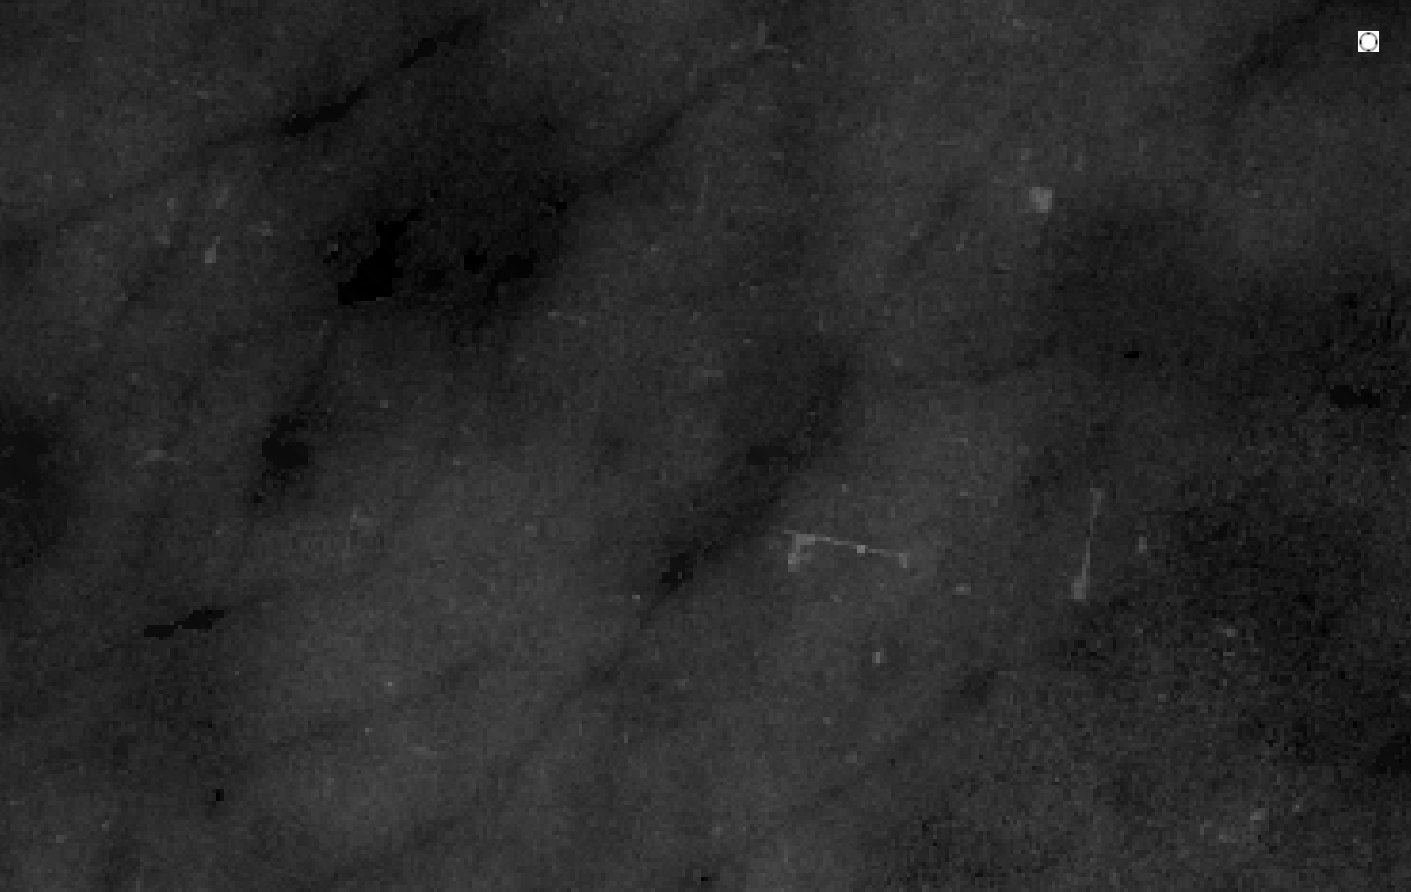
\includegraphics[width=0.49\linewidth]{imagenes/ArboledasNoCorregidasDEM}}
	\subfigure[DEM SRTM con arboledas corregidas]{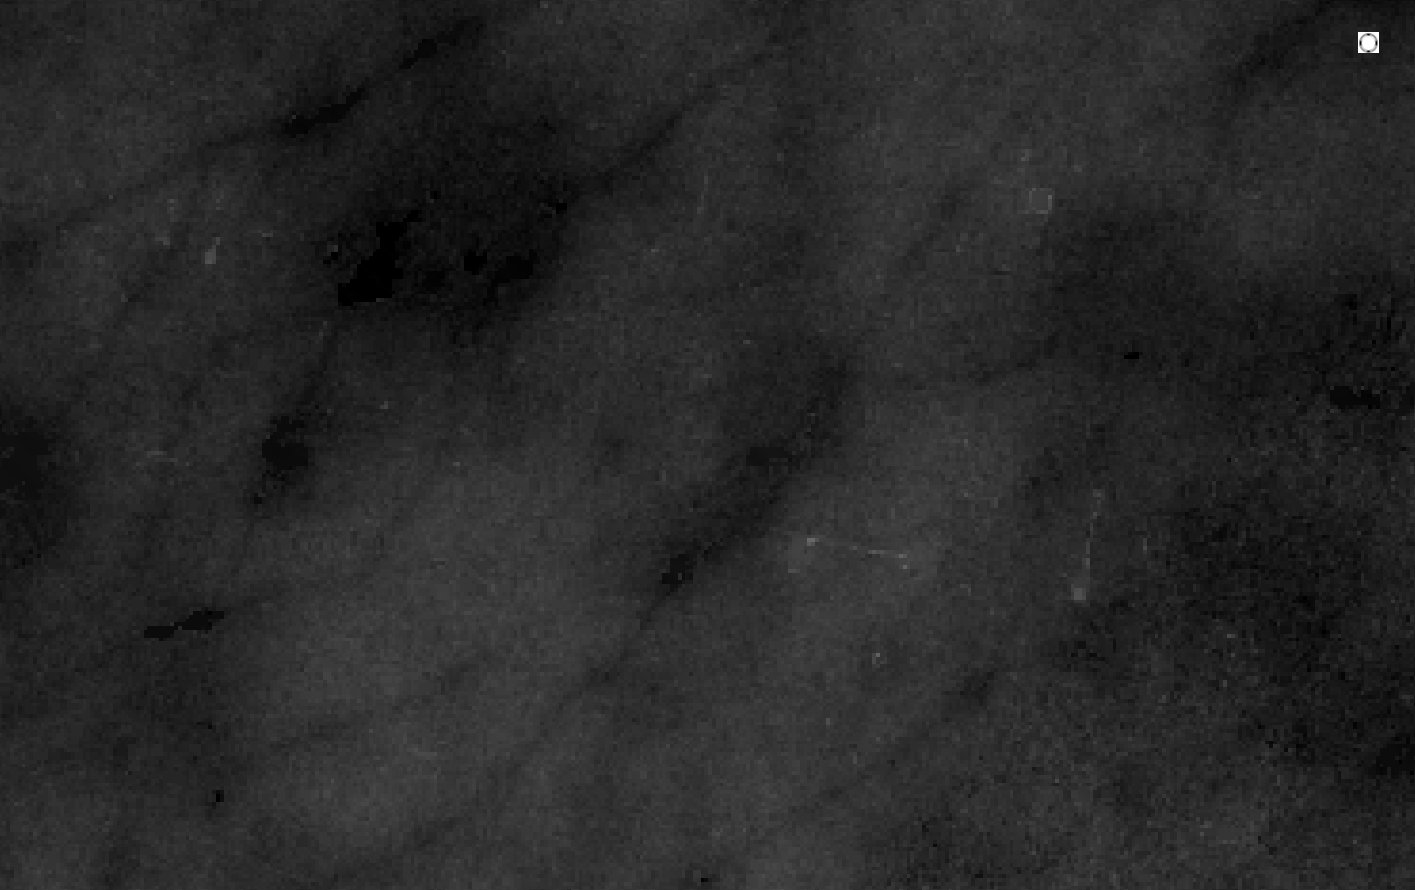
\includegraphics[width=0.49\linewidth]{imagenes/ArboledasCorregidasDEM}}
	\caption{Comparación de una parte del área de estudio donde se puede observar la corrección de arboledas}
	\label{fig:comparacionArboledas}
\end{figure}

\textbf{Observación sobre la corrección de arboledas.}
\label{obscorreccionArboledas}

Durante el procesamiento se observó que en determinados casos la presencia de arboledas no era corregida de la manera esperada. Analizando visualmente algunos casos se determinó que se debe tener en cuenta que el DEM SRTM fue desarrollado a partir de imágenes de radar tomadas en el año 2000.

Para realizar la corrección de arboledas se utilizaron imágenes Landsat 8 del año 2017 que ya proveen algunas correcciones que simplifican el procesamiento. Esta diferencia en tiempo puede provocar que algunas arboledas no sean corregidas por variaciones en la presencia de árboles desde el año 2000 al año 2017. Esto puede ser observado en la siguiente figura \ref{fig:observacionArboledas}:

\begin{figure}[H]
	\centering
	\subfigure[DEM SRTM con presencia de arboledas]{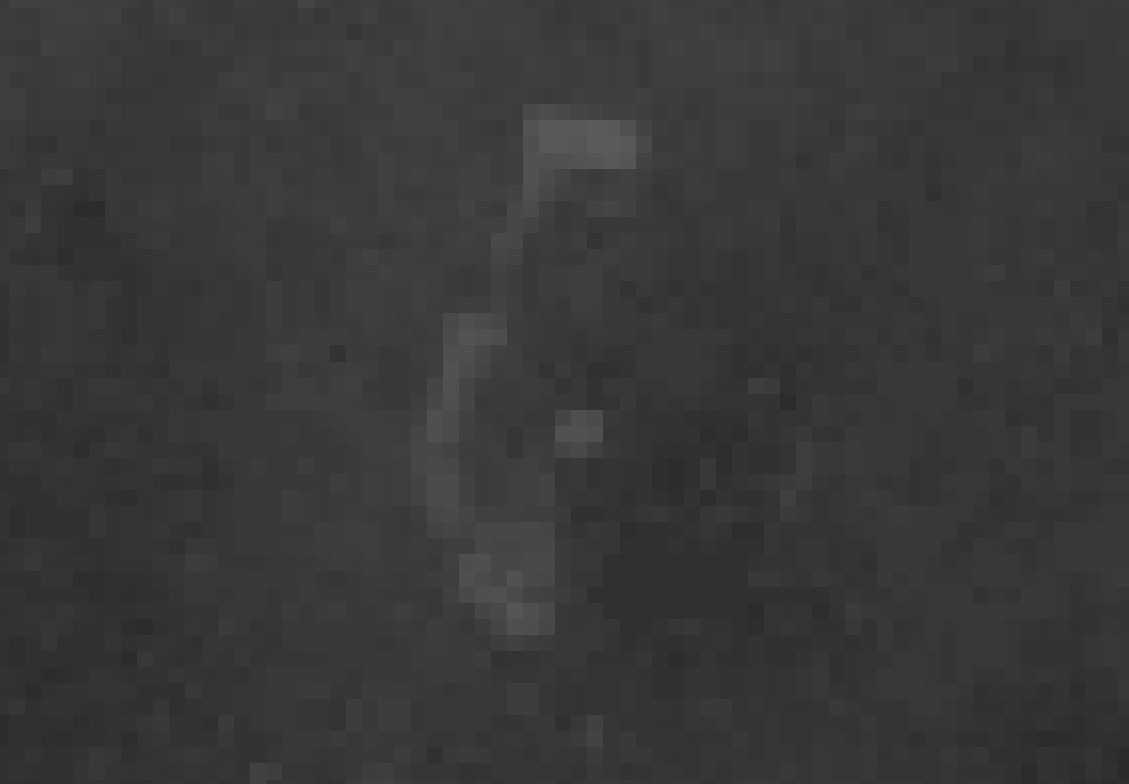
\includegraphics[width=0.49\linewidth]{imagenes/ObservacionDEM}}
	\subfigure[Imagen Bing actual dónde se ve presencia de árboles sólo en una parte]{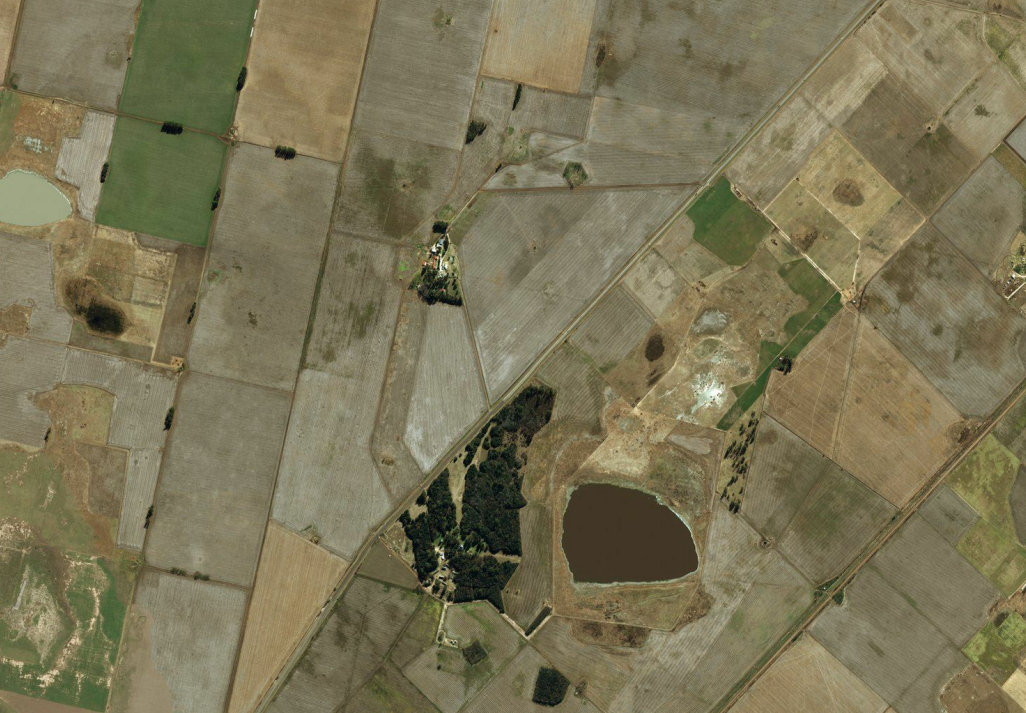
\includegraphics[width=0.49\linewidth]{imagenes/ObservacionBing}}
	\caption{Correspondencia de DEM SRTM con imagen actual de Bing. Se esperaría que en los píxeles más claros existan arboledas, los cuales deberían ser capturados por la clasificación de arboledas.} \label{fig:observacionArboledas}
\end{figure}


\subsection{Procesamiento a HydroSHEDS para extracción de lagunas, ríos y cañadas}
%%%%%%%%%%%%%%%%%%%%%%%%%%%%%%%%%%%%%%%%%%%%%%%%%%%%%%%%%%%%%%%%%%%%%%%%%%%%%%%%%%

El DEM de HydroSHEDS ofrece interesantes características para uso hidrológico ya que provee una mejor definición de las cañadas y de pequeñas lagunas del terreno. Asimismo, viene con la desventaja del bandeado inherente al DEM, excepto en los cuerpos de agua que provee. La existencia de estos cuerpos de agua en donde no existe el bandeado dificulta la corrección por transformada de Fourier debido a que cuando se intenta corregir introduce errores en estos cuerpos de agua, como vimos en la sección \ref{aplicacionBandeado}. Debido a esto, solo se extraen los datos correspondientes a lagunas, ríos y cañadas.

Las operaciones realizadas a partir de HydroSHEDS son descriptas a continuación (Figura \ref{DiagramaLagunas}):

\begin{figure}[H]
   \centering      
   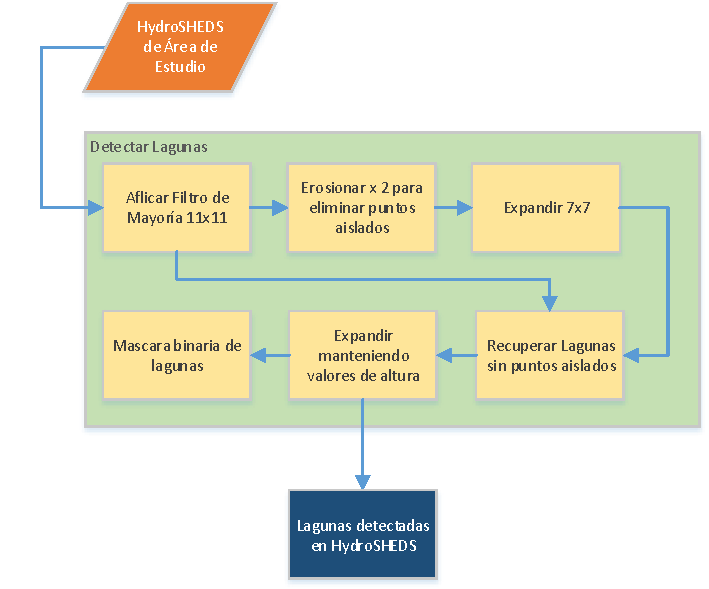
\includegraphics[width=0.65\textwidth]{imagenes/DiagramaLagunas.pdf}
 \caption{DEM Resaltado en donde fueron corregidas los árboles detectados. Es difícil apreciar a simple vista donde fueron corregidos estos valores.}
 \label{DiagramaLagunas}
\end{figure}

\subsubsection{Conversión de formato adf a tif (HydroSHEDS)}

En primer lugar el archivo HydroSHEDS viene en formato adf, se debe convertir a formato tif para poder manipularlo de igual manera que el resto de los datos. Para esto se utiliza una herramienta provista por python GDAL: $gdal\_translate.exe$
Para poder realizar de manera correcta la conversión se debe pasar como argumento el nombre de archivo .adf que debe estar ubicado junto con el resto de los archivos provistos por el sitio USGS.

\subsubsection{Detección de Lagunas}
\label{deteccionLagunas}

 Considerando que una de las ventajas que ofrece HydroSHEDS es la definición de cavidades de probables lagunas en el terreno, es importante rescatar esta característica de este producto y que se encuentre presente en el DEM procesado final.

\textbf{Filtro de Mayoría}

Para eso se definió un filtro de Mayoría con una ventana de 11 x 11, el cual decide si el píxel central pertenece a una laguna si la mayoría de sus vecinos dentro de la ventana de 11 x 11 tienen el mismo valor. En caso de ser así, el píxel del núcleo conserva su valor original, (el que trae del DEM HydroSHEDS). Caso contrario, toma el valor 0. Figura \ref{filtroMayoria}

\begin{figure}[H]
   \centering      
   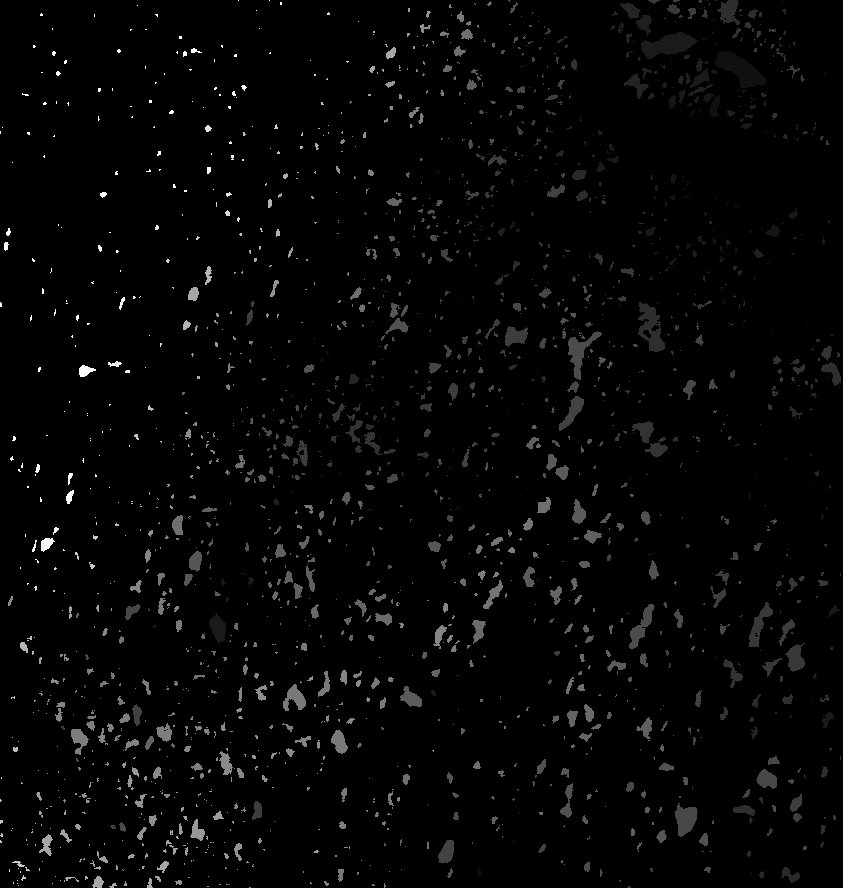
\includegraphics[width=0.5\textwidth]{imagenes/filtroMayoria.jpg}
 \caption{Lagunas detectadas aplicando filtro de mayoría. Se pueden ver las lagunas en escala de grises}
 \label{filtroMayoria}
\end{figure}

\textbf{Eliminación de píxeles aislados}

Luego de la máscara obtenida en el paso anterior, se observo la presencia de numerosos píxeles aislados, o agrupados solo en conjuntos de dos o tres píxeles. Estos valores no son deseados, ya que no representan algún cuerpo de agua, es solo un caso aislado, es por eso que no deben formar parte de las lagunas a detectar. Para la eliminación de estos casos se procedió de la siguiente manera:
		
		\textbf{Erosión:} Se aplicó un filtro de erosión con 2 iteraciones a la máscara obtenida en el paso anterior. Esto desgasta los bordes de las lagunas sometidas a la erosión. Varias lagunas reducirán su tamaño y las más pequeñas o píxeles aislados desaparecerán. Figura \ref{puntosAislados}
		
\begin{figure}[H]
   \centering      
   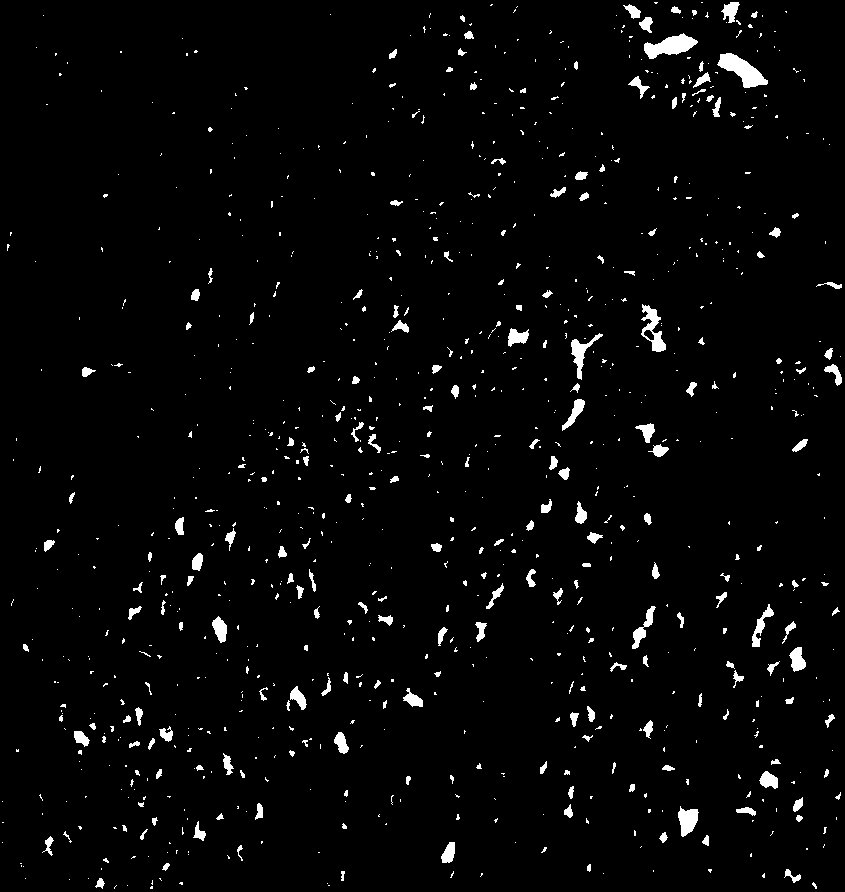
\includegraphics[width=0.5\textwidth]{imagenes/puntosAislados.jpg}
 \caption{Luego del filtro de erosión se eliminan puntos aislados.}
 \label{puntosAislados}
\end{figure}		

		\textbf{Expansión:} Luego de la erosión, se aplica un filtro de expansión, con el objetivo de recuperar las lagunas originales. Se expandirán los píxeles pertenecientes a la máscara de lagunas, muchos píxeles aislados desaparecieron en el paso anterior y no producirán nada para expandir. Figura \ref{lagunasExpandidas}
		
\begin{figure}[H]
   \centering      
   \includegraphics[width=0.5\textwidth]{imagenes/lagunasExpandidas.jpg}
 \caption{Las lagunas fueron expandidas con una ventana de 7x7.}
 \label{lagunasExpandidas}
\end{figure}
		
		\textbf{Producto:} Con la expansión realizada, se amplió el margen de las lagunas detectadas, pero de manera abrupta. Es por eso que para la recuperación final de lagunas se aplica un producto entre la detección original de lagunas y la última máscara expandida, esto nos devuelve la máscara de píxeles que pertenecen a ambas máscaras, provocando:
		
		\begin{itemize}
			\item Desaparición de píxeles sueltos o pequeños grupos de píxeles.
			\item Conservación de demarcación de lagunas originalmente detectadas.
		\end{itemize}		
		
		Podemos ver el resultado en la figura \ref{lagunasDetectadas}

\begin{figure}[H]
   \centering      
   \includegraphics[width=0.5\textwidth]{imagenes/lagunasDetectadas.jpg}
 \caption{Lagunas obtenidas luego de eliminación de puntos aislados.}
 \label{lagunasDetectadas}
\end{figure}		
		
\textbf{Expansión de lagunas detectadas}

Las lagunas detectadas tienen bordes muy definidos, una expansión a esta detección de lagunas puede lograr abarcar un poco más del borde la laguna, lo que lograría una poco más de uniformidad sobre el cuerpo de agua (Figura \ref{dilationLagoons}).

\begin{figure}[H]
   \centering      
   \includegraphics[width=0.5\textwidth]{imagenes/dilationLagoons.jpg}
 \caption{Lagunas expandidas.}
 \label{dilationLagoons}
\end{figure}		


\subsubsection{Procesamiento de Ríos y Cañadas.}

Como vimos en la sección \ref{vectorRiosArea} uno de los datos de entrada es un archivo vectorial de ríos y cañadas del área que cubre abarca completamente el área de estudio. En la figura \ref{caniada} podemos observar una foto de un ejemplo real de una cañada en zona de llanuras:

\begin{figure}[H]
   \centering      
   \includegraphics[width=0.85\textwidth]{imagenes/caniada.jpg}
 \caption{Cañada en llanura correspondiente a la zona de Corral de Bustos (sur-este de la provincia de Córdoba)}
 \label{caniada}
\end{figure}

El objetivo del uso de este dato de entrada es poder determinar los ríos y cañadas relevantes para poder extraer esta información del DEM HydroSHEDS. Para esto, a este dato de entrada se le tuvo que realizar una serie de procesamientos descriptos en el siguiente diagrama (Figura \ref{DiagramaRios}):

\begin{figure}[H]
   \centering      
   \includegraphics[width=0.85\textwidth]{imagenes/DiagramaRios.pdf}
 \caption{Diagrama de flujo del procesamiento de ríos y cañadas a partir de los datos de entrada.}
 \label{DiagramaRios}
\end{figure}	


\textbf{Rasterizar Vector de Ríos}

Como primer paso se procedió a rasterizar el archivo vectorial. Esto significa convertir a imagen de píxeles los datos vectoriales según los valores de cada línea y dejando en cero donde no existen vectores. Esto se realizó con una herramienta de la librería $gdal$ llamada $gdal_rasterize$ indicando filas y columnas del raster de destino.

%Como resultado se obtiene la siguiente imagen. Figura \ref{RiosRasterizados}

%\begin{figure}[H]
   %\centering      
   %\includegraphics[width=0.85\textwidth]{imagenes/RiosRasterizados.jpg}
 %\caption{Raster de ríos y cañadas. No se aprecian todos los ríos y cañadas debido a la escala de grises y al zoom de la imagen.}
 %\label{RiosRasterizados}
%\end{figure}

\textbf{Crear Máscara de Ríos}

El raster de ríos y cañadas generados posee los valores que traen los vectores, se necesita tener una máscara binaria de ríos, por lo que se crea la misma a partir de una condición sobre los píxeles de la imagen de ríos. %Figura \ref{MascaraRios}

%\begin{figure}[H]
   %\centering      
   %\includegraphics[width=0.85\textwidth]{imagenes/MascaraRios.jpg}
 %\caption{Máscara de ríos y cañadas. Muchos de los ríos y cañadas se los ve interrumpidos pero se debe al zoom de la imagen y al ancho de las líneas que denotan los ríos y cañadas}
 %\label{MascaraRios}
%\end{figure}

\textbf{Expandir máscara de Ríos}

Teniendo en cuenta que el archivo vectorial ofrece los ríos y cañadas como vectores, estos se ven como líneas delgadas en la superficie. Tales ríos y cañadas en la realidad representan una superficie más amplia que la línea por la cual son representados, es por eso que se aplica un filtro de dilatación a la máscara obtenida en el paso anterior. Figura \ref{riosExpandidos}

\begin{figure}[H]
   \centering      
   \includegraphics[width=0.5\textwidth]{imagenes/riosExpandidos.jpg}
 \caption{Máscara de ríos y cañadas expandida con filtro de dilatación de 3x3. En esta imagen se pueden apreciar mejor todos los ríos y cañadas debido a que se ensancharon los mismos por el filtro aplicado.}
 \label{riosExpandidos}
\end{figure}

\textbf{Enrutar Ríos}

En algunos casos, la representación vectorial de los ríos y cañadas por parte del dato de entrada no sigue exactamente el trayecto de los mismos, y esto se puede ver superponiendo ambas capas. Figura \ref{riverToEnroute}

\begin{figure}[H]
   \centering      
   \includegraphics[width=0.85\textwidth]{imagenes/riverToEnroute.jpg}
 \caption{Se puede observar como el vector de ríos ya rasterizado (amarillo) no sigue en todos lados el río o cañada de HydroSHEDS (negro).}
 \label{riverToEnroute}
\end{figure}

Para esto se aplicaron varios procesos, entre ellos la creación e implementación de un filtro que se encargue de "`enrutar"' adecuadamente los ríos y cañadas de acuerdo como están en el DEM HydroSHEDS. 

\textbf{Filtro de Enrutamiento de Ríos y Cañadas:} 

Se desarrolló un filtro para la detección de canales, ríos y cañadas el cual se denominó: $enrouteRivers$. El funcionamiento del filtro se describe a continuación:

\begin{itemize}
	\item Este filtro consta de una ventana de 5x5. 
	\item A diferencia de la mayoría de los filtros que se usan en imágenes los cuales son aplicados al total de la imagen, en este caso es sólo aplicado a los píxeles con valor 1, es decir a los píxeles que indican presencia de río o cañada. 
	\item Estos índices de la imagen a los cuales serán aplicados son tomados de la imagen de máscara que se tiene hasta el momento y la imagen evaluada es el DEM de HydroSHEDS.
	\item A partir de estas dos imágenes combinadas por el filtro se obtendrá una tercera imagen.
	\item Esta tercera imagen contendrá una nueva máscara de ríos y cañadas en donde los valores serán establecidos en 1 siguiendo el siguiente algoritmo:	
	\begin{itemize}
		\item La ventana se posiciona en un píxel con valor 1 en la máscara de cañadas.
		\item Esta ventana evalúa la misma posición y vecinos en el DEM HydroSHEDS.
		\item Se obtiene el valor mínimo de estos vecinos (incluido el valor central)
		\item Con este valor mínimo se obtienen los indices de todos los píxeles dentro de esta ventana que son igual al valor mínimo.
		\item Para las posiciones en la imagen que se corresponden con la ventana y que tienen este valor mínimo se establece el valor 1, es decir, pertenecen a la nueva máscara de ríos y cañadas.
		\item Se establece un valor muy alto (10000) en el DEM HydroSHEDS para estas posiciones. De esta manera estos valores no interferirán en la evaluación de pasos siguientes para determinar el valor mínimo dentro de la ventana.
	\end{itemize}
\end{itemize}

Como resultado se obtiene una máscara que, en el DEM HydroSHEDS, abarca con mayor precisión los ríos y cañadas (Figura \ref{riversEnrouted}).


\begin{figure}[H]
   \centering      
   \includegraphics[width=0.85\textwidth]{imagenes/riversEnrouted.jpg}
 \caption{La máscara ahora abarca más los ríos y cañadas.}
 \label{riversEnrouted}
\end{figure}

\textbf{Filtro de Cierre:}  Asimismo, la máscara generada en el paso anterior presenta algunos huecos que deben ser corregidos. Para eso, se le aplicó un filtro de Cierre a este resultado.

\begin{figure}[H]
   \centering      
   \includegraphics[width=0.85\textwidth]{imagenes/riversEnroutedClosing.jpg}
 \caption{Máscara de ríos luego de filtro de Cierre.}
 \label{riversEnroutedClosing}
\end{figure}

\textbf{Intersección entre Ríos y Lagunas}

El curso de los ríos y cañadas provisto atraviesa lagunas en sus recorridos. Como vimos anteriormente (Sección \ref{deteccionLagunas}) las lagunas son detectadas a partir del DEM HydroSHEDS original. Dado que los ríos y cañadas vienen en formato vectorial de líneas, estos no tienen en cuenta el ancho de las lagunas. Esto lo podemos ver en la Figura \ref{lagunasSobreRios} en donde se superpusieron las dos imágenes de máscaras.

\begin{figure}[H]
   \centering      
   \includegraphics[width=0.85\textwidth]{imagenes/lagunasSobreRios.jpg}
 \caption{Superposición de máscara de lagunas detectadas y de ríos y cañadas. Podemos ver en colores más claros las intersecciones entre ambos.}
 \label{lagunasSobreRios}
\end{figure}

\textbf{Producto entre Ríos y Lagunas:} El procesamiento posterior tomará los valores del DEM HydroSHEDS. Para que estos valores no sean sumados dos veces (uno por cada máscara) se procedió a eliminar estas intersecciones de una de las dos máscaras, en este caso se eligió eliminarlos de la máscara de ríos y cañadas (aunque de igual manera se podría haber elegido la otra máscara). Para obtener esto se realizó un producto de las máscaras para así obtener estas intersecciones. Como resultado se obtiene la imagen de intersecciones (Figura \ref{interseccionLagunasCañadas}).

\begin{figure}[H]
   \centering      
   \includegraphics[width=0.85\textwidth]{imagenes/interseccionLagunasCanadas.jpg}
 \caption{Intersección de máscara de Ríos y Cañadas con máscara de Lagunas para una parte de la imagen del área de estudio.}
 \label{interseccionLagunasCañadas}
\end{figure}


%\begin{figure}[H]
   %\centering      
   %\includegraphics[width=0.85\textwidth]{imagenes/interseccionLagunasCanadasCom.jpg}
 %\caption{Intersección de máscara de Ríos y Cañadas con máscara de Lagunas para una parte la imagen completa.}
 %\label{interseccionLagunasCañadasCom}
%\end{figure}

\textbf{Resta entre Ríos y Lagunas}
\label{restarioscaniadas}

Una vez que se identificaron las intersecciones entre ríos y lagunas, éstas son removidas de la máscara de ríos y cañadas aplicando una resta entre imágenes. Obteniendo como resultado. Figura \ref{riversSinLagunas}:

\begin{figure}[H]
   \centering      
   \includegraphics[width=0.85\textwidth]{imagenes/riversSinLagunas.jpg}
 \caption{Máscara de ríos de donde fueron removidas las intersecciones con las lagunas aplicada a una parte del área de interes.}
 \label{riversSinLagunas}
\end{figure}

Superponiendo la ultima máscara generada con la de lagunas podemos ver que ya no se presenta este efecto (Figura \ref{riversYLagunas}).

\begin{figure}[H]
   \centering      
   \includegraphics[width=0.85\textwidth]{imagenes/riversYLagunas.jpg}
 \caption{Máscara de ríos y lagunas superpuestas donde se observa el efecto no deseado ya corregido.}
 \label{riversYLagunas}
\end{figure}

\subsection{Rotación de la imagen}

Una vez corregidos los valores NaN dentro del área de estudio se procede a la rotación de la imagen utilizando el valor opuesto del ángulo provisto. Teniendo en cuenta que el área de interés debe ser rectangular, se obtiene una imagen cuya área es paralela a la horizontal, para luego recortar los bordes con valores NaN sobrantes y así poder cumplir con las condiciones de los datos de entrada del Modelo Hidrológico (imágenes rectangulares sin valores NaN).

Para la rotación de la imagen se utiliza el modulo $ndimage$ de la librería $scipy$ de python de la siguiente manera:

\begin{lstlisting}
imagen_rotada = ndimage.rotate(imagen_a_rotar, angulo_de_rotacion)
\end{lstlisting}

\subsubsection{Recorte de márgenes}

Como resultado de la rotación se obtiene una imagen que contiene el área de estudio de forma paralela a la horizontal y con amplios márgenes no deseables. Estos márgenes deben ser recortados. Para esto se definió una función cuyo algoritmo detecta las posiciones en donde se debe realizar el recorte de los márgenes con valores NaN.

\textbf{Función de detección de índices}

Esta función compara los valores contenidos dentro de cada línea de la imagen y se detiene cuando detecta que en una línea existen al menos tres valores distintos, esto indicaría que la imagen del área de estudio comienza en esta posición, ya que todas las líneas anteriores tienen el mismo valor NaN. Se aplica este algoritmo para cada uno de los lados de la imagen y se obtiene como resultado cuatro índices que indican en donde se debe recortar. Para tener una mayor certeza de contener píxeles con valores reales de imagen, se aplica además un margen de 20 píxeles aproximadamente, para evitar que en ciertas zonas del borde existan valores NaN.



\subsection{Combinación de los elementos del DEM SRTM y del DEM HydroSHEDS.}

Una vez identificados los ríos, cañadas y lagunas, los valores correspondientes a estos píxeles deben ser extraídos del DEM HydroSHEDS, por lo que las grillas que representan estas máscaras primero deben ser combinadas en una sola para que luego a partir de esta combinación se pueda extraer en un paso los valores de HydroSHEDS. Para combinar estas grillas en una sola debemos recordar que no existe solapamiento entre ambas (seccion \ref{restarioscaniadas}) por lo tanto se pueden sumar ambas grillas píxel a píxel sin solapamiento de píxeles. Luego de que se dispone una máscara de ambos elementos combinados (ríos, cañadas y lagunas), ésta es multiplicada píxel a píxel con el DEM de HydroSHEDS generando así una grilla con los valores de este DEMen cada posición perteneciente a río, cañada y laguna.

El resto de la imagen debe ser obtenido del DEM SRTM en donde ya fue corregido el bandeado por Fourier y las cortinas de árboles, por lo cual el complemento de la máscara mencionada en el párrafo anterior es el que se utiliza para obtener estos valores del DEM SRTM. De esta manera, esta máscara (complemento de la anterior) es multiplicada por el DEM SRTM con las correcciones aplicadas.

De esta manera se obtiene el producto final. Podemos observar los tres elementos que son combinados en la imagen final (Figura \ref{elementosACombinar}):

\begin{figure}[H]
	\centering
	\subfigure[SRTM ya corregido y áreas donde no hay ríos, cañadas ni lagunas]{\includegraphics[width=0.30\linewidth]{imagenes/primerTermino.jpg}}
	\subfigure[Lagunas extraídas de HydroSHEDS]{\includegraphics[width=0.30\linewidth]{imagenes/segundoTermino.jpg}}
	\subfigure[Ríos y Cañadas extraídas de HydroSHEDS]{\includegraphics[width=0.30\linewidth]{imagenes/tercerTermino.jpg}}
	\caption{Elementos que se combinan en la etapa final.}
	\label{elementosACombinar}
\end{figure}

\chapter{Metodología para la evaluación de resultados}

En este capítulo se explican los métodos para evaluar los resultados obtenidos.

Claramente es muy difícil evaluar las bondades del DEM obtenido en forma directa. Por ello la propuesta desarrollada aquí se dirige hacia la performance que se espera de su aplicación primaria que son los estudios hidrológicos.

Por ello es que se realizaron ejecuciones de simulación con un modelo hidrológico de llanuras utilizando los DEMs a comparar. El simulador que se utilizó es el desarrollado por Guerrero Cordova (2013). Este es un simulador hidrológico de llanuras, cuyo modelado no tiene incorporado la existencia de canales de grandes caudales como ríos (debido a que su modelacion es diferente). Como salida de la ejecución de las simulaciones se obtiene, por cada hora simulada, la altura de agua (en metros) en la superficie. Estos resultados son los que luego serán de utilidad para la evaluación del desempeño del DEM para usos hidrológicos.


El único dato de entrada que varía entre ambas ejecuciones del simulador es el DEM de entrada. Por lo tanto se llevaron a cabo dos simulaciones.

\begin{itemize}
	\item Con el DEM HydroSHEDS
	\item Con el DEM Resultado de este trabajo.
\end{itemize}

Con respecto al resto de los datos de entrada se tiene en consideración que para una correcta ejecución del modelo (Guerrero 2013) de una precipitación real, el simulador requiere tanto de datos de contorno (los cuales caracterizan caracterizan la región) como de datos iniciales de ejecución (caracterizan la simulación). Estos datos son los siguientes:

\begin{itemize}
	\item Condiciones de Contorno
		\begin{itemize}
			\item Profundidad de la primera capa del suelo, o suelo permeable.
			\item Coeficiente de conductividad hidráulica.
			\item Capacidad de almacenamiento de la capa permeable.
			\item Evapotranspiración.			
		\end{itemize}
	\item Condiciones iniciales de ejecución
		\begin{itemize}
			\item Altura de agua de la capa permeable (nivel freático).
			\item Altura de agua sobre la superficie (inicialmente esta agua se supone proveniente de las precipitaciones recientes).
		\end{itemize}
\end{itemize}

Estos datos no se encuentran disponibles públicamente es por eso que los valores utilizados fueron establecidos de manera que la ejecución del simulador hidrológico pueda representar de manera adecuada el comportamiento del agua sobre la superficie y de este modo, observar como responde el terreno y así poder evaluar el desempeño de ambos DEMs para usos hidrológicos.

Por esto mismo es que los datos mencionados anteriormente toman los siguientes valores:


\begin{table}[H]
   \centering      
   \includegraphics[width=0.85\textwidth]{imagenes/DatosContorno.jpg}
 \caption{Tabla donde se indica que valores tomaron los datos de contorno e iniciales y la justificación de porqué tomaron esos valores.}
 \label{datoscontorno}
\end{table}

La evapotranspiración utilizada como proceso del simulador es la misma que se usó en el trabajo del desarrollo del simulador (Guerrero 2013). En dicho trabajo se asumió uniforme e independiente del tiempo en todo el dominio, es decir se asumió que no hay gradientes de temperatura, humedad y presión como así también que toda la vegetación transpira igual en todo el dominio. Estas hipótesis se pudieron asumir por simplicidad y debido a la proximidad del área de estudio elegida en este trabajo con el área de estudio elegida para el desarrollo del simulador hidrológico (Guerrero 2013). En el caso en que haya agua superficial la pérdida por evaporación corresponde a esta agua. Para la simulación principal se ha utilizado como evapotranspiración 3 milimetros diarios.

Teniendo en cuenta la ausencia de datos disponibles para la simulación de un evento real de precipitaciones, lo que se realizó es un evento de precipitacion única que no es una simulación de precipitación real, es decir se arroja una gran cantidad de agua (20 milímetros para toda el área de interés) respecto de lo que es una precipitacion, para asegurarnos de esta manera que se llenen todas las cubetas, luego se observa como se enruta el agua y funciona todo el sistema de canales. Esta ejecución del simulador es realizada para una serie larga de días y los resultados son comparados luego con evento de precipitaciones de la zona es decir con un producto NDWI de una imagen Landsat (sección \ref{indiceaguandwi}). Con respecto al tiempo, es arbitrario, se busca ver en que momento se dan las mejores métricas.

El simulador arroja resultados cada una hora. Serán analizadas sólo las salidas del simulador por cada día de simulación, es decir resultados cada 24 horas, el resto de los resultados no serán tenidos en cuenta. La simulación fue ejecutada con proyección de 58 días.

Como verdad de referencia de las zonas anegadas se ha tomado una clasificación de cuerpos de agua, obtenidos del procesamiento de una imagen de OLI de Landsat 8, que se explica en \ref{indiceaguandwi}

Se pretende demostrar que el DEM resultado de este trabajo presenta mejor comportamiento hidrológico, es por eso que se ejecuta la misma simulación de manera independiente con ambos DEMs. De este modo el DEM cuyo resultados arroje mayor aproximación al producto NDWI de Landsat será considerado mejor para usos hidrológicos. No se espera que los resultados sean exactamente iguales al NDWI debido a que el origen del proceso es diferente.

En las secciones siguientes se definen las métricas y los estadísticos utilizados en el análisis.

\subsection{Elección del umbral de altura de agua}

A medida que la simulación va ejecutándose las alturas de agua de la escena van variando y el área va secándose paulatinamente arrojando diferentes alturas de agua. Para este análisis no se discriminará entre diferentes alturas de agua, es decir se obtendrá una imagen binaria de ceros y unos (normalmente llamada máscara en el procesamiento de imágenes). Esta imagen binaria es obtenida a partir de determinar el umbral para el cual se considera que en cada punto hay presencia de agua o no.

Lo mismo aplica para la imagen NDWI (veremos la utilización en la validación en la siguiente sección). No se distingue entre diferentes índices de agua. Se creó una imagen binaria a partir del NDWI conteniendo unos donde el índice tiene un valor positivo, y cero en caso contrario.

\section{Índice de Agua NDWI}
\label{indiceaguandwi}

Para evaluar los resultados obtenidos con métricas estadísticas luego de las simulaciones realizadas con ambos DEM, se utilizará el Índice de Agua Diferencial Normalizado (NDWI) (Gao BC (1996). Este índice se utiliza como una medida de la cantidad de agua que posee la vegetación o el nivel de saturación de humedad que posee el suelo. Para interpretar este indice se condiera que valores entre -1 y 0 representa superficie sin presencia de agua y valores entre 0 y 1 representan contenido de agua. Se usa este índice debido a que ha sido utilizado exitosamente en numerosos estudios (Byoung \textit{et al.} 2015).

Esta área de estudio ha presentado eventos de inundaciones en el último año confluyendo en extensas áreas con índices de agua elevados lo que ofrece un buen elemento para poder comparar los resultados.

Para ello se descargaron imágenes Landsat 8 OLI TIRS del último año con poca presencia cobertura de nubes. Para cada una de las imágenes se calculó el índice NDWI combinando las bandas 3 y 6, se eligió la imagen con mayor cantidad de cuerpos de agua presentes. Esta imagen se corresponde con la fecha: 11 de Septiembre de 2017. La descarga fue realizada de manera libre a través del sitio Earth Explorer perteneciente al USGS \cite{earthExplorer}.

La imagen Landsat corresponde a una situación real para la cual no se consiguieron los datos iniciales y de contorno para simular un escenario que se asemeje a la situación que dio origen a dicha imagen. Por ello es que se guarda gran volumen de datos de distintas horas para ver cual "`tiempo"' es el más apropiado para realizar la comparación.

\section{Obtención de las métricas}
\label{defmetricas}



Los valores de interés para el análisis estadístico de la predicción del flujo de agua son:

\begin{itemize}
	\item \textbf{Total de Positivos:} Este valor se corresponde con la cantidad de píxeles que contienen agua en la imagen de máscara de NDWI. A este valor lo denominaremos $TP$.
	\item \textbf{Total de Negativos:} Este valor se corresponde con la cantidad de píxeles que no contienen agua en la imagen de máscara de NDWI. A este valor lo denominaremos $TN$.
	\item \textbf{Verdaderos Positivos:} Son los valores que fueron predichos como positivos (contienen agua en la imagen simulada) y realmente son positivos (también contienen agua en la imagen NDWI).
Para obtener estos valores se realiza una multiplicación de máscaras elemento a elemento, en la imagen resultante quedarán con valores 1 los píxeles que en ambas imágenes son 1.
La cantidad de Verdaderos Positivos es igual a la cantidad de 1's en la imagen resultante. A este valor lo denominaremos $VP$.
	\item \textbf{Verdaderos Negativos:} Son los valores que fueron predichos como negativos (no contienen agua en la imagen simulada) y realmente son negativos (no contienen agua en la imagen NDWI).
Para obtener estos valores se realiza una multiplicación de los complementos (imagen que contiene 0 donde en la imagen original hay un 1 y viceversa) de las máscaras elemento a elemento, en la imagen resultante quedarán con valores 1 los píxeles que en ambas imágenes de complemento son 1.
La cantidad de Verdaderos Negativos es igual a la cantidad de 1's en la imagen resultante. A este valor lo denominaremos $VN$.
	\item \textbf{Falsos Positivos:} Son los valores que fueron predichos como agua (contienen agua en la imagen simulada) y en realidad son negativos (no contienen agua en la imagen NDWI).
Para obtener estos valores se realiza una resta entre la máscara resultado de la simulación y la máscara NDWI, de esta manera en la imagen resultante quedarán con 1 los valores que fueron predichos como agua pero que no son 1 en la imagen NDWI, -1 en el caso inverso y 0 en donde en ambas máscaras hay presencia de 1.
La cantidad de Falsos Positivos es igual a la cantidad de 1's en la imagen resultante. A este valor lo denominaremos $FP$.
	\item \textbf{Falsos Negativos:} Son los valores que fueron predichos como sin agua (no contienen agua en la imagen simulada) y en la realidad si contienen agua (contienen agua en la imagen NDWI).
Para obtener estos valores se realiza una resta entre la máscara NDWI y la máscara resultado de la simulación, de esta manera en la imagen resultante quedarán con 1 los valores que fueron predichos como sin agua pero que son 1 en la imagen NDWI, -1 en el caso inverso y 0 en donde en ambas máscaras hay presencia de 1.
La cantidad de Falsos Negativos es igual a la cantidad de 1's en la imagen resultante. A este valor lo denominaremos $FN$.
\end{itemize}


La relación entre estos datos puede ser sintetizada en la siguiente tabla \ref{tablametricas}:

\begin{table}[H]
   \centering      
   \includegraphics[width=0.6\textwidth]{imagenes/tablametricas.jpg}
 \caption{Relación entre métricas estadísticas para una estimación binaria.}
 \label{tablametricas}
\end{table}



\section{Estadísticos de Interés}

A partir del conteo de valores negativos y positivos descripto en la sección anterior se calculó un conjunto de datos estadísticos de interés para clasificaciones binarias.  Las clasificaciones binarias apuntan a predecir valores positivos o negativos en un conjunto de datos, es por eso que fueron considerados para el análisis de estos resultados. Para lo cual citamos el trabajo de Bekkar \textit{et al.} (2013).

Los estadísticos a analizar son los siguientes:

\subsection{Sensibilidad o Razón de Verdaderos Positivos}

Este estadístico (denominado \textit{recall} en inglés) nos indica la proporción de verdaderos positivos predichos sobre el total de casos positivos reales; proporción de agua correctamente identificada. Este estadístico es calculado de la siguiente manera: 

\begin{equation}
\frac{VP}{TP}=\frac{VP}{VP + FN}
\end{equation}

Mientras más alto sea este valor, más específico será el modelo o en este caso, mejor adecuado hidrológicamente habrá quedado el DEM ya que se aproxima más a la realidad.


\subsection{Especificidad o Razón de Verdaderos Negativos}

Este estadístico nos indica la proporción de verdaderos negativos predichos sobre el total de casos negativos reales; proporción de lugares sin agua correctamente identificados. Este estadístico es calculado de la siguiente manera: 

\begin{equation}
\frac{VN}{TN}=\frac{VN}{VN + FP}
\end{equation}

Mientras más alto sea este valor, más específico será el modelo o mejor dicho en este caso, mejor adecuado hidrológicamente habrá quedado el DEM ya que se aproxima más a la realidad.

\subsection{Fall-out o Razón de Falsos Positivos o de Falsas Alarmas}

Nos indica la probabilidad de que nuestro estimador nos arroje falsos positivos. Es equivalente a $1 - Especificidad$. Este estadístico es calculado de la siguiente manera:

\begin{equation}
\frac{FP}{TN}=\frac{FP}{FP+VN}
\end{equation}

\subsection{Precisión o Valor Predictivo Positivo}

Indica la proporción de verdaderos positivos sobre el total de valores positivos predichos. Es decir:

\begin{equation}
\frac{VP}{VP+FP}
\end{equation}

\subsection{Exactitud}

Indica la proporción de valores verdaderos, tanto positivos (presencia de agua) como negativos (ausencia de agua) sobre el total de valores positivos y negativos. Es decir:

\begin{equation}
ACC=\frac{VP+VN}{TP+TN}=\frac{VP+VN}{VP+VN+FP+FN}
\end{equation}

\subsection{Valor-F}
    
Se utiliza para tener un valor medio ponderado entre la precisión y la especificidad, dependiendo del  valor del parámetro $\beta$ será el peso que se le da a cada uno de los estadísticos.

\begin{equation}
F_{\beta}=\frac{(1+\beta^{2})*VP}{(1+\beta^{2})*VP + \beta^{2}*FN + FP }
\end{equation}

Si $\beta > 1$ damos más importancia a Especificidad, mientras que si $\beta < 1$ se le da más importancia a la Precisión. 
En este caso tomaremos $\beta = 1$, es decir se dará la misma ponderación (o importancia) a Precisión que a la Especificidad:

\begin{equation}
F_{1}=\frac{2*VP}{2 * VP + FN + FP }
\end{equation}

\subsection{Exactitud Balanceada}

Llamado\textit{ Balanced Accuracy (BACC)} en inglés, establece una media entre la sensibilidad y la especificidad, esto indicaría bien fueron predichos en promedio los lugares donde existe agua y los lugares en los que no existe. Este estadístico nos ayuda a comprender mejor la estimación eliminando los casos de sobreestimación de valores positivos o negativos. Por ejemplo, uno podría asumir que tener agua en toda el área de estudio nos daría una sensibilidad alta, pero esto no sería un buen indicador, ya que recaerá sobre la especificidad.

\begin{equation}
BACC=\frac{\frac{VP}{TP}+\frac{VN}{TN}}{2}
\end{equation}


\subsection{Coeficiente de Correlación de Matthews}
\label{defMatthews}

El coeficiente de correlación de Matthews o MCC (Matthews \textit{et al.} 1975) tiene en cuenta todas las métricas, verdaderos positivos ($VP$), verdaderos negativos ($VN$), falsos positivos ($FP$) y falsos negativos ($FN$). Es generalmente utilizado como un estadístico de medidas balanceadas la cual puede ser utilizada incluso si los tamaños de las clases son distintos. En esencia es un coeficiente de correlación entre la clasificación predicha y los datos observados. Su valor oscila entre -1 y 1. Un valor de 1 nos indica una perfecta predicción, 0 una predicción aleatoria sin indicarnos nada, y arrojará -1 en total desacuerdo con la predicción. Este coeficiente está relacionado con el estadístico ${\chi}^2$ (chi-cuadrado) para una tabla de contingencia de 2x2. Es calculado de la siguiente manera:


\begin{equation}
MCC=\frac{VP*VN - FP*FN}{\sqrt{(VP+FP)(VP+FN)(VN+FP)(VN+FN)}}
\end{equation}



\subsection{Rotación de la imagen NDWI}

Recordemos que el área de interés tiene una forma rectangular con una inclinación dada. El DEM resultado es rotado al final del procesamiento ya que el simulador requiere grillas cuadradas. Esto requirió que la imagen con índice NDWI tambien fuera rotada con la misma inclinación que el DEM de resultado. En este caso 57.8 grados.



\chapter{Resultados}

Como resultado de este trabajo se obtiene un DEM que se espera que sea más adecuado para usos hidrológicos, luego de todos los procesamientos realizados y descriptos anteriormente.


Ambos DEMs fueron utilizados de manera independiente como dato de entrada en el simulador hidrológico (Guerrero Cordova 2013) con el resto de las variables de entradas iguales. A las salidas del simulador hidrológico se las comparará con datos reales de índices de agua (NDWI) existentes en el área de estudio. Las simulaciones se realizaron con proyecciones de hasta 58 días, de esta manera tener un amplio espectro temporal del comportamiento del agua a través de los DEMs.


\section{Análisis visual comparativo de los Resultados}
\label{analisisVisual}

Se realizó un análisis comparativo visual de los resultados del simulador para el día de simulación que se estima se aproxima más a la realidad con respecto a la imagen NDWI obtenida de la imagen Landsat. Es decir, se analizaron los resultados de la simulación para el DEM de Resultado y para el DEM HydroSHEDS a los cuales de aquí en adelante llamaremos R\_sim y H\_sim respectivamente. A la imagen NDWI obtenida de Landsat la denominaremos IM\_L. Se analizaron diferentes puntos a tener en cuenta, sobretodo orientado a las mejoras realizadas en el procesamiento de este trabajo.

El objetivo de este análisis fue observar cualitativamente los comportamientos del agua obtenido en base a los propuestos inicialmente.

\subsection{Imagen Global}

Realizar una vista global de las imágenes nos indicó rápidamente las diferencias entre el uso de los diferentes DEM.


H\_sim presenta puntos dispersos por toda el área, apenas se pueden identificar algunas lagunas (figura \ref{HSHEDSGlobal}).

\begin{figure}[!htb]
   \centering      
   \includegraphics[width=0.95\textwidth]{imagenes/HSHEDSGlobal.jpg}
 \caption{Imagen global de H\_sim}
 \label{HSHEDSGlobal}
\end{figure}


En cambio R\_sim muestra acumulaciones de agua claramente diferenciables y algunas áreas completamente secas, además los cursos de agua se ven mucho mejor definidos. (figura \ref{DEMCRGlobal}).

\begin{figure}[!htb]
   \centering      
   \includegraphics[width=0.95\textwidth]{imagenes/DEMCRGlobal.jpg}
 \caption{Imagen global de R\_sim}
 \label{DEMCRGlobal}
\end{figure}

Haciendo un zoom sobre las imágenes se aprecian estas diferencias con más detalle, como se puede ver en las figuras \ref{HSHEDSGlobalZoom} y \ref{DEMCRGlobalZoom}.

\begin{figure}[!htb]
   \begin{minipage}{0.48\textwidth}
			\centering
			\includegraphics[width=1.0\linewidth]{imagenes/HSHEDSGlobalZoom.jpg}
			\caption{Zoom sobre la máscara de la imagen de estado del agua sobre H\_sim luego de transcurridos 10 días de simulación. Se observan con más detalle puntos aislados y dispersos por toda el área. Además puede observarse, aunque con dificultad, un rayado bastante vertical que corresponde a la corrección por bandeado.}
			\label{HSHEDSGlobalZoom}
   \end{minipage}\hfill
   \begin {minipage}{0.48\textwidth}
			\centering
			\includegraphics[width=1.0\linewidth]{imagenes/DEMCRGlobalZoom.jpg}
			\caption{Zoom sobre la máscara de la imagen de estado del agua sobre R\_sim luego de transcurridos 10 días de simulación. Se observan con más detalle agrupaciones de puntos indicando lagunas, también se observan áreas más amplias donde el agua ya se ha secado.}
			\label{DEMCRGlobalZoom}
   \end{minipage}
\end{figure}

Para un mejor análisis visual se pondrán ambas imágenes de NWDI en una combinación RGB lo que permitirá ver mejor las diferencias y las semejanzas entre ambos resultados:

\begin{itemize}
	\item Canal Rojo (R): R\_sim
	\item Canal Verde (G): H\_sim
	\item Canal Azul (B): IM\_L
\end{itemize}

Podremos observar de manera rápida las regiones donde coincide la presencia de agua para diferentes imágenes. Teniendo en cuenta esto, la interpretación de colores es la siguiente. Tabla \ref{tablaColores}:

\begin{table}[H]
   \centering      
   \includegraphics[width=0.95\textwidth]{imagenes/tablaColores.jpg}
 \caption{Referencias de colores en imágenes agua, resultados de la combinación de las tres imágenes una misma colocando R\_sim en el canal rojo, H\_sim en el canal verde y IM\_L en el canal azul.}
 \label{tablaColores}
\end{table}

\begin{figure}[!htb]
   \centering      
   \includegraphics[width=0.95\textwidth]{imagenes/RGBDia10.jpg}
 \caption{Combinación de colores RGB para determinar coincidencias entre R\_sim, H\_sim y IM\_L. El recuadro blanco indica el área donde se realizó un zoom para analizar más en detalle.}
 \label{RGBDia10}
\end{figure}

Observando la imagen completa (figura \ref{RGBDia10}) podemos distinguir:

\begin{itemize}
	\item Numerosas "`manchas"' en azul, esto indica lugares en donde hay lagunas reales pero que no se presenta evidencia en ninguna de las imágenes correspondientes a R\_sim y H\_sim. Es decir, no fueron "`predichas"' correctamente en ninguno de los dos casos.
	\item Salpicado verde por toda la imagen. Correspondiente a H\_sim y sin presencia de agua real. 
	\item El salpicado mencionado se torna celeste dentro de las lagunas azules, pero no es identificado como una laguna.
	\item Apenas se registra la presencia de uno o dos cuerpos de agua de color celeste, pero casi indistinguible.
	\item Numerosa presencia de lagunas de color magenta, esto indica una buena estimación ya que coincide R\_sim con IM\_L.
\end{itemize}

Realizando un zoom sobre una parte de la imagen se puede observar más en detalle (figura \ref{RGBDia10Zoom}):

\begin{figure}[H]
   \centering      
   \includegraphics[width=0.95\textwidth]{imagenes/RGBDia10Zoom.jpg}
 \caption{Combinación de colores RGB para determinar coincidencias entre el R\_sim, H\_sim y IM\_L. Zoom sobre una parte de la imagen}
 \label{RGBDia10Zoom}
\end{figure}

\subsection{Análisis Visual del algoritmo de detección de lagunas}

Haciendo referencia a la figura \ref{RGBDia10} se puede ver claramente el comportamiento del DEM luego de incluído el algoritmo de detección de lagunas. Ya que no se distinguen agrupaciones de agua en verde (H\_sim) y se pueden ver numerosas agrupaciones de píxeles magenta que indica que las lagunas detectadas por el algoritmo coinciden con IM\_L.

\subsection{Análisis Visual de lagunas no predichas correctamente}
\label{obscorreccionlagunas}
Como se mencionó anteriormente, no todas las lagunas son predichas de manera correcta como podemos ver en diferentes casos, estas se corresponden con el color rojo, ya que es una laguna predicha por R\_sim y que no está presente en IM\_L. Por otro lado las que son solo de color azul se da el efecto inverso: existente en la realidad y no predicha por R\_sim:

A partir de esto se puede observar que estas lagunas pueden estar conectadas por una cañada con dirección de desembocadura hacia la laguna predicha por R\_sim. Figura \ref{LagunaProblema1}: 

\begin{figure}[!htb]
   \centering      
   \includegraphics[width=0.8\textwidth]{imagenes/LagunaProblema1.jpg}
 \caption{Laguna predicha por R\_sim, no presente en IM\_L y conectada por una cañada a una laguna presente en IM\_L.}
 \label{LagunaProblema1}
\end{figure}

Este efecto puede presentarse a partir de la información de cañadas obtenidas del DEM HydroSHEDS, en el algoritmo de modelado de cañadas se fuerza a que el agua fluya a través de las cañadas, lo que probablemente puede no coincidir exactamente con la realidad. En esta figura se pueden observar dos lagunas en rojo, se realizó un análisis temporal para la que se encuentra en la parte superior de la figura y se observó que con el paso del tiempo dicha laguna fue secada. Esto pudo deberse a que entre estas dos lagunas se encuentran edificaciones (la ciudad de Monte Maíz). Es por eso que para obtener mejores resultados seguramente se requerirá un análisis más fino y detallado de cada caso en particular.

Además se observa conexión entre todas las lagunas (las reales y las predichas) por medio de cañadas. Figura \ref{LagunaProblema2}

\begin{figure}[!htb]
   \centering      
   \includegraphics[width=0.8\textwidth]{imagenes/LagunaProblema2.jpg}
 \caption{Se puede observar la mayoría de las lagunas conectadas a través de los canales.}
 \label{LagunaProblema2}
\end{figure}

El hecho de que todas las lagunas se encuentren conectadas por cañadas podría indicarnos que el problema se podría encontrar en la definición de las cañadas.

Se debe tener en cuenta también la escala a la cual se está trabajando, la resolución de los píxeles (90 metros) puede acarrear errores de precisión en cuanto a la definición de estas cañadas. Además, se debe recordar que el DEM HydroSHEDS (de donde se obtienen los valores de altura de tales cañadas) tiene una antigüedad de más de 15 años, lo que podría no tener información actualizada respecto a los valores de altura en áreas tan específicas y claves para el mejor modelamiento del flujo del agua.


\subsection{Análisis Visual de la corrección Bandeado}

Uno de los procesamientos realizados fue la corrección de un bandeado en la imagen inherente al DEM, descripto en la sección \ref{correccionfourier}. Luego de obtenidos los resultados con ambos DEMs es interesante observar el comportamiento del agua en términos de este bandeado.

Se observan las imágenes correspondientes a la primera hora de ejecución del simulador para el DEM HydroSHEDS. Se observa que el agua sigue el relieve de las franjas del DEM descriptas por tal bandeado en el sentido que lo muestran las lineas amarillas de la siguiente figura \ref{ResultadoAguaBandeado}: 

\begin{figure}[H]
   \centering      
   \includegraphics[width=0.95\textwidth]{imagenes/ResultadoAguaBandeado.jpg}
 \caption{Estado del agua sobre el DEM HydroSHEDS (H\_sim) luego de una hora de ejecución del simulador. Las líneas amarillas indican el sentido del bandeado que se puede destacar levemente sobre la imagen.}
 \label{ResultadoAguaBandeado}
\end{figure}

En R\_sim esta condición fue resuelta, por lo que en la imagen luego de una hora de simulación no se observa este efecto, figura \ref{ResultadoAguaSinBandeado}


\begin{figure}[H]
   \centering      
   \includegraphics[width=0.95\textwidth]{imagenes/ResultadoAguaSinBandeado.jpg}
 \caption{Estado del agua sobre el DEM de Resultado (R\_sim) luego de una hora de ejecución del simulador.}
 \label{ResultadoAguaSinBandeado}
\end{figure}


\subsection{Análisis Visual de la corrección de las cortinas de árboles}

Es interesante además analizar el comportamiento R\_sim luego de que fueron corregidas las cortinas de árboles. En la siguiente figura (\ref{HydoSHEDSOriginalArboles}) correspondiente a los DEMs (en este caso no a alturas de agua sino al DEM para el cual se corrieron las simulaciones) observamos en color más claro lo que resultó luego de que fueran corregidas un par de cortinas de árboles, sección \ref{correccionACortinasDeArboles}. 

\begin{figure}[H]
   \centering      
   \includegraphics[width=0.75\textwidth]{imagenes/HydoSHEDSOriginalArboles.jpg}
 \caption{En los DEMs apenas se visualiza lo que resultó de la corrección de cortinas de árboles en el DEM HydroSHEDS original}
 \label{HydoSHEDSOriginalArboles}
\end{figure}


En H\_sim podemos observar que no existe agua entre la cortina de árboles. Esto se ve dados los píxeles negros existentes, con esto también se asume que el agua no fluye entre la cortina de árboles, ya que para todos los fines prácticos la cortina de árboles podría interpretarse como una loma, en cuya cresta no hay agua y que impide el movimiento del agua a través suyo. Este era el comportamiento no deseado, figura \ref{HydoSHEDSOriginalArbolesEjecucion}:


\begin{figure}[H]
   \centering      
   \includegraphics[width=0.95\textwidth]{imagenes/HydoSHEDSOriginalArbolesEjecucion.jpg}
 \caption{Estado del agua luego de una hora de ejecución del simulador sobre el DEM HydroSHEDS (H\_sim), se observan píxeles negros como si representara una barrera para el agua.}
 \label{HydoSHEDSOriginalArbolesEjecucion}
\end{figure}

Mientras que en el DEM de Resultado se pueden observar píxeles distintos de negro que indican presencia de agua, este es un muy buen indicador, teniendo en cuenta que las cortinas de árboles ya no representan una barrera para el agua cuando se ejecuta el simulador proveyendo un resultado mucho más cercano a la realidad, figura \ref{ResultadoOriginalArbolesEjecucion}:

\begin{figure}[H]
   \centering      
   \includegraphics[width=0.95\textwidth]{imagenes/ResultadoOriginalArbolesEjecucion.jpg}
 \caption{Estado del agua luego de una hora de ejecución del simulador sobre el DEM de Resultado (R\_sim), la distribucion de píxeles en la misma zona es más dispersa, observándose agua entre la cortina de árboles indicando que ya no representa una barrera para el agua.}
 \label{ResultadoOriginalArbolesEjecucion}
\end{figure}

\section{Procesamiento estadístico de los resultados para la obtención de métricas}

El objetivo de disponer de un buen DEM adecuado para usos hidrológicos es poder simular correctamente el flujo del agua. Es por eso que, luego de las simulaciones realizadas sobre el DEM resultado de este trabajo se espera que los puntos en la escena coincidan con el agua existente en la imagen NDWI.

En la sección \ref{analisisVisual} se observó mediante análisis visual que el DEM de Resultado es mucho mejor cualitativamente hablando que el DEM de HydroSHEDS. En esta sección se desarrollan distintos procedimientos estadísticos a fin de obtener cantidades objetivas para ponderar la capacidad del DEM de Resultado de reproducir resultados de campo, en comparación con el DEM HydroSHEDS.  


\subsection{Estadísticos de interés obtenidos como resultado de la simulación}


Se desarrolló un programa que realiza el cálculo de valores estadísticos, obtiene toda la información de manera automática. Dicho programa procesa las máscaras de cada una de las resultados del simulador para cada día, obtiene las métricas para cada una de ellas y extrae estos valores estadísticos en conjunto con el uso de la imagen NDWI obtenida de Landsat correspondiente a la zona, devolviendo como resultado un archivo separado por comas (CSV), el cual luego es abierto de manera más práctica para su manipulación. Todos los valores estadísticos se encuentran multiplicados por 100 para tener valores porcentuales.

Para cada una de las salidas que serán analizadas se calcularon los valores estadísticos mencionados en la sección \ref{defmetricas}. Estos valores fueron calculados tanto para el DEM utilizado de base HydroSHEDS (HSHEDS) (tabla \ref{DEMHSHEDS}) como para el DEM Resultado del procesamiento descripto en este trabajo (tabla \ref{TablaResultado}). Además se calculó la diferencia entre el DEM Resultado y el DEM HydroSHEDS, (tabla \ref{DEMHSHEDS}). Esta información fue tabulada para una mejor manipulación y comprensión de la información.


\begin{table}[H]
   \centering      
   \includegraphics[width=0.5\textwidth]{imagenes/DEMHSHEDS2.jpg}
 \caption{Tabla de valores estadísticos arrojados para el DEM HydroSHEDS, para cada día de simulación.}
 \label{DEMHSHEDS}
\end{table}


\begin{table}[H]
   \centering      
   \includegraphics[width=0.95\textwidth]{imagenes/TablaResultado2.jpg}
 \caption{Tabla de valores estadísticos arrojados para el DEM de Resultado, para cada día de simulación.}
 \label{TablaResultado}
\end{table}


\begin{table}[H]
   \centering      
   \includegraphics[width=0.95\textwidth]{imagenes/TablaDiferencias2.jpg}
 \caption{Tabla de diferencias de valores estadísticos entre el DEM Resultado y el DEM HydroSHEDS, para cada día de simulación. Todos los valores estadísticos excepto el MCC se encuentran multiplicados por 100 para tener valores porcentuales.}
 \label{TablaDiferencias}
\end{table}


\section{Análisis comparativo de los Estadísticos de los Resultados}

Observando las diferencias a simple vista (Tabla \ref{TablaDiferencias}) se puede notar que R\_sim ofrece mejor desempeño para todos los días de simulación y para todos los valores estadísticos como veremos en detalle a continuación. Asimismo se debe recordar que IM\_L de la zona es estática, es decir corresponde a un solo instante, y los resultados arrojados por el simulador son uno por día como se puede observar en la tabla de la sección anterior.


% VER SI ESTO VA
% Por todo esto mencionado es que a partir de dicha tabla se debió determinar el día de simulación al cual más se aproximan los mejores resultados.

Para realizar el análisis comparativo de los estadísticos de los resultados se graficó el valor de cada estadístico en función de los días de ejecución del simulador hidrológico, tanto para R\_sim de este trabajo como para H\_sim de base. Ambas curvas fueron superpuestas en el mismo gráfico para una mejor visualización. Como podemos ver de ejemplo en la figura \ref{Sensibilidad}

\subsection{Sensibilidad}

Observando las curvas de Sensibilidad vemos que R\_sim ofrece mejor métrica a lo largo de toda la simulación ya que esta curva se encuentra por encima de la curva de sensibilidad correspondiente a H\_sim casi en la totalidad de la simulación.

La curva es decreciente debido a que para la simulación se inunda toda el área de estudio y a medida que transcurren los días el agua en superficie se va desplazando saliendo por los bordes y secando debido a la evapotranspiración, por lo tanto es mucho más probable que los casos positivos (agua existente) predichos coincidan con los casos positivos de agua realmente existente.

Se observa una mayor diferencia entre los días 6 y 12. Para este rango de fechas la diferencia de la sensibilidad se encuentra entre el 10 y el 19 \% (tabla \ref{TablaDiferencias}).


\begin{figure}[H]
   \centering      
   \includegraphics[width=0.75\textwidth]{imagenes/Sensibilidad.jpg}
 \caption{Curva comparativa del valor estadístico $Sensibilidad$. Se grafica el valor estadístico en función de los días de simulación. En color amarillo la curva correspondiente a R\_sim y en color azul la curva correspondiente a H\_sim.}
 \label{Sensibilidad}
\end{figure}

\subsection{Especificidad}

Al contrario de la sensibilidad, la especificidad crece con el transcurso de los días de simulación. Esto es debido justamente a que la especificidad tiene en cuenta el porcentaje de aciertos en valores negativos y, como se mencionó anteriormente con el paso de los días el agua sobre la superficie se va secando por proceso de evapotranspiración indicando así mayores aciertos sobre objetivos con valores negativos.

De igual manera se observa una notable mejoría de la Especificidad de R\_sim con respecto a H\_sim a lo largo de todo el recorrido de las curvas, especialmente entre los días 16 y 21. Alcanzando una mayor Especificidad de hasta el 7.3 \% (tabla \ref{TablaDiferencias}).

\begin{figure}[H]
   \centering      
   \includegraphics[width=0.75\textwidth]{imagenes/Especificidad.jpg}
 \caption{Curva comparativa del valor estadístico $Especificidad$. Se grafica el valor estadístico en función de los días de simulación. En color amarillo la curva correspondiente a R\_sim y en color azul la curva correspondiente a H\_sim.}
 \label{Especificidad}
\end{figure}


\subsection{Fall-Out o Falsas Alarmas}

Al ser la inversa de la Especificidad su gráfica se comporta de manera inversa también (figura \ref{fallout}). Y se interpreta de manera inversa. Se observa como R\_sim arroja notablemente muchas menos falsas alarmas (predicciones erróneas de agua) a lo largo de las simulaciones, también observando mayores diferencias (de hasta el 7.3 \% (tabla \ref{TablaDiferencias})) entre los días 16 y 21.

\begin{figure}[H]
   \centering      
   \includegraphics[width=0.75\textwidth]{imagenes/fallout.jpg}
 \caption{Curva comparativa del valor estadístico $Fall-Out$. Se grafica el valor estadístico en función de los días de simulación. En color amarillo la curva correspondiente a R\_sim y en color azul la curva correspondiente a H\_sim.}
 \label{fallout}
\end{figure}



\subsection{Precisión}

También observando la Precisión (figura \ref{Precision}) se observa una considerable mejoría en el comportamiento de R\_sim con respecto a H\_sim. Si bien sus valores son más bajos que los de Especificidad o Sensibilidad, estos valores tienen más que ver con la cantidad real de valores positivos predichos. De los valores en donde se indica presencia de agua, que proporción de esos valores son reales positivos.

En este caso las mayores diferencias se observan entre los días 9 y 17 (varía entre 12 y el 13 \%) y entre los días 30 y 36 (varían entre el 12 y 14 \%, (tabla \ref{TablaDiferencias})). Estas diferencias estarían indicando que entre los días mencionados R\_sim ofrece alrededor de un 12 \% mejor de precisión que H\_sim, es decir que de los valores predichos por ambos de existencia de agua R\_sim acierta 13 \% que H\_sim.

\begin{figure}[H]
   \centering      
   \includegraphics[width=0.75\textwidth]{imagenes/Precision.jpg}
 \caption{Curva comparativa del valor estadístico $Precisión$. Se grafica el valor estadístico en función de los días de simulación. En color amarillo la curva correspondiente a R\_sim y en color azul la curva correspondiente a H\_sim.}
 \label{Precision}
\end{figure}

\subsection{Exactitud}

La exactitud combina los aciertos tantos de lugares con agua como los lugares sin agua. Observamos comportamiento similar a la Sensibilidad, siempre destacando la notable mejora de los valores estadísticos de R\_sim con respecto a H\_sim. En particular entre los días 13 y 20, existen diferencias de hasta el 7 \% mejores (tabla \ref{TablaDiferencias}).

\begin{figure}[H]
   \centering      
   \includegraphics[width=0.75\textwidth]{imagenes/Exactitud.jpg}
 \caption{Curva comparativa del valor estadístico $Exactitud$. Se grafica el valor estadístico en función de los días de simulación. En color amarillo la curva correspondiente a R\_sim y en color azul la curva correspondiente a H\_sim.}
 \label{Exactitud}
\end{figure}


\subsection{Exactitud Balanceada (BACC)}

Al promediar la Sensibilidad y la Especificidad se obtiene en conjunto un mejor indicador no solo de donde es capaz de indicar donde hay presencia de agua sino que evita la sobreestimación de estos valores. De igual manera que en los otros indicadores mencionados anteriormente se observa notable mejora. En particular entre los días 6 y 13, existen diferencias de hasta el 7 \% mejores (tabla \ref{TablaDiferencias}).

\begin{figure}[H]
   \centering      
   \includegraphics[width=0.6\textwidth]{imagenes/BACC.jpg}
 \caption{Curva comparativa del valor estadístico $BACC$. Se grafica el valor estadístico en función de los días de simulación. En color amarillo la curva correspondiente a R\_sim y en color azul la curva correspondiente a H\_sim.}
 \label{BACC}
\end{figure}


\subsection{Valor F1}

El Valor F1 al ser una media ponderada indica una mejor media sobre estos valores (figura \ref{F1Score}), dándole peso a valores más bajos para tener una visión más global de los datos estadísticos observados. Es por eso que es un mejor indicador que el BACC o Exactitud Balanceada mencionado anteriormente.

Nuevamente se observa mejora en toda la curva y diferencias de entre 14 y 15 \% entre los días 7 y 13 de simulación.

\begin{figure}[H]
   \centering      
   \includegraphics[width=0.6\textwidth]{imagenes/F1Score.jpg}
 \caption{Curva comparativa del valor estadístico $Valor F1$. Se grafica el valor estadístico en función de los días de simulación. En color amarillo la curva correspondiente a R\_sim y en color azul la curva correspondiente a H\_sim.}
 \label{F1Score}
\end{figure}


\subsection{Coeficiente de Correlación de Matthews}

El coeficiente de correlación de Matthews es considerado el mejor indicador para clasificaciones binarias ya que incluye todas las métricas de manera balanceada como vimos en la sección \ref{defMatthews}.

Nuevamente se observa una mejora en toda la curva y diferencias de entre 15 y 19 \% entre los días 7 y 17 de simulación. Esto es muy importante de destacar debido a que en H\_sim para esas instancias muestra porcentajes por debajo del 5 \%, lo que en magnitud representa un valor considerable. Observando la gráfica (figura \ref{MCC}) vemos que e R\_sim muestra valores de hasta el 25\% lo que provoca una mejora de hasta el 500\%. Un detalle no menor a tener en cuenta en el análisis de estos resultados.

El rango de valores del coeficiente de correlación de Matthews va de -1 a 1 (de -100 a 100 en este caso en donde se le dio otro orden de magnitud). En donde 100 significa una perfecta predicción, 0 una predicción aleatoria y -100 una total discordancia entre predicción y observación. 

Si bien en este caso se alcanza un máximo de 25 \% de 0 a 100, es un valor bastante aceptable en comparación al máximo valor arrojado por HydroSHEDS.

\begin{figure}[H]
   \centering      
   \includegraphics[width=0.75\textwidth]{imagenes/MCC.jpg}
 \caption{Curva comparativa del valor estadístico \textit{Coeficiente de Correlacion de Matthews}. Se grafica el valor estadístico en función de los días de simulación. En color amarillo la curva correspondiente a R\_sim y en color azul la curva correspondiente a H\_sim.}
 \label{MCC}
\end{figure}


\newpage
$\ $
\thispagestyle{empty} % para que no se numere esta pagina

\chapter{Conclusiones}
\label{chap:conclusiones}

Se desarrolló una herramienta que aplica diversas técnicas y algoritmos que mejora el adecuamiento hidrológico del DEM HydroSHEDS. Si bien esta herramienta se implementó para una región en la provincia de Córdoba, podría ser aplicada en otras regiones similares.

Luego de todo el trabajo realizado y el análisis de los resultados obtenidos tanto visualmente como con métricas estadísticas, surgieron diversas conclusiones:



\begin{itemize}

		\item Del relevamiento de los distintos DEMs globales (para casi la totalidad de la parte terrestre del planeta) y disponibles de manera libre sobretodo, el DEM HydroSHEDS es de la mejores opciones disponibles, por lo tanto disponer de una herramienta que lo mejore notablemente para usos hidrológicos se considera un avance importante. Es de notar que los datos base que son del DEM SRTM tienen ya más de 15 años de antigüedad lo que limita la ponderación.

	\item Se determinó que el mejor DEM que se obtiene resulta de una combinación entre datos y procesos de a los DEMs SRTM e HydroSHEDS.

		%\item En este trabajo provee todo el estudio y la aplicación de diversas técnicas y algoritmos para el procesamiento del DEM.
		
		
	\item El DEM resultante resuelve lo siguiente con respecto a HydroSHEDS:	
		\begin{itemize}
			\item Problema de cortinas de árboles.
			\item Problema de bandeado en el DEM..
			%\item Se observa parches de lagunas dispersas por la imagen, y la gran mayoría coinciden con la imagen NDWI, lo que indica que el algoritmo de detección de lagunas arroja resultados muy satisfactorios.			
		\end{itemize}		
	
		\item Se procesaron imágenes Landsat 8 luego de eventos de precipitaciones para obtención de máscaras de agua a partir del cálculo NDWI.
	
			\item Se desarrollaron métricas estadísticas de comparación entre las áreas anegadas obtenidas por el DEM Resultado de este trabajo, HydroSHEDS y el procesamiento NDWI de la imagen Landsat (verdad de Campo). Cada una de estas métricas indican diferentes cualidades de los resultados, y en todos los casos el DEM de Resultado supera al DEM HydroSHEDS. En particular, el Coeficiente de Correlación de Matthews es la mejor métrica en lo que refiere a clasificaciones binarias. Para este trabajo se obtiene un valor de este coeficiente del 22 \% en contraste con el DEM HydroSHEDS que no alcanzaba el 5 \% esto concluye en que mejoró los resultados 4 veces. 			
			\item Asimismo se considera que el procesamiento del DEM de Resultado se puede mejorar aún más, teniendo en cuenta que el coeficiente de Matthews tiene mucho margen aún. Probablemente en el algoritmo de detección de lagunas proveyendo información a traves de un análisis temporal de NWDI.
			%y que viendo el análisis visual en muchos casos, muchas lagunas existentes en la imagen NDWI contienen agua luego de la simulación.

		\item No es un detalle menor recordar que SRTM e HydroSHEDS (los DEMs que se tomaron como base para este trabajo) ya tienen más de 17 años de existencia. Si bien presentan muy buenas características para procesamientos en el ámbito hidrológico, en algunas situaciones pueden presentar casos evidentes de cambios con respecto a la superficie, como observamos en las secciones \ref{obscorreccionlagunas} y \ref{obscorreccionArboledas}. Además es notable, sobretodo en el análisis visual cualitativo, las numerosas lagunas que no fueron predichas de manera correcta. Luego de 17 años de vigencia de estos DEMs, es altamente probable la construcción de obras (canales de drenaje, terraplenes, etc) para conducir de manera distinta el flujo del agua y evitar áreas inundadas. Disponer de un DEM libre, global y más reciente requiere una nueva misión. La propuesta para afrontar estos casos puntuales sería anaĺizar cada uno y ajustar el DEM para mantenerlo actualizado y operativo.
		\item Además es importante recordar que con el Simulador Hidrológico no se ejecutó un evento real de precipitaciones e inundaciones y que no se disponían de datos de suelo, lo que indica que con mejores condiciones de simulaciones las concordancias globales pueden mejorar.
		
		
\end{itemize}

\section{Trabajos a Futuro}

Durante el transcurso del desarrollo de este trabajo fueron surgiendo ideas de posibles trabajos a futuro que se podrían realizar:

\begin{itemize}
	\item Automatizar lo relacionado al dato de entrada de las arboledas, se asume como dato de entrada una clasificación de arboledas ya lista, este proceso puede ser automatizado.
	\item Investigar la implementación del código fuente para que utilice procesamiento paralelo sobre GPU (Unidad de procesamiento gráfico) para reducir los tiempos de procesamiento, sobretodo en la corrección de la transformada de Fourier.
	\item Ofrecer parámetros de configuración para diferentes opciones que puedan ser configurables, por ejemplo: el tamaño del píxel al cual se reproyecta.
	\item Ofrecer una interfaz de usuario más amigable, con mapa interactivo para elegir el área de interés
	\item Automatizar la descarga del DEM desde Internet
	\item Investigar más sobre el algoritmo de detección de lagunas, para logar más aciertos que los obtenidos hasta el momento, probablemente incorporando información de sensores ópticos y estadística de lluvia sobre recurrencia de anegamiento (Vazquez \textit{et al.} 2007).
	\item Incluir este trabajo de procesamiento del DEM como parte del Simulador Hidrológico.
	\item Actualizar modificaciones antrópicas puntuales, canales, barreras, etc. a partir de información de campo, ajustando las alturas en función de la reproductibilidad de los resultados esperados. De esta manera se podría obtener un muy buen DEM para usos hidrológicos operativos.
\end{itemize}

\begin{thebibliography}{9}

\bibitem {batesroo2000} \textsc{Bates P. D., De Roo A. P. J. } , \textit{A simple raster-based model for flood inundation simulation.},   J. Hydrol. 236. 2000.

\bibitem {Bekkar2013} \textsc{Bekkar M., Djemaa H. K., Alitouche T. A.} , \textit{Evaluation Measures for Models Assessment over Imbalanced Data Sets}, Journal of Information Engineering and Applications, Vol.3, No.10
\bibitem {Puyol2006} \textsc{Breña Puyol, A. F., Jacobo Villa, M. A.} , \textit{Principios y Fundamentos de la Hidrología Superficial.} Universidad Autónoma Metropolitana de México, 2006.

\bibitem {burgosINA} \textsc{Burgos, V. H.} , \textit{Evaluación de ASTER GDEM y SRTM-C/X para modelación hidráulica de la rotura de presa El Carrizal, Mendoza}, Instituto Nacional del Agua – Centro Regional Andino. Mendoza. (INA CRA), Argentina. 2012

\bibitem {Byoung2015} \textsc{Byoung C. K., Hyeong H. K., Jae Y. N.} , \textit{Classification of Potential Water Bodies Using Landsat 8 OLI and a Combination of Two Boosted Random Forest Classifiers}, Sensors (Basel), pp. 13763–13777, 2015

\bibitem {Carignano2014} \textsc{Carignano, C. A., Krohling D., Degiovanni, S., Cioccale, M. A.} , \textit{Relatorio del XIX Congreso Geológico Argentino - Córdoba} XIX Congreso Geológico Argentino. 2014

\bibitem {diaz2010} \textsc{Díaz, G. M., Gómez, M., Deccechis, F., Lencinas, J.D.,del Valle, H.F.} , \textit{Evaluación de los modelos digitales de elevación SRTM-C/X y ASTER GDEM y su relación con los errores planimétricos de datos pancromáticos Quickbird ortorrectificados}, Laboratorio de Percepción Remota y SIG. Centro de Investigación y Extensión Forestal Andino Patagónico (CIEFAP). 2010

\bibitem {farr2007} \textsc{Farr, T. G., Rosen, P. A., Caro, E., Crippen, R., Duren, R., Hensley, S., Kobrick, M., Paller, M., Rodriguez, E., Roth, L., Seal, D., Shaffer, S., Shimada, J., Umland, J., Werner, M., Oskin, M., Burbank, D., Alsdorf, D.,} , \textit{The Shuttle Radar Topography Mission}, Reviews of Geophysics, American Geophysical Union, 2007.

\bibitem {Ferpozzi1988} \textsc{Ferpozzi, L.} , \textit{Principales rasgos geomorfológicos y dinámica hídrica de un sector de la llanura sudoriental de la Provincia de Córdoba} , República Argentina. 2º Simposio Latinoamericano sobre Sensores Remotos, Actas. p. 23. Bogotá. 1988

\bibitem {forkuor2012} \textsc{Forkuor, G., Maathuis, B.H.P.} , \textit{Comparison of SRTM and ASTER Derived Digital Elevation Models over Two Regions in Ghana - Implications for Hydrological and Environmental Modeling}, Studies on Environmental and Applied Geomorphology. 2012

\bibitem {gaobc} \textsc{Gao BC.} , \textit{NDWI — A normalized difference water index for remote sensing of vegetation liquid water from space.}, Remote Sens Environ. 58:257–266. 1996

 1996. NDWI — A normalized difference water index for remote sensing of vegetation
liquid water from space. Remote Sens Environ. 58:257–266.


\bibitem {gonzalez1993} \textsc{González, R., Wood, R.} , \textit{Digital Image Processing}, Addison-Wesley Publishing Company, Inc.

\bibitem {guerrero2013} \textsc{Guerrero Cordova, C. G.} , \textit{Reingeniería de Simulador Hidrológico Orientado al Análisis Predictico de Inundaciones}, Universidad Nacional de Córdoba - Argentina. 2013

\bibitem {Iriondo2007} \textsc{Iriondo, M., Kröhling, D.} , \textit{Geomorfología y Sedimentología de la Cuenca Superior del Río Salado (Sur de Santa Fe y Noroeste de Buenos Aires, Argentina).} Latin American Journal of Sedimentology and Basin Analysis 14: 1–23. 2007

\bibitem {Iriondo2008} \textsc{Iriondo, M., Brunetto, E.} , \textit{El Mar de Arena Pampeano en el sudeste de Córdoba. 17º Congreso Geológico Argentino} Actas: 1224–1225. Jujuy.

\bibitem {Iriondo2011} \textsc{Iriondo, M., Kröhling, D., Brunetto, E.} , \textit{Aridization, dune dissipation and pedogenesis in the Quaternary of Eastern Pampean Sand Sea.} En Murphy, J. (ed.) Sand Dunes: Conservation, Shapes/Types and Desertification. Nova Science Publishers, Inc. 1–42. USA. Universidad Autónoma Metropolitana de México, 2011

\bibitem {Kiamehr2005} \textsc{Kiamehr, R., Sjoberg, L.E.} , \textit{Effect of the SRTM global DEM on the determination of a highresolution geoid model a case study in Iran.},  J Geod, Vol. 79, pp. 540-551. 2005

\bibitem {hydro2006} \textsc{Lehner, B., Verdin, K., Jarvis, A.} , \textit{HydroSHEDS Technical Documentation}, Version 1.0, 2006.

\bibitem {Jarvis2008} \textsc{Jarvis, A., Guevara, E., Reuter, H. I., Nelson, A. D.} , \textit{Hole-filled SRTM for the globe : version 4}, 2008.

\bibitem {Li2009} \textsc{Li, J., Wong, D.} , \textit{Effects of DEM sources on hydrologic applications.}, Computers Environment and Urban Systems, p. 1-11. 2009

\bibitem {Masuelli2009} \textsc{Masuelli, S., Vazquez, P. Faure, O.} , \textit{Adecuación del DEM SRTM de 90 metros para usos Hidrológicos en llanuras} Remote Sensing and Space Information System, SELPER VOL. 28 Nº 1, 2009 

\bibitem {Matthews1975} \textsc{Matthews, B. W.} , \textit{Comparison of the predicted and observed secondary structure of T4 phage lysozyme}, Biochimica et Biophysica Acta (BBA) - Protein Structure. 405 (2): 442–451, 1975

\bibitem {miliaresis2009} \textsc{Miliaresis, G.; Delikaraoglou, D.} , \textit{Effects of percent tree canopy density and DEM misregistration on SRTM/DEM vegetation height estimates},  Remote Sens. 1, 36-49, 2009.

\bibitem {morenoDeLasHeras2012} \textsc{Moreno de las Heras, M., Saco, P., Willgoose, G. R.} , \textit{A comparison of SRTM V4 and ASTER GDEM for hydrological applications in low relief terrain}, Photogrammetric Engineering and Remote Sensing 78(7):757-766. 2012

\bibitem {petrie1990} \textsc{Petrie, G. and Kennie, T. J. M.} , \textit{Terrain Modelling in Surveying and Civil Engineering},  351 pages (London: Whittles Publishing Company. 1990.

\bibitem {Rasmussen2000} \textsc{Rasmussen, C. E.} , \textit{The Infinite Gaussian Mixture Model}, Advances in Neural Information Processing Systems 12 S.A. Solla, T.K. Leen and K.-R. Muller (eds.), pp. 554–560, MIT Press 2000

\bibitem {reuter2007} \textsc{Reuter, H. I., Nelson, A., Jarvis, A.} , \textit{An evaluation of void filling interpolation methods for SRTM data}, International Journal of Geographical Information Science, Vol. 21, No. 9, 983-1008, 2007.

\bibitem {rodriguez2006} \textsc{Rodriguez, E.; Morris, C.S.; Belz, J.E.} , \textit{A Global Assessment of the SRTM Performance.},  Photogramm. Eng. Remote Sens. 72, 249-261, 2006.

\bibitem {rozasVazquez2009} \textsc{Rozas Vásquez, D., Rebolledo Castro, G., Gutiérrez Zamorano, P.} , \textit{Evaluación de la Calidad de los DEM y SRTM y ASTER en una Cuenca Costera de la Región de la Araucanía, bajo distintas condiciones de Relieve y Cobertura Vegetal}, Laboratorio de Planificación Territorial, Escuela de Ciencias Ambientales, Facultad de Recursos Naturales, Universidad Católica de Temuco, Chile. 2009

\bibitem {Schumann2008} \textsc{Schumann, G., Matgen, P., Cutler, M.E.J., Black, A., Hoffmann, L., and Pfister, L.} , \textit{Comparison of remotely sensed wated stager from LiDAR, topographic contours and SRTM.}, Journal of Photogrammetry and Remote Sensing, Vol. 63, p.283-296. 2008

\bibitem {tachikawaGDEM22011} \textsc{Tachikawa, T., Kaku M., Iwasaki A.} , \textit{ASTER Global Digital Elevation Model Version 2 – Summary of Validation Results},  NASA Land Processes Distributed Active Archive Center and the Joint Japan-US ASTER Science Team 2011.

\bibitem {vazquez2007} \textsc{Vazquez, P., Masuelli, S., Platzeck, G., Boolsen, O.} , \textit{Mapa de riesgo hídrico}, XII Congreso de Teledetección de la Asociación Española de Teledetección, Mar del Plata, Argentina. 2007

\bibitem {OLITIRS} \textsc{USGS}, \textit{https://lta.cr.usgs.gov/L8C1HigherLevel}

\bibitem {dzetsaka} \textsc{DZETSAKA}, \textit{https://github.com/lennepkade/dzetsaka}

\bibitem {hydroShedsSite} \textsc{HydroSHEDS}, \textit{http://earlywarning.usgs.gov/hydrodata/sa\_15s\_zip\_grid/sa\_dem\_15s\_grid.zip}

\bibitem {earthExplorer} \textsc{EarthExplorer}, \textit{https://earthexplorer.usgs.gov/}

\bibitem {nasa2003} \textsc{NASA} , \textit{SRTM Data Editing Rules}, Version 2.0. 23 pp USGS \\https://dds.cr.usgs.gov/srtm/version2\_1/Documentation/SRTM\_edit\_rules.pdf, 2003.

\bibitem {nasajpl2005} \textsc{NASA/JPL} , \textit{SRTM Topography (SRTM documentation)}, USGS \\https://dds.cr.usgs.gov/srtm/version2\_1/Documentation/SRTM\_Topo.pdf, 2005.

\end{thebibliography}


 
\end{document}

